% arXiv version of Paper D: the paper followed by Sections S1 to S4, which hold
% further results that the journal version omits, in one PDF with one
% bibliography and internal references.
% Make this file the top-level file of the arXiv submission. It inputs
% problem131_memory.tex (the journal version, unchanged), skips the
% \documentclass line there, and appends online_resource_body.tex just before
% the bibliography. Defining \PaperDCombined switches the pointers of the
% journal version to the arXiv version into references to Sections S1 to S4.
% Build: pdflatex problem131_arxiv.tex, three times.
\documentclass[11pt]{article}

% problem131_memory.tex begins with the same \documentclass line, which we skip.
\renewcommand{\documentclass}[2][]{}

\newcommand{\appendsupplement}{%
  \clearpage
  \setcounter{section}{0}%
  \setcounter{subsection}{0}%
  \setcounter{equation}{0}%
  \setcounter{table}{0}%
  \renewcommand{\thesection}{S\arabic{section}}%
  \renewcommand{\thesubsection}{\thesection.\Alph{subsection}}%
  \renewcommand{\theequation}{S\arabic{equation}}%
  \renewcommand{\thetable}{S\arabic{table}}%
  \phantomsection\pdfbookmark[1]{Further results}{further-results}%
  \begin{center}\Large\bfseries Further results\end{center}
  \par\medskip
  This part is not in the journal version. It gives the center and the
  crossing to second order, the tail, further results for odd $N$ and a
  likelihood bound for the reversible fluctuation assay. The main text does
  not use them. Numbers prefixed S refer to this part.
  \par
  % Sections S1 to S6 of the arXiv version. They are input by
% problem131_arxiv.tex, which appends them to the paper. The journal version
% does not contain them (they formed Online Resource 1 until October 24, 2026).
% Edit the text here only.

\section{The center and the crossing to second order}\label{sec:erw-second}

Theorem~\ref{thm:erw-bounds} gives $\log C_N$ up to an error
$O(\varepsilon\log N)$. A lower bound that matches part (b) of that theorem
brings the error down to $O(\varepsilon)$.

\begin{proposition}[the center to second order]\label{prop:second-order}
Let $N\ge64$ be even. For every $0<\varepsilon<\frac12$,
\[
 -11\varepsilon-\varepsilon^2(84\log N+1.05\cdot10^5)
 \le\log C_N-\log\frac{4\varepsilon}{N+2}-2\varepsilon\log N .
\]
If moreover $\varepsilon(1+\log N)\le\frac1{100}$, then the middle term is at most
$5200\,\varepsilon$, and so
$\bigl\lvert\log C_N-\log\frac{4\varepsilon}{N+2}-2\varepsilon\log N\bigr\rvert
\le5200\,\varepsilon$.
\end{proposition}

So $C_N$ is $\frac{4\varepsilon}{N+2}N^{2\varepsilon}$ times a factor
$1+O(\varepsilon)$.

\paragraph{Idea of the proof.}
The proof is in Section~\ref{app:erw-bridge}. The upper bound is
Theorem~\ref{thm:erw-bounds}(b). For the lower bound we compare $M$ after
the first flip with P\'olya's urn conditioned to end at $h$, which we call
the bridge. Then $V_{t+1}(1)/\pi_t$ is the mean over the bridge of a product
of factors, one for each step (Proposition~\ref{prop:A-bridge}). Each factor
is $1$ plus $\varepsilon$ times a ratio that need not be bounded uniformly in
$N$, and we control the factors through their first two moments under the
bridge. By Jensen's inequality the mean of the
product is at least the exponential of the mean of the sum of the
logarithms. The step at time $u$ adds about $2\varepsilon/u$ to this mean,
and the sum over $u\le N$ is about $2\varepsilon\log N$.

With this bound the proof of Theorem~\ref{thm:erw-crossing} gives one more
term of the crossing.

\begin{proposition}[the crossing to second order]\label{prop:refined}
As $N\to\infty$ over even $N$,
\[
 x_N=g_N-\frac{2g_N\log N+g_N^2/2}{N(1+1/g_N)}+O\Bigl(\frac{\log N}N\Bigr).
\]
More precisely, for every even $N$ with $\log N\ge30$ the error term is at most
$20822\log N/N$ in absolute value. So $x_N<g_N$ for every even $N$ with $\log N\ge3500$.
\end{proposition}

So the root $g_N$ overshoots the crossing by an amount of order $\log^2N/N$. The
amount is $6\log^2N/N$ in the limit, but only about 60 percent of that at $N=51200$
(Table~\ref{tab:erw-crossing}).

\begin{proof}
We repeat the proof of Theorem~\ref{thm:erw-crossing}(a) with one more term
on each side. The center gains the term $2\varepsilon\log N$ and the end
gains the term $-x^2/(2N)$, and both push $F$ up.

\emph{Step 1. Both sides.} Let $F$ be as in the proof of
Theorem~\ref{thm:erw-crossing}, and let $1\le x\le2\Lambda_N$ and
$\varepsilon=x/N$. For large $N$ Proposition~\ref{prop:second-order} applies,
and its error $5200\,\varepsilon$ is $O(x/N)$, as is the term
$\log(1+2/N)$ in $\log\frac{4\varepsilon}{N+2}$. For the end we use
$\log(1-y)=-y-\frac{y^2}2+O(y^3)$ for $0\le y\le\frac12$ with $y=x/N$. So
\[
 \log C_N=\log x+\log4-2L+\frac{2xL}N+O\Bigl(\frac xN\Bigr),\qquad
 \log E_N=-\log2-x-\frac{x^2}{2N}+O\Bigl(\frac xN\Bigr).
\]
In the second formula we multiplied the expansion by $N-1$, and the terms
left over are $O(x/N)$ because $x^2/N$ is bounded for $x\le4L$. Subtracting
gives
\[
 F(x)=G(x)-\Lambda_N+\frac{2xL+x^2/2}{N}+O\Bigl(\frac xN\Bigr)
 \qquad(1\le x\le2\Lambda_N).
\]

\emph{Step 2. Solve for $x_N$.} By Theorem~\ref{thm:erw-crossing}, $x_N$ lies
in this range for large $N$. So $F(x_N)=0$ gives $G(x_N)=\Lambda_N-\eta_N$
with $\eta_N=(2x_NL+x_N^2/2)/N+O(L/N)$. Since $G(g_N)=\Lambda_N$, the mean
value theorem gives
$x_N-g_N=-\eta_N/G'(\xi)$ for some $\xi$ between $x_N$ and $g_N$. Here
$G'(\xi)=1+1/\xi=(1+1/g_N)(1+O(1/N))$, since $\lvert\xi-g_N\rvert=O(L^2/N)$
and $g_N\ge L$ for large $N$. As $\eta_N=O(L^2/N)$, we get
$x_N-g_N=-\eta_N/(1+1/g_N)+O(L^2/N^2)$. Replacing $x_N$ by $g_N$ in the main
term of $\eta_N$ changes it by $O(L^3/N^2)$, again because
$\lvert x_N-g_N\rvert=O(L^2/N)$. All these errors are $O(L/N)$, which gives
the formula. Its main term is of order $L^2/N$ and is larger than the error
for large $N$, so $x_N<g_N$.

\emph{Step 3. The explicit bound.} Let $L\ge30$. By the proof of
Theorem~\ref{thm:erw-crossing}, $24L^4+20800L^3\le N$, and $d=x_N-g_N$ has
$\lvert d\rvert\le\rho_N\le1/L^2$. Let $1\le x\le4L$ and $\varepsilon=x/N$. Then
$\varepsilon(1+\log N)\le\frac1{100}$, so Proposition~\ref{prop:second-order} bounds
$\log C_N-\log\frac{4\varepsilon}{N+2}-2\varepsilon L$ by $5200\,\varepsilon$ in absolute value.
Here $\log\frac{4\varepsilon}{N+2}=\log x+\log4-2L-\log(1+\frac2N)$ with
$0\le\log(1+\frac2N)\le\frac{2x}N$. For $0\le y\le\frac12$ the series of the logarithm gives
$\lvert\log(1-y)+y+\frac{y^2}2\rvert\le\frac{y^3}{3(1-y)}\le2y^3$. So
$(N-1)\log(1-\varepsilon)=-x+\varepsilon-\frac{x^2}{2N}+\frac{\varepsilon^2}2+R$ with
$\lvert R\rvert\le2N\varepsilon^3=2x^3/N^2\le x/N$, because $2x^2\le32L^2\le N$. Collecting
terms, and using $\frac{\varepsilon^2}2\le\varepsilon$,
\begin{equation}\tag{$\ast\ast$}
 \Bigl\lvert F(x)-G(x)+\Lambda_N-\frac{2xL+x^2/2}N\Bigr\rvert
 \le5200\varepsilon+\frac{2x}N+2\varepsilon+\frac xN=\frac{5205\,x}N .
\end{equation}
Now $x_N\in[1,4L]$ and $F(x_N)=0$. Put $\eta=(2g_NL+g_N^2/2)/N$. Since
$\Lambda_N/2\le\Lambda_N-\log\Lambda_N\le g_N\le\Lambda_N$, we have $L/2\le g_N\le2L$, so
$\lvert d/g_N\rvert\le\frac12$. Also $G(x_N)-\Lambda_N=d+\log(1+d/g_N)$, and
$d/g_N-(d/g_N)^2\le\log(1+d/g_N)\le d/g_N$. The main term of ($\ast\ast$) at $x_N$ differs from
$\eta$ by $d(2L+\frac{x_N+g_N}2)/N$, which is at most $5L\rho_N/N\le L/N$ in absolute value.
So ($\ast\ast$) at $x_N$ gives
\[
 \Bigl\lvert d\Bigl(1+\frac1{g_N}\Bigr)+\eta\Bigr\rvert\le\frac{5205\,x_N}N+\frac LN
 +\Bigl(\frac d{g_N}\Bigr)^2\le\frac{20822\,L}N ,
\]
since $5205\,x_N\le20820L$ and $(d/g_N)^2\le4\rho_N^2/L^2\le L/N$. The last inequality holds
because $\rho_N\le718L^2/N$ and $4\cdot718^2L\le20800L^3\le N$. Dividing by $1+1/g_N\ge1$ gives
$\lvert x_N-g_N+\eta/(1+1/g_N)\rvert\le20822L/N$, which is the explicit bound.

Finally let $L\ge3500$. The tangent of the logarithm at $8192$ gives
$\log\Lambda_N\le\Lambda_N/8192+\log8192-1$, so $g_N\ge\Lambda_N-\log\Lambda_N\ge1.996L$. Then
$2g_NL+g_N^2/2\ge5.984L^2$ and $1+1/g_N\le1+1/(1.996L)$. As
$20822L+20822/1.996<5.984L^2$ for $L\ge3500$, we get $\eta/(1+1/g_N)>20822L/N$, and the
explicit bound gives $x_N<g_N$.
\end{proof}

\begin{remark}[numerical values and open points]\label{rem:refined}
The formula of Proposition~\ref{prop:refined} without its error term is
within $0.07$ of $x_N$ already at $N=400$ (Table~\ref{tab:second}).
Proposition~\ref{prop:second-order} does not identify the term of order
$\varepsilon$. At fixed $N$ the center is a polynomial
$c_1\varepsilon+c_2\varepsilon^2+\cdots$ in $\varepsilon$, by
Proposition~\ref{prop:first-mutation}(b). From its Taylor coefficients,
computed in double precision (\texttt{verify\_elephant\_crossing.py}), we get
$c_2/c_1-2\log N=-1.585878$, $-1.546572$ and $-1.541005$ at $N=1600$, $12800$
and $51200$. These values approach $2\gamma-2-\log2=-1.5387\ldots$, but we do
not prove this limit here. We do not know whether, for some fixed $k$, the
bound
$\log C_N\le\log(c_1\varepsilon)+\varepsilon c_2/c_1+O(\varepsilon^2(\log N)^k)$
holds uniformly in $N$ in the range of Proposition~\ref{prop:second-order}.
Table~\ref{tab:erw-crossing} has $x_N<g_N$ already at $N=50$, while
Proposition~\ref{prop:refined} proves it only for $\log N\ge3500$.
\end{remark}

\begin{table}[htbp]
\centering\small
\caption{The crossings $x_N$ of Table~\ref{tab:erw-crossing}, their
distance to $x_{\mathrm{2nd}}$, the formula of
Proposition~\ref{prop:refined} without its error term, and the difference
$\Upsilon_N$ of Theorem~\ref{thm:erw-markov}. These values are
numerical and are not used in any proof.}
\label{tab:second}
\begin{tabular}{@{}rlll@{}}
\toprule
$N$ & $x_N$ & $x_N-x_{\mathrm{2nd}}$ & $\Upsilon_N\log N$\\
\midrule
50 & 3.940487 & $+0.3452$ & $-0.083$\\
400 & 7.629217 & $+0.0621$ & $-0.199$\\
1600 & 10.240565 & $+0.0179$ & $+0.215$\\
3200 & 11.546834 & $+0.0097$ & $+0.386$\\
12800 & 14.158845 & $+0.0028$ & $+0.607$\\
51200 & 16.778468 & $+0.0008$ & $+0.707$\\
\bottomrule
\end{tabular}
\end{table}

\subsection{The bridge and the lower bound}\label{app:erw-bridge}

Fix $1\le t\le h$, and start the P\'olya$(c)$ chain at state $1$ at time $t+1$.
By Lemma~\ref{lem:A-polya}(b), given that it is at $h$ at time $N$ it moves
up at time $u$ from $b$ with probability $\bar r_u(b)=\frac{h-b}{N-u}$,
whatever $c$ is. So its $h-1$ up steps are placed uniformly at random among
the $N-t-1$ steps after time $t+1$. We call this law of the path
$(M_u)_{t+1\le u\le N}$ the bridge, and we write $\Prob^{\mathrm{br}}_t$ and
$\E^{\mathrm{br}}_t$ for it. For $1\le b\le u-1$ let
\[
 \varpi^+_u(b)=1+\varepsilon\frac{u-2b}{b},\qquad
 \varpi^-_u(b)=1-\varepsilon\frac{u-2b}{u-b},
\]
\[
 \theta_u(b)=\frac{N(u-2b)^2}{2(N-u)\,b(u-b)},\qquad
 Q_u(b)=(u-2b)^2\Bigl[\frac{\bar r_u(b)}{b^2}+\frac{1-\bar r_u(b)}{(u-b)^2}\Bigr],
\]
and let $\varpi_u=\varpi^+_u(M_u)$ if $M_{u+1}=M_u+1$ and
$\varpi_u=\varpi^-_u(M_u)$ otherwise. Put
\[
 \mathcal A_t=\sum_{u=t+1}^{N-1}\E^{\mathrm{br}}_t\,\theta_u(M_u),\qquad
 \mathcal B_t=\sum_{u=t+1}^{N-1}\E^{\mathrm{br}}_t\,Q_u(M_u).
\]
Both are nonnegative, and neither depends on $\varepsilon$.

\begin{proposition}[bridge formula]\label{prop:A-bridge}
Let $0\le\varepsilon\le1$ and $1\le t\le h$. Then
\[
 V_{t+1}(1)=\pi_t\,\E^{\mathrm{br}}_t\Bigl[\prod_{u=t+1}^{N-1}\varpi_u\Bigr].
\]
If $0<\varepsilon\le\frac12$, then
$\log V_{t+1}(1)\ge\log\pi_t+\varepsilon \mathcal A_t-\varepsilon^2\mathcal B_t$.
\end{proposition}

\begin{proof}
We divide $V$ by the hitting probability of P\'olya's urn. The quotient
satisfies a recursion whose weights are the step probabilities of the
bridge, and each step leaves one factor $\varpi_u$.
For $u\ge t+1$ and $b\in\mathcal S_u$ we have $\Phi^0_u(b)>0$, and we put
$R_u(b)=V_u(b)/\Phi^0_u(b)$. By Lemma~\ref{lem:A-polya}(a) and (b) with
$c=0$, $\frac bu\Phi^0_{u+1}(b+1)=\bar r_u(b)\Phi^0_u(b)$ and
$(1-\frac bu)\Phi^0_{u+1}(b)=(1-\bar r_u(b))\Phi^0_u(b)$. Dividing
$V_u=\mathcal L_uV_{u+1}$ by $\Phi^0_u(b)$ gives
\[
 R_u(b)=(1-\bar r_u(b))\,\frac{1-r_u(b)}{1-b/u}\,R_{u+1}(b)
 +\bar r_u(b)\,\frac{r_u(b)}{b/u}\,R_{u+1}(b+1),
\]
where a term with an infeasible state is absent, and its bridge probability
is $0$ (if $b=h$ then $\bar r_u(b)=0$, and if $u-b=h$ then $\bar r_u(b)=1$).
Also $\frac{r_u(b)}{b/u}=\varpi^+_u(b)$ and
$\frac{1-r_u(b)}{1-b/u}=\varpi^-_u(b)$. So
$R_u(b)=\E^{\mathrm{br}}_t[\varpi_uR_{u+1}(M_{u+1})\mid M_u=b]$, and
$R_N(h)=1$. Iterating from $u=t+1$ and using $\Phi^0_{t+1}(1)=\pi_t$ gives
the formula.

Now let $0<\varepsilon\le\frac12$. We take the logarithm of the formula and
bound it from below in three steps. First, every factor is at least
$\frac12$. Indeed if $b\le u/2$ then $\varpi^+_u(b)\ge1$ and
$\varpi^-_u(b)-1\in[-\varepsilon,0]$, and if $b\ge u/2$ the same holds with
$+$ and $-$ exchanged. Second, by Jensen's inequality for the logarithm,
\[
 \log\E^{\mathrm{br}}_t\Bigl[\prod_u\varpi_u\Bigr]
 \ge\sum_u\E^{\mathrm{br}}_t\log\varpi_u
 \ge\sum_u\E^{\mathrm{br}}_t\bigl[(\varpi_u-1)-(\varpi_u-1)^2\bigr].
\]
The second inequality is $\log(1+y)\ge y-y^2$ for $y\ge-\frac12$, which holds
since the difference vanishes at $0$ and its derivative $y(1+2y)/(1+y)$ has
the sign of $y$. Third, we compute the two means given $M_u=b$. Write
$\bar r=\bar r_u(b)$. The bridge moves up with probability $\bar r$, and
then $\varpi_u-1=\varepsilon\frac{u-2b}b$. Otherwise
$\varpi_u-1=-\varepsilon\frac{u-2b}{u-b}$. Since
$u\bar r-b=\frac{N(u-2b)}{2(N-u)}$, this gives
\[
 \E^{\mathrm{br}}_t[\varpi_u-1\mid M_u=b]=\varepsilon(u-2b)\frac{u\bar r-b}{b(u-b)}
 =\varepsilon\,\theta_u(b),\qquad
 \E^{\mathrm{br}}_t[(\varpi_u-1)^2\mid M_u=b]=\varepsilon^2Q_u(b).
\]
So the sum above is $\varepsilon \mathcal A_t-\varepsilon^2\mathcal B_t$, which is the bound.
\end{proof}

\begin{lemma}[the weights $w_t$]\label{lem:A-w}
For each fixed $t$, $w_t\to t2^{-t-1}$ as $N\to\infty$. For every even
$N\ge2$, $\sum_tw_t(t+1)^3\le124$.
\end{lemma}

\begin{proof}
Each fraction in $\pi_t=\frac t{N-t}\prod_{i=1}^{t-1}\frac{h-i}{N-i}$ tends
to $\frac12$, so $N\pi_t\to t2^{1-t}$, and $Nc_1\to4$. This is the first
claim. For the second claim we write $w_t$ and $(t+1)^3$ through binomial
coefficients in $t$. By the proof of Lemma~\ref{lem:urn} (with $v=t+1$ and
$d=h$), $\pi_t$ is a constant times $\binom t1\binom{N-1-t}{h-1}$, and the
Chu--Vandermonde identity gives
$\sum_t\binom tj\binom{N-1-t}{h-1}=\binom N{h+j}$. With $j=1$ this gives
the constant, namely $w_t=\binom t1\binom{N-1-t}{h-1}/\binom N{h+1}$. Now
$t(t+1)^3=8\binom t1+38\binom t2+54\binom t3+24\binom t4$, because both sides
are polynomials of degree four that agree at $t=0,1,2,3,4$. So
$\sum_tw_t(t+1)^3$ is the sum of $8$, $38$, $54$ and $24$ times
$\binom N{h+j}/\binom N{h+1}$ for $j=1,2,3,4$. Since
$\binom N{h+j}\le\binom N{h+1}$ for $j\ge1$, it is at most
$8+38+54+24=124$.
\end{proof}

Under $\Prob^{\mathrm{br}}_t$ let $K=M_u-1$ and $K'=m-K$ be the numbers of
up steps and of other steps among the $m=u-t-1$ steps between times $t+1$
and $u$. So $K$ is hypergeometric, with $m$ draws from $N-t-1$ steps of
which $h-1$ are up steps. Let $\Omega_u=\{u/8\le M_u\le7u/8\}$.

\begin{lemma}\label{lem:A-AB}
Let $N\ge16$, $1\le t\le h$ and $t+1\le u\le N-1$.
\begin{enumerate}[(a)]
\item The second moment is
\[
 \E^{\mathrm{br}}_t(u-2M_u)^2=\frac{(t-1)^2(N-u)^2}{(N-t-1)^2}
 +\frac{4(u-t-1)(h-1)(h-t)(N-u)}{(N-t-1)^2(N-t-2)}\le(t-1)^2+u .
\]
\item If $t\le\frac{N+2}4$, then
$\mathcal A_t\ge2(H_{N-1}-H_t-1-\frac1t)\ge2(\log N-\log t-3)$.
\item If $t\le\frac N8$ and $u\ge8(t+1)$, then
$\Prob^{\mathrm{br}}_t(\Omega_u^c)\le2e^{-0.0943u}$.
\item If $t\le\frac N8$, then $\mathcal B_t\le84(t+1+\log N)+683(t+1)^3+19100$.
\end{enumerate}
\end{lemma}

\begin{proof}
(a) Here $u-2M_u=u-2-2K$ and $u-2=m+t-1$. Since $N-2=2(h-1)$, the mean
$\E K=\frac{m(h-1)}{N-t-1}$ gives
\[
 \E(u-2M_u)=\frac{(m+t-1)(N-t-1)-m(N-2)}{N-t-1}
 =\frac{(t-1)(N-t-1-m)}{N-t-1}=\frac{(t-1)(N-u)}{N-t-1}.
\]
The variance of a hypergeometric variable with $m$ draws from $N-t-1$ steps,
of which $h-1$ are up steps and $h-t$ are not, is
$\Var K=\frac{m(h-1)(h-t)(N-t-1-m)}{(N-t-1)^2(N-t-2)}$, and $N-t-1-m=N-u$. So
the second term is $4\Var K$, and the identity is
$\E(u-2M_u)^2=(\E(u-2M_u))^2+4\Var K$. For the bound, the first term is at
most $(t-1)^2$ because $N-u\le N-t-1$. In the second term
$4(h-1)(h-t)=(N-2)(N-2t)=(N-t-1)^2-(t-1)^2\le(N-t-1)^2$, so it is at most
$\frac{m(N-u)}{N-t-2}$. This is $0$ for $u=t+1$, and for $u\ge t+2$ it is at
most $u$, because $m\le u$ and $N-u\le N-t-2$.

(b) We bound $\theta_u$ from below by a multiple of $(u-2b)^2$ and use only
the variance term of (a). Since $b(u-b)\le u^2/4$,
$\theta_u(b)\ge\frac{2N(u-2b)^2}{(N-u)u^2}$. By (a),
$\E^{\mathrm{br}}_t(u-2M_u)^2\ge4\Var K$, and in $4\Var K$ the factor $N-u$
cancels. With $4(h-1)(h-t)=(N-2)(N-2t)$ this gives
$\mathcal A_t\ge\nu_t\sum_{u=t+1}^{N-1}\frac{u-t-1}{u^2}$ with
$\nu_t=\frac{2N(N-2)(N-2t)}{(N-t-1)^2(N-t-2)}$. We show that $\nu_t\ge2$. Here
$\nu_1=\frac{2N}{N-3}>2$, and for real $t\in[1,\frac{N+2}4]$,
$\frac{d}{dt}\log\nu_t=-\frac2{N-2t}+\frac2{N-t-1}+\frac1{N-t-2}
\ge\frac3{N-t-1}-\frac2{N-2t}\ge0$,
since the last inequality is equivalent to $4t\le N+2$. Next, the sum is
$H_{N-1}-H_t-(t+1)\sum_{u=t+1}^{N-1}u^{-2}$, which is at least
$H_{N-1}-H_t-\frac{t+1}t$. The sum is also nonnegative. So multiplying by
$\nu_t\ge2$ gives the first inequality, whether this lower bound is positive
or not. For the second inequality use
$H_{N-1}-H_t\ge\log\frac N{t+1}\ge\log N-\log t-\frac1t$.

(c) Here $m\ge\frac78u$, so $\frac u8\le\frac m7$. Since $t\ge1$,
$\E K\ge\frac m2$, and since $t\le\frac N8$,
$\E K'=\frac{m(h-t)}{N-t-1}\ge\frac{3m}8$. Hoeffding's inequality also holds
for sampling without replacement \cite[Section~6]{hoeffding1963}, so
$\Prob(K-\E K\le-\sigma m)\le e^{-2\sigma^2m}$ for $\sigma>0$, and the same
holds for $K'$. Now $\{M_u<\frac u8\}\subset\{K-\E K<-\frac{5m}{14}\}$, and
since $u-M_u=t+K'$, also
$\{u-M_u<\frac u8\}\subset\{K'-\E K'<-\frac{13m}{56}\}$. So
$\Prob(\Omega_u^c)\le e^{-2(5/14)^2m}+e^{-2(13/56)^2m}\le2e^{-0.10778m}
\le2e^{-0.0943u}$.

(d) We split each term $\E^{\mathrm{br}}_tQ_u(M_u)$ of $\mathcal B_t$ into the part on
$\Omega_u$ and the part off $\Omega_u$, and the three terms of the bound
come from the parts on $\Omega_u$, the parts off $\Omega_u$ with $u<8(t+1)$,
and the parts off $\Omega_u$ with $u\ge8(t+1)$. In all of them we use that
$\bar r(u-b)^2+(1-\bar r)b^2\le u^2$, so that
$Q_u(b)\le\frac{(u-2b)^2u^2}{b^2(u-b)^2}$. On $\Omega_u$ we have
$b(u-b)\ge\frac{7u^2}{64}$, so
$Q_u\le\frac{4096}{49}\frac{(u-2b)^2}{u^2}\le83.6\frac{(u-2b)^2}{u^2}$. By (a)
these parts add up to at most
$83.6\sum_{u>t}(\frac{(t-1)^2}{u^2}+\frac1u)\le83.6(t+H_{N-1})
\le84(t+1+\log N)$.
Off $\Omega_u$ we only have $b(u-b)\ge u-1\ge\frac u2$, which gives
$Q_u\le4(u-2b)^2\le4u^2$. For $u<8(t+1)$ we bound the probability of
$\Omega_u^c$ by $1$, and these parts add up to at most
$\sum_{u<8(t+1)}4u^2\le\frac43(8(t+1))^3\le683(t+1)^3$. For $u\ge8(t+1)$,
(c) bounds the part by $8u^2e^{-0.0943u}$, and with $q=e^{-0.0943}$ we have
$8\sum_{u\ge1}u^2q^u=8q(1+q)/(1-q)^3<19100$.
\end{proof}

\begin{proof}[Proof of Proposition~\ref{prop:second-order}]
The upper bound is Theorem~\ref{thm:erw-bounds}(b). For the lower bound let
$0<\varepsilon<\frac12$ and $t_0=\lfloor N/8\rfloor\ge8$. Every step below uses only this
range of $\varepsilon$. By Proposition~\ref{prop:first-mutation}(a),
$C_N=\varepsilon c_1\sum_tw_t(1-\varepsilon)^{t-1}V_{t+1}(1)/\pi_t$. This is
$\varepsilon c_1$ times a mean over the probability vector $(w_t)$. By
Jensen's inequality the logarithm of the mean is at least the mean of the
logarithms. For $t\le t_0$ we bound $\log(V_{t+1}(1)/\pi_t)$ from below by
Proposition~\ref{prop:A-bridge}. For $t>t_0$ we use only that it is $\ge0$,
which is Lemma~\ref{lem:A-polya}(d). This gives
\[
 \log C_N\ge\log(\varepsilon c_1)+\sum_tw_t(t-1)\log(1-\varepsilon)
 +\sum_{t\le t_0}w_t\bigl(\varepsilon \mathcal A_t-\varepsilon^2\mathcal B_t\bigr).
\]
\emph{The first sum.} By $\log(1-\varepsilon)\ge-\varepsilon-\varepsilon^2$
and Proposition~\ref{prop:first-mutation}(c), it is at least
$-(\varepsilon+\varepsilon^2)\sum_tw_t(t-1)\ge-2\varepsilon-2\varepsilon^2$.

\emph{The terms with $\mathcal A_t$.} Since $t_0\le\frac{N+2}4$,
Lemma~\ref{lem:A-AB}(b) gives $\mathcal A_t\ge2(\log N-\log t-3)$ for $t\le t_0$. Let
$w_\le=\sum_{t\le t_0}w_t$. By Jensen's inequality
$\sum_tw_t\log t\le\log\sum_tw_tt\le\log3$, so
\[
 \sum_{t\le t_0}w_t\,\varepsilon \mathcal A_t\ge2\varepsilon(\log N-3)w_\le-2\varepsilon\log3
 \ge2\varepsilon\log N-2\varepsilon(1-w_\le)\log N-6\varepsilon-2\varepsilon\log3 .
\]
By Proposition~\ref{prop:first-mutation}(c),
$1-w_\le\le2\sum_{t>t_0}t2^{-t}=2(t_0+2)2^{-t_0}$, and $N<8(t_0+1)$. As
$(t_0+2)2^{-t_0}\log(8t_0+8)$ decreases for $t_0\ge8$, we get
$2\varepsilon(1-w_\le)\log N\le4\cdot10\cdot2^{-8}\log72\,
\varepsilon<0.67\,\varepsilon$.

\emph{The terms with $\mathcal B_t$.} Here $t\le t_0\le\frac N8$, so Lemma~\ref{lem:A-AB}(d) applies. With
$\sum_tw_t(t+1)\le4$ (Proposition~\ref{prop:first-mutation}(c)) and
Lemma~\ref{lem:A-w} it gives
$\sum_{t\le t_0}w_t\mathcal B_t\le84(3+1+\log N)+683\cdot124+19100
=84\log N+104128$.

Collecting terms, and using $c_1=\frac4{N+2}$,
\[
 \log C_N-\log\frac{4\varepsilon}{N+2}-2\varepsilon\log N
 \ge-(2+0.67+6+2\log3)\,\varepsilon-\varepsilon^2(84\log N+104130),
\]
which gives the lower bound since $2+0.67+6+2\log3<11$. For the last claim,
the hypothesis on $\varepsilon$ gives
$\varepsilon^2(84\log N+1.05\cdot10^5)\le\varepsilon\,
\frac{84\log N+1.05\cdot10^5}{100(1+\log N)}$. The fraction decreases in
$N$, and its value at $N=64$ is below $205$. Since $11+205<5200$, the
two-sided bound follows.
\end{proof}

\subsection{Comparison with the persistent walk}\label{or:markov}

We compare with the persistent walk of the introduction of the paper, in which each
step repeats the previous one with probability $p$ and switches with
probability $q=1-p$. Here $p$ and $q$ refer to that walk. Put $T=Nq$. Its end is $p^{N-1}/2$,
its crossing is $p_N$, and $z_N=N(1-p_N)$. So $x=N\varepsilon$ corresponds to $T$, and the
crossing $x_N$ corresponds to $z_N$. We compare the two crossings through the
crossing equation of~\cite[Proposition~3.8]{paperA}, which says that for every
$N\ge2$
\begin{equation}\label{eq:markov-crossing}
 z_N+\tfrac12\log z_N=L+c_0+\frac1{8z_N}+O(L^{-2}),\qquad
 c_0=\tfrac12\log\tfrac\pi8,
\end{equation}
where the error term is at most $\frac1{4L^2}+\frac{L^2+L}N$ in absolute
value, and that $L/2\le z_N\le L$. This is the only result of~\cite{paperA}
that we use. Doubling \eqref{eq:markov-crossing}
without its last two terms and adding $\log2$ gives $2z_N+\log(2z_N)=\Lambda_N+\log(2\pi)$, so
$2z_N-\log(2\pi)$ nearly solves $G(x)=\Lambda_N$. What is left is of order
$1/L$.

\begin{theorem}\label{thm:erw-markov}
Let $z_N$ be the crossing value of $T$ for the persistent walk with $N$ steps, as
above. As $N\to\infty$ over even $N$,
\[
 \Upsilon_N:=x_N-\bigl(2z_N-\log(2\pi)\bigr)=\frac{c_*}{\log N}
 +O\Bigl(\frac{\log\log N}{(\log N)^2}\Bigr),\qquad
 c_*=\tfrac12\log(2\pi)-\tfrac14=0.668939\ldots
\]
\end{theorem}

\begin{proof}
Write $\ell=\log(2\pi)$ and $\bar z=2z_N$. We compute $G(\bar z-\ell)$ in three steps
and then compare it with $G(x_N)$.

\emph{Step 1. The size of $z_N$.} By the bounds after \eqref{eq:markov-crossing},
the error term there is $O(L^{-2})$ and $L/2\le z_N\le L$. So
$\log z_N=\log L+O(1)$ and $\frac1{8z_N}=O(1)$, and
\eqref{eq:markov-crossing} gives $z_N=L-\frac12\log L+O(1)$. Hence
$\bar z=2L-\log L+O(1)$, and
\[
 \frac1{8z_N}=\frac1{8L}+\frac{L-z_N}{8Lz_N}=\frac1{8L}+O\Bigl(\frac{\log L}{L^2}\Bigr),
 \qquad\frac1{\bar z}=\frac1{2L}+O\Bigl(\frac{\log L}{L^2}\Bigr).
\]

\emph{Step 2. The equation for $\bar z$.} We double \eqref{eq:markov-crossing} and
add $\log2$. The left side becomes $2z_N+\log z_N+\log2=\bar z+\log\bar z$. On the
right, $2c_0+\log2=\log\frac\pi4$, and $\frac1{4z_N}=\frac1{4L}+O(\log L/L^2)$
by Step~1. So $\bar z+\log\bar z=2L+\log\frac\pi4+\frac1{4L}+O(\log L/L^2)$.

\emph{Step 3. The value $G(\bar z-\ell)$.} We have
$\log(\bar z-\ell)=\log\bar z+\log(1-\ell/\bar z)$, and
$\log(1-\ell/\bar z)=-\ell/(2L)+O(\log L/L^2)$ by Step~1. With Step~2 and
$\log\frac\pi4-\ell=-\log8$ this gives
\[
 G(\bar z-\ell)=\bar z+\log\bar z-\ell+\log\Bigl(1-\frac\ell{\bar z}\Bigr)
 =\Lambda_N+\frac1{4L}-\frac\ell{2L}+O\Bigl(\frac{\log L}{L^2}\Bigr)
 =\Lambda_N-\frac{c_*}L+O\Bigl(\frac{\log L}{L^2}\Bigr).
\]

\emph{Step 4. Compare with $x_N$.} By Theorem~\ref{thm:erw-crossing}(a),
$G(x_N)=\Lambda_N+O(L^2/N)$. So
$G(x_N)-G(\bar z-\ell)=c_*/L+O(\log L/L^2)$. Both $x_N$ and
$\bar z-\ell=2z_N-\log(2\pi)$ are $2L+O(\log L)$, so $G'(x)=1+1/x=1+O(1/L)$
between them. By the mean value theorem we may divide by $G'$, and we get
$x_N-(\bar z-\ell)=c_*/L+O(\log L/L^2)$.
\end{proof}

We computed $z_N$ from the exact law of the persistent walk~\cite{paperA}, with a tolerance
of about $10^{-15}$. The difference $\Upsilon_N$ changes sign between $N=400$ and $N=1600$, and
$\Upsilon_N\log N$ is $0.707$ at $N=51200$ against the limit $c_*=0.669$
(Table~\ref{tab:second}). So the asymptotic regime is reached slowly.

\section{The tail}\label{or:tail}

We keep the conventions of Section~\ref{sec:shape} and
Appendix~\ref{app:shape} of the paper, and we use the lemmas of that
appendix.

This section shows that the law falls like $x/(2m^2)$ beyond the humps.

\begin{theorem}[the tail]\label{thm:profile}
Let $N$ be even, and let $x=N\varepsilon\ge1$ depend on $N$ with
$x\log^2N/N\to0$. Let $\omega_N\to\infty$ and $\delta'_N\to0$. Then
\[
 f_N(m)=\frac{x}{m(m+1)}\bigl(1+o(1)\bigr)\qquad\text{and}\qquad
 P_N(N-m)=\frac{x}{2m^2}\bigl(1+o(1)\bigr),
\]
uniformly for $\omega_Nx\log^2(x+1)\le m\le\delta'_NN$. We do not compute
the absolute constants behind the $o(1)$ terms.
\end{theorem}

For $m$ well beyond $x\log^2x$ and well below $N$, the chance of landing in the
value at distance $m$ from an end is about half the expected number of flipped families with $m$
steps, namely $x/(2m^2)$. The half is there because the first step must point to that end.

\paragraph{Idea of the proof.}
The proof is below. For the lower bound we use the
first flipped family, which has size $m$ with probability about
$x/(m(m+1))$ (Lemma~\ref{lem:B-D}), while the other flips change the count
only by a relative amount of order $x\log m/m$. For the upper bound we show
$\Prob(M_N\ge m)\le\frac xm(1+O(x\log^2m/m))$, and the unimodality of $f_N$
turns this into a local bound. The mirror term $f_N(N-m)$ is at most
$C_N=O(x/N^2)$, which gives the constant $\frac12$.

\begin{lemma}[late start]\label{lem:B-late}
Let $j\ge2$, $t\ge j-1$ and $z\ge0$. Then $\Prob(M^{[j-1]}_t\ge
z)\le\exp\{-\frac{j-1}{2}(\frac zt-\varepsilon\log\frac{2t}{j-1})\}$.
\end{lemma}

\begin{proof}
This is a Chernoff bound with an exponent that changes with time. A chain
that starts at $0$ at the late time $j-1$ is like an urn that already holds
$j-1$ balls of one color, so the fraction $M^{[j-1]}_k/k$ moves slowly. For
this reason we take an exponent $\theta_k$ of size about $(j-1)/(2k)$.

Write $G_k=M^{[j-1]}_k$ and $\nu=(j-1)/2$. For $k\ge j-1$ let
$\theta_k=\log\frac k{k-\nu}$, so that $e^{\theta_k}-1=\frac\nu{k-\nu}$. We
claim that for $k\ge j-1$
\[
 \E e^{\theta_{k+1}G_{k+1}}\le e^{\varepsilon\nu/(k+1-\nu)}\,\E e^{\theta_kG_k}.
\]
To see this, condition on $G_k=c$. The chain moves up with probability
$r_k(c)\le\varepsilon+c/k$, and $1+y\le e^y$. So
\[
 \E\bigl[e^{\theta_{k+1}G_{k+1}}\bigm| G_k=c\bigr]
 =e^{\theta_{k+1}c}\bigl(1+r_k(c)(e^{\theta_{k+1}}-1)\bigr)
 \le\exp\Bigl\{c\Bigl(\theta_{k+1}+\frac{\nu}{k(k+1-\nu)}\Bigr)+\frac{\varepsilon\nu}{k+1-\nu}\Bigr\}.
\]
It remains to check that $\theta_{k+1}+\frac{\nu}{k(k+1-\nu)}\le\theta_k$.
Now $\theta_k-\theta_{k+1}=\log(1+w)$ with $w=\frac\nu{(k-\nu)(k+1)}$, and
$\log(1+w)\ge\frac w{1+w}=\frac\nu{k(k+1-\nu)}$. This proves the claim.

We start from $G_{j-1}=0$ and use the claim for $k=j-1,\dots,t-1$. Since
$\sum_{k=j}^t\frac1{k-\nu}\le\log\frac{t-\nu}\nu\le\log\frac{2t}{j-1}$, we
get $\E e^{\theta_tG_t}\le\exp\{\varepsilon\nu\log\frac{2t}{j-1}\}$. Finally
$\theta_t=-\log(1-\frac\nu t)\ge\frac\nu t$, so Markov's inequality gives
$\Prob(G_t\ge z)\le e^{-\nu z/t}\,\E e^{\theta_tG_t}$, which is the claim.
\end{proof}

\begin{proposition}[cumulative upper bound]\label{thm:B-cum-upper}
Assume~\eqref{eq:H}. For $6\le m\le N/2$ with
$m\ge16x\log m$ we have $\Prob(M_N\ge m)\le\frac
xm\bigl(1+800\,\frac{x\log^2m}m\bigr)$.
\end{proposition}

\paragraph{Idea of the proof.}
Given the first flip at time $j$, the count $M_N$ is at most $\lvert\mathcal T_V\rvert+Z_j$, the
size of the first flipped family plus the count from the rest of the tree.
The event $\lvert\mathcal T_V\rvert\ge m$ gives the main term $x/m$. The other terms come from a
shift of $\lvert\mathcal T_V\rvert$ by $Z_j$, from a large $Z_j$, and from a late first flip, and
each is smaller by a factor of order $x\log^2m/m$.

\begin{proof}
\emph{Step 1. Split by the first flip.} Let $J=\lfloor N/4\rfloor$ and
$Z_j=Z^{(j)}_{N-1}$. First let $2\le j\le J$. By Lemma~\ref{lem:firstmark},
given $V=j$ the count $M_N$ has the law of
$\lvert\mathcal T_V\rvert-Y_{\lvert\mathcal T_V\rvert}+Z^{(j)}_{N-\lvert\mathcal T_V\rvert}$, where,
given $V=j$, $\lvert\mathcal T_V\rvert$ has the law $\beta_j$ and is independent of $Y$ and
$Z^{(j)}$. This is at most $\lvert\mathcal T_V\rvert+Z_j$, because $Y\ge0$ and $Z^{(j)}$ is
nondecreasing in time. So $M_N\ge m$ needs $Z_j>m/8$, or $Z_j\le m/8$ and
$\lvert\mathcal T_V\rvert\ge m-Z_j$. Hence
\[
 \Prob(M_N\ge m\mid V=j)\le\Prob\Bigl(Z_j>\frac m8\Bigr)
 +\E\Bigl[\bar\beta_j(m-Z_j);\,Z_j\le\frac m8\Bigr].
\]
We compare $\bar\beta_j(m-z)$ with $\bar\beta_j(m)$ for an integer
$0\le z\le m/8$. By \eqref{eq:B-ratio}, each step down from $s$ to $s-1$
with $s\le m$ multiplies $\bar\beta_j$ by at most
$\varrho_j:=1+\frac{j-1}{N-m-j+2}$, and $\varrho_j\le1+\frac{4(j-1)}N$
because $N-m-j\ge N/4$. Since $\varrho^z-1\le z(\varrho-1)\varrho^z$ for
$\varrho\ge1$, we get
$\bar\beta_j(m-z)\le\bar\beta_j(m)\varrho_j^z\le\bar\beta_j(m)\bigl(1+z(\varrho_j-1)\varrho_j^{m/8}\bigr)$.
So the mean above is at most
$\bar\beta_j(m)\bigl(1+(\varrho_j-1)\varrho_j^{m/8}\,\E Z_j\bigr)$.

On $\{V>J\}$ there is no mark on $2,\dots,J$, so by Lemma~\ref{lem:tree}
$M_N$ is a copy of $M^{[J]}_N$ independent of $\{V>J\}$. Altogether
\[
 \Prob(M_N\ge m)\le\sum_{j=2}^J\Prob(V=j)\Bigl[\bar\beta_j(m)\bigl(1+(\varrho_j-1)\varrho_j^{m/8}\,\E Z_j\bigr)+\Prob\Bigl(Z_j>\frac m8\Bigr)\Bigr]
 +\Prob(V>J)\,\Prob\bigl(M^{[J]}_N\ge m\bigr).
\]
This gives four terms, which we bound in turn. The main term is
$\sum_j\Prob(V=j)\bar\beta_j(m)\le\Prob(\lvert\mathcal T_V\rvert\ge m)\le\frac xm$ by
Lemma~\ref{lem:B-D}.

\emph{Step 2. The shift term.} This is the sum over $2\le j\le J$ of
$\Prob(V=j)\,\bar\beta_j(m)\,(\varrho_j-1)\,\varrho_j^{m/8}\,\E Z_j$. We
bound the five factors by
\[
 \Prob(V=j)\le\varepsilon,\quad
 \bar\beta_j(m)\le e^{-\frac{(j-1)(m-1)}{N-1}},\quad
 \varrho_j-1\le\frac{4(j-1)}N,\quad
 \varrho_j^{m/8}\le e^{\frac{(j-1)m}{2N}},\quad
 \E Z_j\le x\log\frac N{j-1}.
\]
The second is \eqref{eq:B-subtail}, the fourth follows from the third and
$1+y\le e^y$, and the last is Lemma~\ref{lem:B-tail}. The two exponentials
combine. Since $m\ge6$ we have
$\frac{m-1}{N-1}-\frac m{2N}\ge\frac{m-2}{2N}\ge\frac m{3N}$. So with
$a=\frac m{3N}$ and $i=j-1$ the shift term is at most
\[
 \frac{4\varepsilon x}N\sum_{1\le i<N/4}i\,e^{-ai}\log\frac Ni .
\]
Here $i\le J-1<N/4$, so every term is nonnegative. In this sum only the first flips up to a time of order $1/a=3N/m$ matter,
because a later first flip rarely has a family of size $m$. To bound the
sum we write $\log\frac Ni=\log\frac m3+\log\frac1{ai}$. The first part is
nonnegative, and $\sum_{i\ge1}ie^{-ai}\le a^{-2}$. The second part is
positive only for $i<1/a$. There $i\log\frac1{ai}\le\frac1{ea}$, so these
at most $1/a$ terms add up to at most $\frac1{ea^2}$. Hence the shift term
is at most
\[
 \frac{4\varepsilon x}N\cdot\frac{\log m+1}{a^2}=\frac{36x^2(\log m+1)}{m^2} .
\]

\emph{Step 3. The big-$Z$ term.} This is
$\sum_{j=2}^J\Prob(V=j)\Prob(Z_j>m/8)$, and again
$\Prob(V=j)\le\varepsilon$. Recall that $Z_j$ counts the disagreeing steps
of a walk whose first $j-1$ steps agree. For small $j$ we only have the
general tail bound of Lemma~\ref{lem:B-tail}, which is of order
$x\log m/m$. For large $j$ the late start makes $Z_j\ge m/8$ exponentially
unlikely (Lemma~\ref{lem:B-late}). We split at
$j_{\mathcal K}=\lfloor\mathcal KN/m\rfloor+1$ with
$\mathcal K=32\log(m/x)$. Note that $m\ge16x\log6>28x$, so $\mathcal K\ge2$.

Let $2\le j\le j_{\mathcal K}$. Lemma~\ref{lem:B-tail} at the integer
$\lfloor m/8\rfloor+1$ gives $\Prob(Z_j>m/8)\le8xH_m/m$. There are at most
$\mathcal KN/m$ such $j$, and $\mathcal K\le32\log m$. So they contribute at
most
\[
 \varepsilon\cdot\frac{\mathcal KN}m\cdot\frac{8xH_m}m
 =\frac{8\mathcal Kx^2H_m}{m^2} .
\]

Let $j>j_{\mathcal K}$, so that $j-1>\mathcal KN/m$. We use
Lemma~\ref{lem:B-late} with $t=N-1$ and the level $m/8$. Its exponent
contains the term $\varepsilon\log\frac{2(N-1)}{j-1}$. Here
$\frac{2(N-1)}{j-1}\le\frac{2m}{\mathcal K}\le m$, so this term is at most
$\frac{x\log m}N\le\frac m{16N}$, by the hypothesis $m\ge16x\log m$. The
other term in the exponent is $\frac m{8(N-1)}\ge\frac m{8N}$. So the lemma
gives $\Prob(Z_j\ge m/8)\le e^{-(j-1)m/(32N)}$, which is a geometric
sequence in $j$. Summing over $j-1\ge j_{\mathcal K}>\mathcal KN/m$, these
$j$ contribute at most
\[
 \varepsilon\,\frac{e^{-\mathcal K/32}}{1-e^{-m/(32N)}}
 \le\varepsilon\cdot\frac xm\Bigl(\frac{32N}m+1\Bigr)\le\frac xm\cdot\frac{33x}m .
\]
Here $e^{-\mathcal K/32}=x/m$ by the choice of $\mathcal K$, and we used
$\frac1{1-e^{-y}}\le\frac1y+1$ for $y>0$ and $\varepsilon\le x/m$.

\emph{Step 4. No early flip.} If there is no flip up to time $J$, the walk
agrees with $X_1$ for about $N/4$ steps, and Lemma~\ref{lem:B-late} makes
$M_N\ge m$ exponentially unlikely in $m$. Namely
$\Prob(V>J)=(1-\varepsilon)^{J-1}\le e^{\varepsilon-3x/16}$, since
$J\ge3N/16$, and Lemma~\ref{lem:B-late} with $j-1=J\in[\frac{3N}{16},\frac N4]$
and $t=N$ gives $\Prob(M^{[J]}_N\ge m)\le\exp\{-\frac{3m}{32}+\frac
x8\log\frac{32}3\}$. As $x\le m/28$ and $\varepsilon\le\frac14$, the product
of the two is at most $e^{1/4-m/13}$.

\emph{Step 5. Collect.} Put $\ell=\log m\ge\log6>1.79$, so that $\ell^2>3.2$. We compare
each of the four error terms with $x^2\ell^2/m^2$. First $36(\ell+1)\le40\ell^2$. Next
$\mathcal K\le32\ell$ because $x\ge1$, and $H_m\le1+\ell\le1.6\,\ell$, so
$8\mathcal KH_m\le410\ell^2$. Also $33\le12\ell^2$. Finally $y^2e^{-y}\le4$ for $y\ge0$, which
with $y=m/13$ gives $e^{1/4-m/13}\le676e^{1/4}/m^2\le304\ell^2x^2/m^2$, since $x\ge1$ and
$676e^{1/4}<870<304\cdot3.2$. As $40+410+12+304\le800$, the four error terms add up to at most
$800x^2\ell^2/m^2$, which is the claim.
\end{proof}

\begin{proposition}[local upper bound]\label{thm:B-local-upper}
Let $N\ge64$ and $x\ge1$, and put $\bar c=\frac1{40}$ and $A_1=34000$. If $\varepsilon\log
N\le\bar c$ and $A_1x\log^2(x+1)\le m\le N/8$, then
\[
 f_N(m)\le\frac{x}{m(m+1)}\bigl(1+20000\,\Delta(m)^{1/2}\bigr),\qquad
 \Delta(m)=\frac{x\log^2m}m+\varepsilon\log N+\frac mN .
\]
\end{proposition}

\paragraph{Idea of the proof.}
To the right of its mode $f_N$ is nonincreasing, so $(k+1)f_N(m)$ is at most
the probability of $\{m-k\le M_N\le m\}$, which is a difference of two tails.
We bound the first tail from above by
Proposition~\ref{thm:B-cum-upper} and the second from below by summing
Proposition~\ref{thm:B-local-lower}. Then we choose $k$ to balance the
errors.

\begin{proof}
\emph{Step 0. Three facts.} Put $L_1=\log(x+1)\ge\log2$, so that $xL_1^2\ge0.48$,
$m\ge16200$ and $\log m\ge9$. Also $\log N\ge4$, so $\varepsilon\le\frac1{160}$. For
$0<A\le59000$ we have $\log(AxL_1^2)\le11+3L_1$, since $\log A\le11$, $\log x\le L_1$ and
$\log L_1\le L_1$. First, $\log(x+2)\le2L_1\le2.9L_1^2$, so
$804x\log(x+2)\le8A_1xL_1^2\le8m\le N$, and Lemma~\ref{lem:B-mode} gives
$m_h\le15400xL_1^2\le m/2$. Second, let $m'\ge m/2\ge s_0:=17000xL_1^2$. As $\log s/s$
decreases for $s\ge e$, we get
$16x\log m'/m'\le16x(11+3L_1)/s_0\le1$, because $16(11+3L_1)\le17000L_1^2$. So
$m'\ge16x\log m'$, and also $m'\ge6$. Third, $\log^2s/s$ decreases for $s\ge e^2$. At
$s_1=A_1xL_1^2$ we have $\log^2s_1\le(11+3L_1)^2\le242+18L_1^2$, and
$x(242+18L_1^2)\le s_1$. So $x\log^2m/m\le1$, and $\Delta(m)\le1+\frac1{40}+\frac18\le1.15$.

\emph{Step 1. A difference of tails.} Let $0\le k\le m/2$. Then
$m-k\ge m/2\ge m_h$, and
Lemma~\ref{lem:B-sandwich} with $a=m-k$ and $b=m$ gives
$(k+1)f_N(m)\le\Prob(M_N\ge m-k)-\Prob(M_N\ge m+1)$.

\emph{Step 2. Bound each tail.} Write $\Delta=\Delta(m)$. Here \eqref{eq:H} holds.
Proposition~\ref{thm:B-cum-upper} at $m-k$, which applies by Step~0, bounds the first term by
\[
 \frac x{m-k}+\frac{800x^2\log^2(m-k)}{(m-k)^2}\le\frac x{m-k}+\frac{3200x^2\log^2m}{m^2}
 \le\frac x{m-k}+\frac{3200x\Delta}m .
\]
For the second we sum Proposition~\ref{thm:B-local-lower} over $m<\ell\le\lfloor N/4\rfloor$.
The main terms give
$x\bigl(\frac1{m+1}-\frac1{\lfloor N/4\rfloor+1}\bigr)\ge\frac x{m+1}\bigl(1-\frac{8m}N\bigr)$.
As $\frac{\log(\ell+1)}\ell$ decreases for $\ell\ge3$ and $\sum_{\ell>m}\frac1{\ell(\ell+1)}\le\frac1{m+1}$,
the terms with $\frac{x\log(\ell+1)}\ell$ cost at most
$\frac x{m+1}\cdot20x\frac{\log(m+2)}{m+1}\le\frac x{m+1}\cdot\frac{40x\log^2m}m$. The terms
with $\varepsilon\log N$ cost at most $\frac x{m+1}\cdot20\varepsilon\log N$. The last terms are
$\frac{20x}{\ell(\ell+1)}\ell e^{-\ell/9}\le\frac{20x}{m+1}e^{-\ell/9}$, and they cost at most
$\frac{20x}{m+1}\cdot\frac{e^{-m/9}}{e^{1/9}-1}\le\frac x{m+1}\cdot200e^{-m/9}$. Since
$e^{-y}\le2/y^2$ for $y>0$ and $m\ge16200$, we have
$200e^{-m/9}\le32400/m^2\le2/m\le2x\log^2m/m$. So
$\Prob(M_N\ge m+1)\ge\frac x{m+1}(1-42\Delta)$. As $\frac x{m-k}-\frac
x{m+1}=\frac{x(k+1)}{(m-k)(m+1)}$ and $\frac{42x\Delta}{m+1}\le\frac{42x\Delta}m$, this gives
\[
 f_N(m)\le\frac{x}{(m-k)(m+1)}+\frac{3242\,x\Delta}{(k+1)m} .
\]

\emph{Step 3. Choose $k$.} Put $\delta=\Delta^{1/2}$ and $X=\frac x{m(m+1)}$. Note that
$\frac1m\le\frac{x\log^2m}m\le\Delta$, and $\frac1{m^2}\le\frac2{m(m+1)}$. If $\Delta\le\frac1{16}$,
take $k=\lceil m\delta\rceil$, so that $k\le\frac m4+1\le\frac m2$. Then
$\frac m{m-k}\le1+\frac{2k}m\le1+2\delta+\frac2m\le1+4\delta$, because $\frac1m\le\Delta\le\delta$.
Also $\frac\Delta{k+1}\le\frac\delta m$. So
$f_N(m)\le X(1+4\delta)+\frac{3242x\delta}{m^2}\le X(1+4\delta+6484\delta)$, which gives the
claim. If $\Delta>\frac1{16}$, take $k=\lfloor m/2\rfloor$, so that $m-k\ge\frac m2$ and
$k+1\ge\frac m2$. Then $f_N(m)\le2X+\frac{6484x\Delta}{m^2}\le X(2+12968\Delta)$. Here
$\frac14<\delta\le1.073$, so $1<4\delta$ and $\Delta\le1.073\,\delta$. Hence
$2+12968\Delta\le1+4\delta+13915\delta$, which again gives the claim.
\end{proof}

\begin{proof}[Proof of Theorem~\ref{thm:profile}]
We check that Propositions~\ref{thm:B-local-lower}
and~\ref{thm:B-local-upper} apply on the whole range of $m$ and that their
error terms tend to $0$ uniformly there. Then we show that the mirror term
$f_N(N-m)$ is negligible.

\emph{Step 1. The hypotheses hold.} Put $\ell_x=\log(x+1)\ge\log2$ and let
$\mathcal R_N$ be the range
$\omega_Nx\ell_x^2\le m\le\delta'_NN$. Since $x\log^2N/N\to0$, for large $N$
we have $\varepsilon(1+\log N)\le\min(\bar c,\frac1{100})$,
$\omega_N\ge\max(A_1,16)$, $\delta'_N\le\frac18$ and $804x\log(x+2)\le N$.
So \eqref{eq:H} holds as well. If $\mathcal R_N$ is empty there is nothing to prove.

\emph{Step 2. The errors are small on $\mathcal R_N$.} The function
$\frac{x\log^2m}m$ decreases for $m\ge e^2$. At
$m=\omega_Nx\ell_x^2$ we have $m\ge e^2$ and $\log m\le\log\omega_N+3\ell_x$,
as $\log x$ and $\log\ell_x$ are at most $\ell_x$. So on $\mathcal R_N$, uniformly in
$x\ge1$,
$\frac{x\log^2m}m\le\frac{(\log\omega_N+3\ell_x)^2}{\omega_N\ell_x^2}
\le\frac1{\omega_N}(\frac{\log\omega_N}{\log2}+3)^2\to0$. Also
$m\ge\omega_N\log^22\to\infty$ on $\mathcal R_N$. Since $\log(m+1)\le2\log^2m$ for
$m\ge3$, Proposition~\ref{thm:B-local-lower} has $e_1(m)\le
C(\frac{x\log^2m}m+\varepsilon\log N+me^{-m/9})\to0$ uniformly on $\mathcal R_N$. Also
$\Delta(m)\le\frac{x\log^2m}m+\varepsilon\log N+\delta'_N\to0$ there, and
Proposition~\ref{thm:B-local-upper} applies. So
$f_N(m)=\frac{x}{m(m+1)}(1+o(1))$ uniformly on $\mathcal R_N$.

\emph{Step 3. The mirror term.} Lemma~\ref{lem:B-mode} gives $m_h\le A_0x\ell_x^2\le h$
for large $N$, since $x\ell_x^2\le x\log^2(N+1)=o(N)$. As $N-m\ge h$,
Lemma~\ref{lem:unimodal} gives $0\le f_N(N-m)\le f_N(h)=C_N$. By
Theorem~\ref{thm:erw-bounds}(b) and $\varepsilon\log N\to0$,
$C_N\le\frac{4x}{N(N+2)}N^{2\varepsilon}e^{5200\varepsilon}=\frac{4x}{N^2}(1+o(1))$.
On $\mathcal R_N$ this is at most $\frac{x}{m(m+1)}\cdot8\delta_N'^2(1+o(1))$, since
$m(m+1)\le2\delta_N'^2N^2$. Hence
$P_N(N-m)=\frac12[f_N(m)+f_N(N-m)]=\frac{x}{2m(m+1)}(1+o(1))$ uniformly
on $\mathcal R_N$, and $m(m+1)=m^2(1+o(1))$ because $m\to\infty$.
\end{proof}

\section{Odd \texorpdfstring{$N$}{N}}\label{or:odd}

We show that the crossing for odd $N$ behaves as for even $N$. As in
Proposition~\ref{prop:odd}, $N\ge3$ is odd, $c=1-2\varepsilon$, $\widetilde C_N$ is the
probability of each of the two central values, and $x_N=N\varepsilon_N$ is the crossing.

\begin{proposition}[odd $N$, the crossing]\label{prop:odd-more}
\begin{enumerate}[(a)]
\item As $N\to\infty$ over odd $N$, $x_N+\log x_N=\Lambda_N+O(L^2/N)$. So both parts of
Theorem~\ref{thm:erw-crossing} hold for odd $N$ as well. More precisely, if $L\ge30$, then
$\lvert x_N-g_N\rvert\le\tilde\rho_N$ and $\lvert x_N+\log x_N-\Lambda_N\rvert\le\tilde\rho_N$,
where $\tilde\rho_N=(24L^2+20812L)/N\le1/L^2$. In particular the last claim of
Corollary~\ref{cor:mode-location}(b) holds at the crossing for every large odd $N$.
\item For every odd $N\ge1689$ we have $x_N>2$, and at the crossing $P_N(0)<P_N(1)$. So
Corollary~\ref{cor:one-point} applies to these $N$ with $x=x_N$.
\item There is $N_1'$ such that the law at the crossing is convex between the humps for
every odd $N\ge N_1'$. We do not compute the threshold $N_1'$.
\end{enumerate}
\end{proposition}

\begin{proof}
(a) We follow the proof of Theorem~\ref{thm:erw-crossing}(a), with
$\widetilde F(x)=\log\widetilde C_N-\log E_N$ at $\varepsilon=x/N$ in place of $F$. Let
$1\le x\le2\Lambda_N$. For large $N$, Theorem~\ref{thm:erw-bounds} applies to the even number
$N+1$ at this $\varepsilon$ and gives
$\log C_{N+1}=\log\frac{4\varepsilon}{N+3}+O(\varepsilon L)$. By Proposition~\ref{prop:odd}(a),
$\log\widetilde C_N=\log C_{N+1}+O(1/N)$. Here $\log\frac{4\varepsilon}{N+3}=\log x+\log4-2L+O(1/N)$,
and $1/N\le xL/N$. So
\[
 \log\widetilde C_N=\log x+\log4-2L+O\Bigl(\frac{xL}N\Bigr),
\]
which is the estimate for $\log C_N$ in Step~1 of that proof. The formula
$E_N=\frac12(1-\varepsilon)^{N-1}$ holds for every $N$ (Lemma~\ref{lem:erw-reduction}). So
\eqref{eq:F-G} holds for $\widetilde F$, and Step~2 of that proof gives
$\lvert x_N-g_N\rvert=O(L^2/N)$ and the claim. Part (b) of Theorem~\ref{thm:erw-crossing} follows
from part (a) as before.

For the explicit bound let $L\ge30$. As in the proof of Theorem~\ref{thm:erw-crossing},
$e^L\ge L^{12}/12!$ gives $26L^4+20802L^3\le N$. Let $1\le x\le4L$ and $\varepsilon=x/N$. Since
$\log(N+1)\le L+1$, we get $\varepsilon(1+\log(N+1))\le4L(L+2)/N\le\frac1{100}$, so
Theorem~\ref{thm:erw-bounds} applies to $N+1$. By Proposition~\ref{prop:odd}(a),
$\log\widetilde C_N=\log C_{N+1}-\log(1-u)$ with $u=c/N\le\frac1N$, and
$0\le-\log(1-u)\le u+u^2\le\frac2N$. Next
$\log\frac{4\varepsilon}{N+3}=\log x+\log4-2L-\log(1+\frac3N)$ with
$0\le\log(1+\frac3N)\le\frac3N$. Theorem~\ref{thm:erw-bounds} gives
$\log(1-2\varepsilon)\le\log C_{N+1}-\log\frac{4\varepsilon}{N+3}\le2\varepsilon\log(N+1)+5200\varepsilon$.
Here $\log(1-2\varepsilon)\ge-2\varepsilon-4\varepsilon^2$, $4\varepsilon^2\le\frac1N$,
$2\varepsilon\log(N+1)\le\frac{8L^2+8L}N$ and $5200\varepsilon\le\frac{20800L}N$. For the end,
$\log E_N=(N-1)\log(1-\varepsilon)-\log2$ lies between $-\log2-x-\frac{16L^2}N$ and
$-\log2-x+\varepsilon$, by $-y-y^2\le\log(1-y)\le-y$. Adding up, and using
$\varepsilon\le\frac{4L}N$, we find that $\widetilde F(x)-G(x)+\Lambda_N$ lies between
$-\frac{12L+4}N$ and $\frac{24L^2+20808L+2}N$. So \eqref{eq:F-G} holds for $\widetilde F$ with
$\tilde\rho_N=(24L^2+20812L)/N$. Then $\tilde\rho_N\le1/L^2$, both ranges in Step~2 of that
proof are nonempty, and Step~2 gives $\lvert x_N-g_N\rvert\le\tilde\rho_N$ and
$\lvert G(x_N)-\Lambda_N\rvert\le\tilde\rho_N$.

For the last claim, $x_N=2\log N-\log\log N+O(1)$ for odd $N$, so
$\log N\le x_N\le2\log N$ for every large odd $N$, and Corollary~\ref{cor:mode-location}(b)
applies with $x=x_N$.

(b) We argue as in the proof of Proposition~\ref{prop:dip-hyp}. Let $N\ge1689$ be odd and take
$\varepsilon=2/N$. Then $\varepsilon(1+\log(N+1))\le\frac1{100}$, so
Theorem~\ref{thm:erw-bounds}(b) for $N+1$ and Proposition~\ref{prop:odd}(a) give
\[
 \widetilde C_N\le\frac N{N-1}\,C_{N+1}\le\frac N{N-1}\cdot\frac8{N(N+3)}(N+1)^{4/N}e^{10400/N}.
\]
The right side decreases in $N$ and is below $1.4\cdot10^{-3}$ at $N=1689$. Also
$E_N=\frac12(1-\frac2N)^{N-1}>0.06$, as in that proof. So $\widetilde C_N<E_N$ at
$\varepsilon=2/N$, and hence $\varepsilon_N>2/N$ and $x_N>2\ge2(1-\varepsilon_N)$.
Theorem~\ref{thm:dip} then gives $P_N(N-1)>E_N$ at the crossing, which is $P_N(0)<P_N(1)$ by
symmetry. This is the hypothesis of the second case of Corollary~\ref{cor:one-point}.

(c) Proposition~\ref{thm:convex-large} holds for every large $N$, even or odd, and every
$\varepsilon$ with $\log N\le x\le2\log N$. By (a), $\log N\le x_N\le2\log N$ for every large
odd $N$. So Proposition~\ref{thm:convex-large} applies at the crossing.
\end{proof}

\section{A likelihood for reversible fluctuation assays}\label{or:likelihood}

This section proves likelihood bounds for the reversible fluctuation
assay of Bokes, Hlubinov\'a and Singh~\cite{bhs2023}. It uses the notation of
Section~\ref{sec:results} of the paper and the bound $\delta_\Sigma$ of
Theorem~\ref{thm:cp}.

With one sensitive founder, uniform parent choice, and independent
daughter-type switching with probability $\varepsilon$ at each birth in
either direction, the resistant count at population $t$ increases from
$k$ with probability $\varepsilon+(1-2\varepsilon)k/t$. Its law at size
$N$ is therefore $f_N$. Write $P_{N,x}$ for this law at
$\varepsilon=x/N$, and $Q_{N,x}=\CP_N$ with masses $q_{N,x}(k)$.
The CP law truncates jump sizes, not the total count. Its likelihood
uses the full law on $\mathbb N_0$.

\begin{theorem}[constrained compound Poisson likelihood]\label{thm:assay-mle}
Let $N\ge2,m\ge1$ be integers, $a_N=1-1/N$, and fix in advance
$\Theta=[\ell,u]$ with $0<\ell<u<N$ and $a_Nu>1$.
Let $K_1,\ldots,K_m$ be independent observations with law $P_{N,x_0}$,
where $x_0\in\Theta$. Define $\widehat x$ as the smallest maximizer of
$L_x=\prod_{i=1}^m q_{N,x}(K_i)$ on $\Theta$, and put
\[
 \begin{gathered}
 W=u-\ell,\qquad \omega=(ma_N)^{-1},\qquad
 J=\lceil W/\omega\rceil+1,\\
 v_x=\min\{1,\delta_\Sigma(x)\},\qquad
 \eta_x=1-(1-v_x)^m\le\min\{1,mv_x\},
 \end{gathered}
\]
where $\delta_\Sigma(x)$ is evaluated at $\varepsilon=x/N$.
Probabilities and expectations below are under $P_{N,x_0}^{\otimes m}$.
For every $r>\omega$,
\begin{equation}\label{eq:assay-tail}
 \Prob\{|\widehat x-x_0|\ge r\}
 \le\min\left\{1,\eta_{x_0}+e^{1/2}J
       \exp\left(-\frac{m(r-\omega)^2}{2e^2u^2}\right)\right\}.
\end{equation}
For $0<\alpha<1$, set
$r_\alpha=\omega+eu\sqrt{2\log(e^{1/2}J/\alpha)/m}$. Then
\begin{equation}\label{eq:assay-bias}
 |\E\widehat x-x_0|\le\E|\widehat x-x_0|
 \le\min\{W,r_\alpha+W(\alpha+\eta_{x_0})\}.
\end{equation}
In particular, for fixed $0<a<b$, $\Theta=[a\log N,b\log N]$ and
$m=\lceil(\log N)^3\rceil$, uniformly in $x_0\in\Theta$ as $N\to\infty$,
\[
 \E|\widehat x-x_0|
 =O_{a,b}\left(\sqrt{\frac{\log\log N}{\log N}}
              +\frac1{\log N}+\frac{\log^8N}{N}\right)=o(1).
\]
Thus $\widehat x$ is absolutely consistent in probability and its mean
bias tends to zero uniformly. For $\widehat\varepsilon=\widehat x/N$,
divide \eqref{eq:assay-bias} by $N$.
\end{theorem}

The estimator is constrained and uses a sensitive founder. Its mean-bias
bound is absolute, without a signed bias expansion.

\begin{proof}
For each integer $k\ge0$, $q_{N,x}(k)$ is $e^{-a_Nx}$ times a finite
polynomial in $x$, and is positive, since the size-one jumps alone contribute
$e^{-a_Nx}(x/2)^k/k!$. Thus the likelihood attains its maximum on
$\Theta$. Its smallest maximizer is measurable on the countable sample
space $\mathbb N_0^m$.

Put $G_N(s)=\sum_{d=1}^{N-1}(1-s^d)/[d(d+1)]$.
This function decreases continuously and strictly from $a_N$ to $0$ on
$[0,1]$. Since $a_Nu>1$, choose $s\in(0,1)$ with $G_N(s)=1/u$.
The statistic $s^K\in[0,1]$ has mean $e^{-x/u}$ under $Q_{N,x}$, hence
$\operatorname{TV}(Q_{N,x},Q_{N,y})\ge e^{-1}|x-y|/u$ for $x,y\in\Theta$.
For the affinity $\rho(x,y)=\sum_k\sqrt{q_{N,x}(k)q_{N,y}(k)}$,
Cauchy--Schwarz gives $\operatorname{TV}^2\le1-\rho^2$, and therefore
\[
 \rho(x,y)\le\exp\{-|x-y|^2/(2e^2u^2)\}.
\]
The CP semigroup gives
$q_{N,y}(k)\ge e^{-a_N(y-x)}q_{N,x}(k)$ for $y\ge x$.
Choose $J$ equally spaced grid points including $\ell,u$, with spacing at
most $\omega$. If $|\widehat x-x_0|\ge r$, the grid point $y$ at or
immediately above $\widehat x$ has $|y-x_0|\ge r-\omega$ and
$L_y\ge e^{-ma_N\omega}L_{\widehat x}\ge e^{-1}L_{x_0}$.
For each fixed grid point $y$, under $Q_{N,x_0}^{\otimes m}$, Markov's inequality gives
\[
 \Prob\{L_y/L_{x_0}\ge e^{-1}\}
 \le e^{1/2}\E\sqrt{L_y/L_{x_0}}
 =e^{1/2}\rho(x_0,y)^m.
\]
The union bound over the grid proves \eqref{eq:assay-tail} without
$\eta_{x_0}$ for CP observations. Independent couplings from
Theorem~\ref{thm:cp} give
$\operatorname{TV}(P_{N,x_0}^{\otimes m},Q_{N,x_0}^{\otimes m})
\le1-(1-v_{x_0})^m=\eta_{x_0}$, proving the stated bound.
Substitute $r=r_\alpha$ and use $|\widehat x-x_0|\le W$ to split its
expectation at $r_\alpha$, which proves \eqref{eq:assay-bias}.

Finally, with $L=\log N$, the stated interval and sample size give
$\sup_{x\in\Theta}\delta_\Sigma(x)=O_{a,b}(L^4/N)$,
$\omega=O(L^{-3})$, $J=O_{a,b}(L^4)$ and
$\sup_{x\in\Theta}\eta_x=O_{a,b}(L^7/N)$.
Taking $\alpha=L^{-2}$ in \eqref{eq:assay-bias} proves the uniform
mean-error bound. Markov's inequality gives absolute consistency.
\end{proof}

\section{Convexity between the humps}\label{or:window}

This section concerns a stronger, prescribed convexity window between the
two humps of the law at the crossing. We prove it for every large $N$,
with a threshold $N_1$ that we do not compute. A certified computation
gives it at the crossing for $5\le N\le2000$, and it is open in between
(Conjecture~\ref{conj:convex}). Proposition~\ref{prop:main-window} collects
these statements. The shape of Theorem~\ref{thm:main-shape}(b) does not
need this window. For a mode $a^*\ge N/2$ of $P_N$ we put $m^*=N-a^*$, as
in Section~\ref{sec:shape}.

\begin{proposition}[an eventual convexity window]\label{prop:main-window}
There is $N_1$ such that the following holds for every $N\ge N_1$, even
or odd, and every $\varepsilon$ with $\log N\le x\le2\log N$. For every
mode $a^*\ge N/2$ of $P_N$ we have $D_N(a)>0$ for
$2m^*+1\le a\le N-2m^*-1$ (Proposition~\ref{thm:convex-large}). In
particular the window holds at the crossing for every large even $N$.
We do not compute $N_1$. At the crossing, a certified computation gives
the window for every $5\le N\le2000$
(Proposition~\ref{prop:convex-certified}). For $N>2000$ it is a conjecture
(Conjecture~\ref{conj:convex}).
\end{proposition}

\begin{definition}[convex between the humps]\label{def:convex}
Let $N\ge5$. The law at the crossing is \emph{convex between the humps} if,
for $x=x_N$ and every mode $a^*\ge N/2$ of $P_N$ with $m^*=N-a^*$, the second
difference $P_N(a-1)-2P_N(a)+P_N(a+1)$ is positive for
$2m^*+1\le a\le N-2m^*-1$.
\end{definition}

With the symmetry of the law, this makes $P_N$ strictly convex on
$[2m^*,N-2m^*]$, so $h$ is its unique minimizer there (the two central values
for odd $N$).

\begin{corollary}[one inequality is enough]\label{cor:one-point}
Let $N\ge8$ be even and $x=x_N$, or let $N\ge5$ and $0<\varepsilon<\frac12$
be such that $P_N(0)<P_N(1)$. Let $a^*$ be any mode of $P_N$ and
$m^*=N-a^*$. If $D_N(a_1)>0$ for some integer $a_1$ with $m^*<a_1\le2m^*+1$
and $a_1\le N/2$, then $D_N(a)>0$ for every $2m^*+1\le a\le N-2m^*-1$. In
particular $P_N$ is strictly convex on $[2m^*,N-2m^*]$ as soon as
$D_N(2m^*+1)>0$.
\end{corollary}

\begin{proof}
At the crossing with $N\ge8$ even, $P_N(0)=E_N<P_N(N-1)=P_N(1)$ by
Proposition~\ref{prop:dip-hyp}. Let $a_0$ be the smallest maximizer of $P_N$.
Then $1\le a_0\le m^*$, because $P_N(0)<P_N(1)$ and $P_N(m^*)=P_N(a^*)$ is the
maximum. Also $P_N(a_0-1)<P_N(a_0)\ge P_N(a_0+1)$, so $D_N(a_0)<0$. Now
Theorem~\ref{thm:no-holes} applies to $a_0<a_1$.
\end{proof}

The condition $a_1\le N/2$ costs nothing at $a_1=2m^*+1$, because
$2m^*+1\le N/2$ whenever the range $2m^*+1\le a\le N-2m^*-1$ is not empty.
If $a^*<N/2$, then $m^*>N/2$, and no $a_1$ meets the conditions.

\begin{proposition}[convexity between the humps for large $N$]\label{thm:convex-large}
There is $N_1$ such that the following holds for every $N\ge N_1$, even or odd, and every
$\varepsilon$ with $\log N\le x\le2\log N$. For every mode $a^*\ge N/2$ of $P_N$ with
$m^*=N-a^*$ we have $4m^*+4\le N$ and
\[
 P_N(a-1)-2P_N(a)+P_N(a+1)>0\qquad\text{for }2m^*+1\le a\le N-2m^*-1 .
\]
In particular, after enlarging $N_1$, the law at the crossing is convex between the humps for
every even $N\ge N_1$. We do not compute the threshold $N_1$ (Remark~\ref{rem:convex-open}).
\end{proposition}

\paragraph{Idea of the proof.}
If there were no point of strict convexity between $m^*$ and
$2m^*+1$, concavity would force more than half the total mass
into an interval strictly to the left of the center.
Symmetry rules this out, and Corollary~\ref{cor:one-point}
then gives the prescribed window.

\begin{proof}
Let $\log N\le x\le2\log N$ and let $a^*\ge N/2$ be any mode.
Write $m=m^*=N-a^*$ and $M=P_N(m)$. All estimates below are
uniform in $x$ and in the choice of mode, for either parity of $N$.
By Corollary~\ref{cor:mode-location}(b),
\[
 m=x\log x+\lambda_{\mathrm L}x+O(\sqrt{x\log x}),
 \qquad \lambda_m\longrightarrow\lambda_{\mathrm L}.
\]
The error in Theorem~\ref{thm:landau}(b) tends uniformly to zero,
since $(1+\log x)/x=o(1)$ and $x\delta_B=O(\log^5N/N)$.
Consequently
\[
 2xM\ge xf_N(m)=f_L(\lambda_m)+o(1)
                =f_L(\lambda_{\mathrm L})+o(1).
\]
It follows that $M(m+3)>1$, $m\ge1$ and $2m+2\le N/2$
for all sufficiently large $N$.

Suppose that $D_N(a)\le0$ for every integer $m<a\le2m+1$.
Then $P_N$ is concave on $[m,2m+2]$, and $P_N(2m+2)\ge0$ gives
\[
 \sum_{a=m}^{2m+1}P_N(a)
 \ge\frac{M}{m+2}\sum_{j=1}^{m+2}j
 =\frac{M(m+3)}2>\frac12.
\]
But this interval and its reflection are disjoint and have equal
mass, a contradiction. Thus $D_N(a_1)>0$ for some
$m<a_1\le2m+1\le N/2$.
Theorem~\ref{thm:dip} gives $P_N(0)<P_N(1)$ because
$x\ge\log N>2$, and $\varepsilon<1/2$ for large $N$.
Corollary~\ref{cor:one-point} now proves the required positivity.
The final assertion follows from Theorem~\ref{thm:erw-crossing}(b).
\end{proof}

\begin{proposition}[small $N$, computer-assisted]\label{prop:convex-certified}
For every $5\le N\le N_{\rm c}=2000$, even or odd, the law at the crossing is
convex between the humps.
\end{proposition}

\begin{proof}
For $10\le N\le2000$, the certified computation described in
Section~\ref{sec:verify} brackets $\varepsilon_N$ and encloses $P_N$ throughout
that bracket. It lists every possible mode and checks $D_N(a)>0$ on each
required range. When the range is nonempty, it also checks
$D_N(a_0)<0$ at some $1\le a_0\le2m^*$ and $D_N(2m^*+1)>0$.
Theorem~\ref{thm:no-holes} then gives a second check of the conclusion.

For $5\le N\le9$, Lean brackets the crossing by exact rational
arithmetic and Proposition~\ref{prop:mlr}. Over the whole bracket it checks
$\varepsilon<\frac12$ and $P_N(0)<P_N(1)$. For each possible mode it
checks either that the prescribed window is empty, or that
$2m^*+1\le N/2$ and $D_N(2m^*+1)>0$.
Corollary~\ref{cor:one-point} then gives the claim. These are
outward-rounded integer computations with kernel-checked soundness
(Section~\ref{sec:verify}). At $N=5$ the only possible right-hand mode is
$a^*=4$, whose window is empty.
\end{proof}

In double precision the law at the crossing is also convex between the humps
for $N=3200$, $6400$, $12800$ and $25600$. The definition leaves out the two
endpoints $a=2m^*$ and
$a=N-2m^*$, because there the second difference is not positive for some
$N\le51$. Heuristically, between the humps $P_N(a)$ is close to
$\frac x2\bigl[\frac1{a(a+1)}+\frac1{(N-a)(N-a+1)}\bigr]$, which is strictly
convex in $a$. We also leave open the tail for $m$ between about $x\log x$
and $x\log^2x$, below the range of the tail theorem in
\arxivonly{Theorem}{thm:profile}.

The constants of the large-$N$ result above are not computed, so the
following is open.

\begin{conjecture}[convexity between the humps]\label{conj:convex}
For every $N>2000$ the law at the crossing is convex between the humps.
\end{conjecture}

\begin{remark}[what is still open]\label{rem:convex-open}
The remaining gap concerns the prescribed convexity window.
The minimum and two-hump shape hold for every even $N\ge8$,
and Corollary~\ref{cor:height-window} gives a nonempty convexity
window there. The threshold $N_1$ in Proposition~\ref{thm:convex-large}
is not computed, and its proof uses mode location and the local
mass bound to obtain $P_N(m^*)(m^*+3)>1$. At the crossing
$m^*\approx x\log x$ and $P_N(m^*)\approx f_L(\lambda_{\mathrm L})/(2x)$, so
this condition needs roughly $f_L(\lambda_{\mathrm L})\log x>2$, that is $x$
larger than about $6.4\cdot10^4$. Since $x_N\approx2\log N$, no computation
can reach this. In double precision the product $P_N(m^*)(m^*+3)$ is
about $0.235$, $0.239$ and $0.24$ at $N=1000$, $2000$ and $4000$, so it
grows very slowly. These numbers are heuristic and are not used in any proof.
\end{remark}

\section{Proofs for the threshold certificate}\label{or:threshold}

This section proves the lemmas that Appendix~\ref{app:threshold} summarizes,
and so completes the proof of Theorem~\ref{thm:threshold}. We use the notation
of that appendix, and in particular the inequality~\eqref{eq:thr-fixed}. We
write $\Phi_N(t)=\sum_{n\le N}c_n(it)^n$ for the partial sums of the moment
series.

\subsection{One value of the memory}

\begin{lemma}[moment bounds]\label{lem:thr-moments}
Let $N\ge3$.
\begin{enumerate}[(a)]
\item Put $A=((N+1)a-1)/N$. If $m_j\le AB^j$ for $1\le j\le N$, then
$m_n\le AB^n$ for all $n\ge1$.
\item Let $S\subset\mathbb C$ be compact, with $\frac12<\alpha\le\operatorname{Re}z$,
$\lvert\operatorname{Im}z\rvert\le\rho$ and $\lvert z\rvert\le1$ for $z\in S$.
Define $m_n(z)$ by the recursion with $z$ in place of $a$, and
$c_n(z)=m_n(z)/\Gamma(1+nz)$. Then every $m_n$ is analytic near $S$. Put
$A=((N+1)\alpha-1)/N$. If $\lvert m_j\rvert\le AB^j$ on $S$ for $1\le j\le N$,
then for all $n\ge1$ and $z\in S$
\[
 \lvert m_n(z)\rvert\le AB^n,\qquad
 \lvert c_n(z)\rvert\le\frac{\tilde A\tilde B^n}{\Gamma(1+n\alpha)},\qquad
 \tilde A=Ae^{\rho^2/(2\alpha^2)},\quad \tilde B=Be^{\rho^2/(2\alpha)} .
\]
\end{enumerate}
\end{lemma}

\begin{proof}
For (a) we use induction on $n>N$. As $\theta_j\le1$ and
$na-\theta_n\ge na-1>0$, the bound for smaller indices gives
$m_n\le(n-1)A^2B^n/(na-1)$. The ratio $(na-1)/(n-1)$ increases in $n$, since
its derivative is $(1-a)/(n-1)^2$, and it equals $A$ at $n=N+1$. So
$m_n\le AB^n$.

For (b), $\operatorname{Re}(nz-\theta_n)\ge n\alpha-1>0$ on $S$, because
$\alpha\le1$. So $m_n$ is analytic near $S$, and the induction of (a) goes
through with $\lvert\theta_j\rvert\le1$. For $x>0$ and real $y$,
\[
 \Bigl\lvert\frac{\Gamma(x)}{\Gamma(x+iy)}\Bigr\rvert^2
 =\prod_{k\ge0}\Bigl(1+\frac{y^2}{(x+k)^2}\Bigr)
 \le\exp\Bigl(\frac{y^2}{x^2}+\frac{y^2}x\Bigr)
\]
by~\cite[5.8.3]{dlmf}. We take $x=1+n\operatorname{Re}z\ge1+n\alpha$ and
$\lvert y\rvert\le n\rho$. Then $y^2/x^2\le\rho^2/\alpha^2$ and
$y^2/x\le n\rho^2/\alpha$. Finally
$\Gamma(1+n\operatorname{Re}z)\ge\Gamma(1+n\alpha)$, as $\Gamma$ increases on
$[1.47,\infty)$.
\end{proof}

\begin{lemma}[truncation]\label{lem:thr-trunc}
Let $0<\alpha\le1$, and suppose that
$\lvert c_n\rvert\le\tilde A\tilde B^n/\Gamma(1+n\alpha)$ for $n>N$. Let $t>0$,
$0\le k\le N$ and $n_0=N+1$, and put
\[
 u=\frac{\tilde A\tilde B^{n_0}n_0^kt^{n_0-k}}{\Gamma(1+\alpha n_0)},\qquad
 r=\tilde Bt\Bigl(1+\frac1{n_0}\Bigr)^k
 \frac{\Gamma(1+\alpha n_0)}{\Gamma(1+\alpha n_0+\alpha)} .
\]
If $r<1$, then
$\bigl\lvert\frac{d^k}{dt^k}\sum_{n>N}c_n(it)^n\bigr\rvert\le\tau_k(t):=u/(1-r)$,
and $\tau_k$ increases on $(0,t]$.
\end{lemma}

\begin{proof}
The $k$th derivative of $(it)^n$ has modulus at most $n^kt^{n-k}$. The ratio
of consecutive terms of the majorant
$\tilde A\tilde B^nn^kt^{n-k}/\Gamma(1+\alpha n)$ is
$\tilde Bt(1+1/n)^k\Gamma(1+\alpha n)/\Gamma(1+\alpha n+\alpha)$. It decreases
in $n$, because $\log\Gamma$ is convex. So the majorant is at most a
geometric series with first term $u$ and ratio $r$. Both $u$ and $r$ increase
in $t$.
\end{proof}

\begin{lemma}[cells]\label{lem:thr-cells}
Let $\nu$ be even, $t_c>0$ and $\lvert\delta\rvert\le h$. Then
$\lvert\phi(t_c+\delta)\rvert\le\sum_{k<\nu}\lvert\phi^{(k)}(t_c)\rvert
h^k/k!+c_\nu h^\nu$.
\end{lemma}

\begin{proof}
This is Taylor's formula, with
$\lvert\phi^{(\nu)}\rvert\le\E\lvert L\rvert^\nu=\E L^\nu=\nu!\,c_\nu$.
\end{proof}

\begin{lemma}[the tail]\label{lem:thr-tail}
Let $0<T_2<T_3$ with $T_3\ge2^aT_2$, and let $\beta>3$ with $a\beta>1$.
Cover $[0,T_3]$ by cells $[l_j,r_j]$ with $l_0=0$ and with $T_2$ among the
end points, and let $s_j\ge\sup_{[l_j,r_j]}\lvert\phi\rvert$. Let $C$ be the
largest $s_jr_j^\beta$ over the cells that meet $[T_2,T_3]$, and put
\[
 R=T_2^{-1/a}\sum_{r_j\le T_2}s_j
 \Bigl(1-\frac12\Bigl(\frac{r_j}{T_2}\Bigr)^{1/a}\Bigr)^{-a\beta}
 \bigl(r_j^{1/a}-l_j^{1/a}\bigr)+\frac{2^{a\beta}CT_2^{-\beta}}{a\beta-1} .
\]
If $R<1$, then $\lvert\phi(t)\rvert\le Ct^{-\beta}$ for every $t\ge T_3$.
\end{lemma}

\begin{proof}
Let $b=s_j$ on the cells in $[0,T_3)$ and $b(t)=Ct^{-\beta}$ for $t\ge T_3$.
On a cell that meets $[T_2,T_3]$ we have $s_j\le Cr_j^{-\beta}\le Ct^{-\beta}$.
So $b(t)\le Ct^{-\beta}$ for $t\ge T_2$, and $\lvert\phi\rvert\le b$ on
$[0,T_3]$. Let $J(t)=\int_0^1b(tv^a)\,b(t(1-v)^a)\,dv$.

We show that $J(t)\le Rb(t)$ for $t\ge T_3$. By symmetry $J(t)$ is twice the
integral over $v\le\frac12$. There $t(1-v)^a\ge2^{-a}T_3\ge T_2$, so
$b(t(1-v)^a)\le b(t)(1-v)^{-a\beta}$. Hence $J(t)/b(t)$ is at most
$2\int_0^{1/2}b(tv^a)(1-v)^{-a\beta}\,dv$. Put $v_0=(T_2/t)^{1/a}\le\frac12$.
On $v<v_0$ we substitute $u=tv^a$, and this part becomes
\[
 \frac2at^{-1/a}\int_0^{T_2}s(u)\bigl(1-(u/t)^{1/a}\bigr)^{-a\beta}
 u^{1/a-1}\,du .
\]
Here $t^{-1/a}\le\frac12T_2^{-1/a}$ and $(u/t)^{1/a}\le\frac12(u/T_2)^{1/a}$.
The weight increases in $u$, so on each cell we take it at $r_j$. As
$\int_l^ru^{1/a-1}du=a(r^{1/a}-l^{1/a})$, this part is at most the first term
of $R$. On $v\ge v_0$ we use $b(tv^a)\le Ct^{-\beta}v^{-a\beta}$ and
$(1-v)^{-a\beta}\le2^{a\beta}$. This part is at most
$2^{1+a\beta}T_2^{-\beta}(T_2/t)^{1/a}C/(a\beta-1)$, which is at most the
second term of $R$.

Let $\varsigma$ be the supremum of the $\tau\ge T_3$ with
$\lvert\phi\rvert\le b$ on $[0,\tau]$, and suppose that $\varsigma<\infty$. By
continuity $\lvert\phi\rvert\le b$ on $[0,\varsigma]$. The arguments in
\eqref{eq:thr-fixed} at $t=\varsigma$ lie in $[0,\varsigma]$, so
$\lvert\phi(\varsigma)\rvert\le J(\varsigma)\le Rb(\varsigma)<b(\varsigma)$.
As $\lvert\phi\rvert$ and $b$ are continuous on $[T_3,\infty)$, we get
$\lvert\phi\rvert<b$ near $\varsigma$, against the choice of $\varsigma$.
\end{proof}

This is an explicit form of Step~4 in the proof of~\cite[Theorem~2.5]{glr2026},
with computed constants.

\begin{lemma}[the second derivative]\label{lem:thr-fpp}
If $\lvert\phi(t)\rvert\le Ct^{-\beta}$ for $t\ge T_3$, with $\beta>3$, then
$g_a$ has two continuous derivatives and
\[
 g_a''(0)=-\frac1\pi\Bigl(\sum_{\substack{n\le N\\ n\text{ even}}}
 (-1)^{n/2}c_n\frac{T_3^{n+3}}{n+3}+E\Bigr),\qquad
 \lvert E\rvert\le\frac{T_3^3}3\tau_0(T_3)+\frac{CT_3^{3-\beta}}{\beta-3} .
\]
\end{lemma}

\begin{proof}
As $t^2\operatorname{Re}\phi(t)$ is integrable, Fourier inversion gives
$g_a(x)=\frac1{2\pi}\int e^{-itx}\operatorname{Re}\phi(t)\,dt$, and dominated
convergence allows two derivatives under the
integral~\cite[Section~3.3]{durrett2019}. So
$g_a''(0)=-\frac1\pi\int_0^\infty t^2\operatorname{Re}\phi(t)\,dt$. On
$[0,T_3]$ we replace $\phi$ by $\Phi_N$, whose real part is
$\sum_{n\text{ even}}(-1)^{n/2}c_nt^n$, and integrate term by term. By
Lemma~\ref{lem:thr-trunc} the error is at most
$\int_0^{T_3}t^2\tau_0(t)\,dt\le\frac13T_3^3\tau_0(T_3)$. The integral over
$t>T_3$ is at most $CT_3^{3-\beta}/(\beta-3)$.
\end{proof}

\subsection{Intervals of the memory}

Ball arithmetic with $a$ as an interval fails here. Near the threshold the
series for $\phi$ cancels terms of size about $10^{60}$, so the boxes in $a$
would have to be narrower than about $10^{-65}$. We expand in $a$ around one
exact point instead.

\begin{lemma}[Cauchy remainder]\label{lem:thr-taylor}
Let $h$ be analytic near the closed disc $\lvert z-a_0\rvert\le\rho$, with
$\lvert h\rvert\le M$ there and Taylor coefficients $h_i$ at $a_0$. If $0<q<1$
and $\lvert a-a_0\rvert\le q\rho$, then
$\lvert h(a)-\sum_{i\le K}h_i(a-a_0)^i\rvert\le Mq^{K+1}/(1-q)$.
\end{lemma}

\begin{proof}
Cauchy's estimate gives $\lvert h_i\rvert\le M\rho^{-i}$. Sum the geometric
tail.
\end{proof}

Let $I=[a_0-w,a_0+w]$, $0<q<1$ and $\rho=w/q$, and let $S$ be the square
$a_0+[-\rho,\rho]+i[-\rho,\rho]$, which contains the disc of
Lemma~\ref{lem:thr-taylor}. Suppose that $\alpha=a_0-\rho>\frac12$, that
$\lvert z\rvert\le1$ on $S$, and that $\tilde A,\tilde B$ are as in
Lemma~\ref{lem:thr-moments}(b). Let $\tau_k$ be the bound of
Lemma~\ref{lem:thr-trunc} with these constants. It holds for every real
$a\in I$. For a cell with centre $t_c$ write
$\partial_t^k\Phi_N(z,t_c)=E_k(z)+iO_k(z)$, where $E_k$ is the sum over even
$n$ and $iO_k$ the sum over odd $n$. Both $E_k$ and $O_k$ are real for real
$z$. Let $E_{k,i}$ and $O_{k,i}$ be their Taylor coefficients at $a_0$, and
put $M_k=\sum_{n\le N}\sup_S\lvert c_n\rvert\,n(n-1)\cdots(n-k+1)\,t_c^{n-k}$.

\begin{proposition}[enclosure on an interval]\label{prop:thr-interval}
\begin{enumerate}[(a)]
\item For every $a\in I$ and every $t$ in the cell with centre $t_c$ and
half-width $h$,
\[
 \lvert\phi_a(t)\rvert\le\sum_{k<12}\Bigl(\sum_{i\le K}w^i
 \sqrt{E_{k,i}^2+O_{k,i}^2}+\frac{M_kq^{K+1}}{1-q}+\tau_k(t_c)\Bigr)
 \frac{h^k}{k!}+h^{12}\sup_S\lvert c_{12}\rvert .
\]
\item Let $T_2$, $T_3\ge2^{a_0+w}T_2$, $\beta$ and the cells be as in
Lemma~\ref{lem:thr-tail}, with $s_j$ the bound of (a), and suppose that $R<1$
for every $a\in I$. Let $F(z)=\sum_{n\le N,\,n\text{ even}}(-1)^{n/2}c_n(z)
T_3^{n+3}/(n+3)$, with Taylor coefficients $F_i$ at $a_0$, and let $M_F$ be
the same sum with $\sup_S\lvert c_n\rvert$ in place of $(-1)^{n/2}c_n(z)$. Then
for every $a\in I$
\[
 \Bigl\lvert g_a''(0)+\frac1\pi\sum_{i\le K}F_i(a-a_0)^i\Bigr\rvert\le\eta
 =\frac1\pi\Bigl(\frac{M_Fq^{K+1}}{1-q}+\frac{T_3^3}3\tau_0(T_3)
 +\frac{CT_3^{3-\beta}}{\beta-3}\Bigr),
\]
and $a\mapsto g_a''(0)$ is continuous on $I$.
\end{enumerate}
\end{proposition}

\begin{proof}
For (a) we apply Lemma~\ref{lem:thr-cells} with $\nu=12$, and
Lemma~\ref{lem:thr-trunc} to replace $\phi_a^{(k)}$ by $\partial_t^k\Phi_N$.
For real $a$ we have
$\lvert\partial_t^k\Phi_N(a,t_c)\rvert=\lvert(E_k(a),O_k(a))\rvert$.
Lemma~\ref{lem:thr-taylor} for $E_k$ and $O_k$, with
$\sup\lvert E_k\rvert+\sup\lvert O_k\rvert\le M_k$ on $S$, and the triangle
inequality in $\mathbb R^2$ give the bracket. Also
$c_{12}(a)\le\sup_S\lvert c_{12}\rvert$.

For (b), $T_3\ge2^aT_2$ for every $a\in I$, so Lemma~\ref{lem:thr-tail} applies
at each $a$. Then Lemma~\ref{lem:thr-fpp} and Lemma~\ref{lem:thr-taylor} for
$F$ give the enclosure. By Lemma~\ref{lem:thr-moments}(b) the series for
$\phi_a(t)$ converges uniformly for $a\in I$ and $t$ in compact sets. So
$\phi_a(t)$ is continuous in $a$. Moreover $t^2\lvert\phi_a(t)\rvert$ is at
most $t^2$ on $[0,T_3]$ and $Ct^{2-\beta}$ beyond, uniformly in $a\in I$.
Dominated convergence gives the continuity.
\end{proof}

Near $a=\frac12$ the bounds of Lemma~\ref{lem:thr-moments} degenerate, since
$m_2=a/(2a-1)$. We rescale.

\begin{lemma}[the scaled variable]\label{lem:thr-scaled}
Put $y=2a-1$ and $\mu_n=m_ny^{\lfloor n/2\rfloor}$.
\begin{enumerate}[(a)]
\item We have $\mu_0=\mu_1=1$, $\mu_2=a$, and for $n\ge3$
\[
 (na-\theta_n)\mu_n=\sum_{j=1}^{n-1}\theta_jy^{e_{nj}}\mu_j\mu_{n-j},
\]
where $e_{nj}=1$ if $n$ is even and $j$ is odd, and $e_{nj}=0$ otherwise.
Here $na-\theta_n$ is $(n-1)a$ for odd $n$ and $na-1$ for even $n$. So every
$\mu_n$ is a rational function of $a$ with no pole in
$\operatorname{Re}a>\frac14$.
\item Let $\sigma^2=\E L^2$, $X=L/\sigma$ and
$\hat c_n=\mu_n\Gamma(2a)^{\lfloor n/2\rfloor}/\Gamma(1+an)$. Then
$\sigma^2=1/(y\Gamma(2a))$,
\[
 \E e^{iuX}=\sum_{n\text{ even}}\hat c_n(iu)^n
 +\sqrt{y\Gamma(2a)}\sum_{n\text{ odd}}\hat c_n(iu)^n,
 \qquad
 g_a''(0)=-\frac1{\pi\sigma^3}\int_0^\infty u^2\operatorname{Re}\E e^{iuX}\,du .
\]
\end{enumerate}
\end{lemma}

\begin{proof}
Multiply the recursion for $m_n$ by $y^{\lfloor n/2\rfloor}$. The exponent
$\lfloor n/2\rfloor-\lfloor j/2\rfloor-\lfloor(n-j)/2\rfloor$ is $1$ when $n$ is
even and $j$ is odd, and $0$ otherwise. Also $m_2=a/y$. This proves (a), as
the zeros of the factors are $a=0$ and $a=1/n\le\frac14$. For (b),
$\sigma^2=2m_2/\Gamma(1+2a)=1/(y\Gamma(2a))$ and
$\E X^n/n!=c_n\sigma^{-n}=\mu_n\Gamma(2a)^{\lfloor n/2\rfloor}
(y\Gamma(2a))^{(n\bmod2)/2}/\Gamma(1+an)$. The formula for $g_a''(0)$ follows
from the substitution $t=u/\sigma$ in Lemma~\ref{lem:thr-fpp}.
\end{proof}

The fixed-point equation is linear, so $X$ satisfies it too, and
\eqref{eq:thr-fixed} and Lemmas~\ref{lem:thr-cells} to~\ref{lem:thr-fpp} hold
for $X$. The proof of Lemma~\ref{lem:thr-moments}(b) carries over to $\mu_n$
for $n\ge3$ and $\alpha>\frac14$, with two changes. The constant $A$ becomes
$((N+1)\alpha-1)/(N\kappa)$, where $\kappa$ is the largest value of
$\max(1,\lvert z\rvert)\max(1,\lvert2z-1\rvert)$ on $S$. And $\tilde B$ gains
the factor $\max(1,\sup_S\lvert\Gamma(2z)\rvert)^{1/2}$. For real $a$ the odd
part carries the factor $\sqrt{y\Gamma(2a)}$. In the cell bounds we treat the
even and odd parts as separate analytic functions. We multiply the odd part
by $f=\sup_I\sqrt{y\Gamma(2a)}$ only for real $a$, and the remainders by
$\max(1,f)$. The real part of $\E e^{iuX}$ involves only the even part. So
the disc may cross $a=\frac12$, and the cover reaches $a=\frac12$. The sign
of $g_a''(0)$ is the sign of the integral, since $\sigma^3>0$.

\subsection{From the runs to the theorem}\label{or:thr-runs}

The script accepts an interval of $a$ only when $G\pm\eta$ has one sign on
each piece of a subdivision of it. In the 7 scaled runs every piece of every
interval is negative, so $g_a''(0)<0$ on $(\frac12,0.668]$. The zero run has 8
intervals that cover $[0.668,0.6712]$. On the 2 intervals that cover
$[0.668,0.6688]$ every piece is negative. On the 5 intervals that cover
$[0.6692,0.6712]$ every piece is positive. On $[0.6688,0.6692]$ the pieces
up to $z_-$ are negative, the pieces from $z_+$ on are positive, and only
$(z_-,z_+)$ is undecided. Proposition~\ref{prop:thr-interval}(b) turns these
signs into $g_a''(0)<0$ on $(\frac12,z_-]$ and $g_a''(0)>0$ on
$[z_+,0.6712]$. The order matters. A positive interval left of $z_-$ would
give another zero, and parts (a) and (c) of Theorem~\ref{thm:threshold} would
fail. So the script prints the sign of each accepted interval with its exact
end points. Its mode \texttt{zero} fails unless the signs are $-$ before the
undecided piece and $+$ after it. Its mode \texttt{check} requires the same of
the stored records, together with the sign $-$ on every interval of the scaled
runs.
%
  \par
}

% Sections S1 to S4 go just before the bibliography. Items cited only there
% go at the end of the bibliography (online_resource_bib.tex).
\AddToHook{env/thebibliography/before}{\appendsupplement}
\AddToHook{env/thebibliography/end}{% Bibliography items cited only in Online Resource 1. Input inside thebibliography
% by online_resource.tex and by problem131_arxiv.tex.
\bibitem{hoeffding1963}
W.~Hoeffding, \emph{Probability inequalities for sums of bounded random
variables}, J.\ Am.\ Stat.\ Assoc.\ \textbf{58} (1963), 13--30.
\href{https://doi.org/10.1080/01621459.1963.10500830}{doi:10.1080/01621459.1963.10500830}.
}

\newcommand{\PaperDCombined}{}
\documentclass[11pt]{article}

\usepackage[margin=1.05in]{geometry}
\usepackage{amsmath,amssymb,amsthm}
\usepackage{mathtools}
\usepackage{graphicx}
\usepackage{booktabs}
\usepackage{array}
\usepackage{microtype}
\usepackage{xcolor}
\usepackage[shortlabels]{enumitem}
\usepackage[colorlinks=true,linkcolor=blue!45!black,citecolor=blue!45!black,urlcolor=blue!45!black]{hyperref}
\hypersetup{hypertexnames=false,pdftitle={The center and the ends of the elephant random walk with rare reversals},pdfauthor={Arjun Pemmasani}}

% ---------- theorem environments ----------
\newtheorem{theorem}{Theorem}[section]
\newtheorem{lemma}[theorem]{Lemma}
\newtheorem{proposition}[theorem]{Proposition}
\newtheorem{corollary}[theorem]{Corollary}
\newtheorem{conjecture}[theorem]{Conjecture}
\theoremstyle{definition}
\newtheorem{definition}[theorem]{Definition}
\newtheorem{example}[theorem]{Example}
\theoremstyle{remark}
\newtheorem{remark}[theorem]{Remark}

% ---------- notation macros ----------
\newcommand{\Z}{\mathbb{Z}}
\newcommand{\E}{\mathbb{E}}
\newcommand{\Prob}{\mathbb{P}}
\newcommand{\Var}{\operatorname{Var}}
\newcommand{\CP}{\mathrm{CP}}

\title{The center and the ends of the elephant random walk with rare reversals}
\author{Arjun Pemmasani\\[2pt]
\small Department of Mathematics, Harvey Mudd College\\
\small Claremont, CA 91711, USA\\
\small \texttt{apemmasani@hmc.edu}\\
\small ORCID \href{https://orcid.org/0009-0001-2776-6298}{0009-0001-2776-6298}}
\date{}
\begin{document}
\maketitle

\begin{abstract}
In the elephant random walk each step copies a uniformly chosen earlier step
and reverses it with probability $\varepsilon$, as in broadcasting on a random
recursive tree. We let $\varepsilon\to0$ as the number $N$ of steps grows and
ask when the walk is as likely to end at the origin as at $N$. For even $N$ we
prove that this crossing is unique and that $N\varepsilon$ there equals
$2\log N-\log\log N-\log16+o(1)$, about twice the value for the persistent
random walk. Explicit two-sided bounds show that the walk ends at the origin
with probability $4\varepsilon/(N+2)$ up to a factor
$1+O(\varepsilon\log N)$. To first order in $\varepsilon$, a walk that ends at
the origin reverses once, within its first few steps. At the crossing, the
number of steps that disagree with the first step is within an explicit
distance of a compound Poisson law of Luria--Delbr\"uck type, and after
centering and scaling it obeys a local limit theorem with the Landau law. We locate a hump of the law of the
final position near each of $\pm N$. For every $N$ and every
$\varepsilon<\frac12$ the second difference of this law changes sign at most
four times. For every large even $N$, at the crossing, the origin is less
likely than every other position the walk can reach except $\pm N$, and a
computer-assisted proof gives the same for every even $N$ from $10$ to
$2000$. The even $N$ above $2000$ and below the threshold for large $N$, which
we do not compute, remain open.
\end{abstract}

\medskip
\noindent\textbf{Keywords:} elephant random walk; random recursive tree;
broadcasting on trees; compound Poisson approximation; Landau distribution;
computer-assisted proof.

\noindent\textbf{Mathematics Subject Classification (2020):} Primary 60G50;
Secondary 60E07, 60C05, 60F05, 60J10, 05C05, 05C80, 65G30.

\section{Introduction}\label{sec:intro}

In the elephant random walk of Sch\"utz and Trimper~\cite{schutz2004},
each step copies a uniformly chosen earlier step and reverses its sign
with probability $\varepsilon$. The first step is fair. Put $x=N\varepsilon$.
We study $x\asymp\log N$, so reversals become rarer even though their
expected number $x-\varepsilon$ grows. Most limit theorems instead fix
$\varepsilon$~\cite{coletti2017,bercu2018,kubotatakei2019,glrs2025,tv2026}.

The number of steps disagreeing with the first is the resistant-cell
count in Bokes, Hlubinov\'a and Singh's reversible fluctuation
assay~\cite{bhs2023}, with one sensitive founder, uniform parent choice and
equal switching probabilities at birth. Their first-switch
and P\'olya-urn calculation already gives the first-order center
coefficient $4/(N+2)$~\cite[Eqs.~(6)--(10)]{bhs2023}, and their
random-start approximation uses two Landau
densities~\cite[Eqs.~(58)--(60)]{bhs2023}. Our contribution is quantitative,
namely an explicit total variation bound for the truncated Luria--Delbr\"uck
approximation, a Landau local limit theorem with a rate, and exact crossing
and shape results. The approximation also gives error bounds for a constrained
likelihood estimator in that assay (Theorem~S4.1 of Online Resource~1).
A weak limit connects our Landau law to the
classical superdiffusive law as the memory tends to one
(Corollary~\ref{cor:fixed-memory-bridge}).

For even $N$, when is the origin as likely as each endpoint $\pm N$?
Near $\varepsilon=0$ the endpoints win, while at
$\varepsilon=\frac12$ the steps are independent and the origin wins.
We prove that they cross exactly once and locate the crossing at
$x=2\log N-\log\log N-\log16+o(1)$.
The persistent walk, which copies the last step rather than a uniform
earlier step, crosses at about $\log N$ switches~\cite{paperA}.
That comparison originates in Kagey's Galton-board
problem~\cite{kagey131}, so we call the possible counts of right steps bins.

For comparison of conventions, the original memory parameter
is $1-\varepsilon$, the parameter $a$ of~\cite{glrs2025} is
$1-2\varepsilon$, and the broadcasting flip probability is
$\varepsilon$. The broadcasting tree representation is recalled in
Lemma~\ref{lem:tree}~\cite{adlv2022,ahs2026}.

\subsection{Setting and notation}\label{sec:notation}

The walk takes $N$ steps $X_1,\dots,X_N\in\{+1,-1\}$, where
$+1$ means right. Let $A_N=\#\{i\le N:X_i=+1\}$ be the number of right steps,
and write $P_N(k)=\Prob(A_N=k)$ for the probability of bin $k$. Unless we say otherwise the first
step is fair, $\Prob(X_1=+1)=\frac12$, and the rules treat the two directions
alike, so $P_N(k)=P_N(N-k)$. We write $\Prob_+$ and $\E_+$ for probability and
expectation given $X_1=+1$. For even $N$ we put $h=N/2$ and call
$C_N=P_N(h)$ the center and $E_N=P_N(N)=P_N(0)$ the end. Whenever $C_N$
appears, $N$ is even. The crossing is the value of the parameter at which
$C_N=E_N$. All logarithms are natural, $L=\log N$,
$H_k=\sum_{j\le k}1/j$ is the $k$-th harmonic number, and $\gamma$ is Euler's
constant. Limits, $O(\cdot)$ and $o(\cdot)$ refer to $N\to\infty$, over even
$N$ when $C_N$ appears. The constants implied by $O(\cdot)$ are absolute
unless we name what they depend on.

The elephant walk (Definition~\ref{def:erw}) has the reversal probability
$\varepsilon\in(0,1)$ and $x=N\varepsilon$. Its crossing is $\varepsilon_N$,
and $x_N=N\varepsilon_N$. The symbols that only one section uses are defined in that section, where
they first appear.

\subsection{Main results}\label{sec:results}

Theorem~\ref{thm:main-bulk} is the main approximation tool. We first state
the center and crossing bounds, then the bulk and shape results.

\begin{theorem}[the center and the crossing]\label{thm:main-center}
Let $N\ge2$ be even.
\begin{enumerate}[(a)]
\item The ratio $C_N/E_N$ is strictly increasing in $\varepsilon\in(0,1)$, and
the crossing $\varepsilon_N$ exists, is unique and lies in $(0,\frac12)$
(Proposition~\ref{prop:mlr}).
\item For $0<\varepsilon<\frac12$ we have
$C_N\ge\frac{4\varepsilon}{N+2}(1-2\varepsilon)$. If
$\varepsilon(1+\log N)\le\frac1{100}$, then
$C_N\le\frac{4\varepsilon}{N+2}\,N^{2\varepsilon}e^{5200\varepsilon}$
(Theorem~\ref{thm:erw-bounds}, whose constant $5200$ uses an enclosure in ball
arithmetic).
\item As $N\to\infty$ over even $N$, the crossing satisfies
$x_N+\log x_N=2\log N-\log8+O(\log^2N/N)$, and so
\[
 x_N=2\log N-\log\log N-\log16+O\Bigl(\frac{\log\log N}{\log N}\Bigr)
\]
(Theorem~\ref{thm:erw-crossing}).
\end{enumerate}
\end{theorem}

So $C_N=\frac{4\varepsilon}{N+2}(1+O(\varepsilon\log N))$ when
$\varepsilon\log N$ is small, and the error factor is $1+O(\log^2N/N)$ at the
crossing. For the persistent walk with switch probability $q$, the crossing has
$T=Nq$ close to $\log N$, and
Theorem~S1.7 of Online Resource~1 compares the two crossings to the next order.

For the rest of the law let $M_N$ be the number of steps that disagree with
the first step. Its law $f_N(m)=\Prob(M_N=m)$ does not depend on $X_1$, and
$P_N(k)=\frac12[f_N(N-k)+f_N(k)]$ (Lemma~\ref{lem:erw-reduction}). Let
$\CP_N$ be the law of $\sum_{d=1}^{N-1}d\,\mathcal N_d$, where the
$\mathcal N_d$ are independent Poisson variables with means $x/(d(d+1))$.
Put $\lambda_m=(m-x\log x)/x$, and let
\[
 f_L(\lambda)=\frac1{2\pi}\int_{-\infty}^{\infty}e^{-i\lambda t}e^{B(t)}\,dt,
 \qquad B(t)=-it\log\lvert t\rvert-\frac\pi2\lvert t\rvert,
\]
be the Landau density.

\begin{theorem}[the bulk]\label{thm:main-bulk}
Suppose $x\to\infty$ and $x^3\log^2N/N\to0$. Uniformly over integers $m\ge0$,
\[
 \bigl\lvert xf_N(m)-f_L(\lambda_m)\bigr\rvert
 =O\Bigl(\frac{1+\log x}{x}+\frac{x^3\log^2N}{N}\Bigr),
\]
and $(M_N-x\log x)/x$ converges in law to the density $f_L$.
Theorems~\ref{thm:cp} and~\ref{thm:landau} give explicit finite-$N$ bounds.
The density has a unique mode $\lambda_{\mathrm L}\approx-0.222783$
(Lemma~\ref{lem:landau-mode}, computer-assisted).
For $\log N\le x\le2\log N$ and all sufficiently large $N$, every mode
$a^*\ge N/2$ of $P_N$ satisfies
\[
 \bigl\lvert N-a^*-x\log x-\lambda_{\mathrm L}x\bigr\rvert
 \le K\sqrt{x\log x},
\]
and the same bound holds for every mode of $f_N$ in place of $N-a^*$
(Corollary~\ref{cor:mode-location}). We do not compute $K$.
\end{theorem}

At the crossing each hump is about $x\log x-0.2228\,x$ bins from its end.
For the shape between them put
$D_N(a)=P_N(a+1)-2P_N(a)+P_N(a-1)$ and $m^*=N-a^*$ for a mode $a^*\ge N/2$.

\begin{theorem}[the shape]\label{thm:main-shape}
\begin{enumerate}[(a)]
\item For $N\ge3$ and $0<\varepsilon<\frac12$, delete zeros from the signs
of $D_N$ and merge equal neighbors. The resulting pattern is a
subsequence of $(+,-,+,-,+)$ (Theorem~\ref{thm:five-blocks}).
\item For every even $N\ge8$, the crossing law has exactly two symmetric
intervals of maximizing bins. It strictly rises to each interval and
strictly falls from it toward the center, its unique interior minimum
(Corollary~\ref{cor:unique-min}). This uses the finite endpoint-dip
certificates of Proposition~\ref{prop:dip-hyp}. The whole statement,
certificates included, is kernel-checked in Lean (Section~\ref{sec:verify}).
\item For all sufficiently large $N$, even or odd, uniformly for
$\log N\le x\le2\log N$, the law is strictly convex between the humps
(Theorem~\ref{thm:convex-large}). The threshold is not computed.
Certified computations give that prescribed convexity window at the
crossing for every $5\le N\le2000$
(Proposition~\ref{prop:convex-certified}).
\end{enumerate}
\end{theorem}

Only the prescribed convexity window of part (c) remains open between the
finite range and the eventual threshold (Conjecture~\ref{conj:convex}).
The minimum and two-hump conclusion of part (b) holds throughout.

The three computational inputs are described in Section~\ref{sec:verify},
with the result each one supports. The tables and figures illustrate the
theorems and are not used in their proofs.

\paragraph{Why twice as many reversals?}
An endpoint has mass about $\frac12e^{-x}$. In the persistent walk,
let $q$ be the switch probability and $T=Nq$.
Its runs have typical length $N/T$, and the right-step count spreads
over about $N/\sqrt T$ bins. Its central mass is of order $\sqrt T/N$,
which balances $e^{-T}$ at $T\approx\log N$.
An elephant reversal instead starts a family of descendants, governed
by P\'olya's urn. Reaching the middle requires an early reversal whose
family occupies about half the walk. This costs order $\varepsilon$,
and the exact middle costs another $1/N$. Thus the center has mass
about $4\varepsilon/N=4x/N^2$, balancing the endpoint at
$x\approx2\log N$. Most of the roughly $2\log N$ reversals there
occur too late to produce a large family.

\subsection{Prior work}\label{sec:prior}

Fixed-parameter limits for the elephant walk are well
developed~\cite{coletti2017,bercu2018,kubotatakei2019}.
Gu\'erin, Laulin, Raschel and Simon prove conditional
unimodality~\cite[Section~2, proof of Theorem~1.1]{glrs2025}.
Trinas and Valle's superdiffusive local limit and study of
log-concavity~\cite[Theorem~3.1 and Eq.~(4.10)]{tv2026} also fix the
parameter. Engl\"ander and Volkov's coin-turning walk instead switches
at time $n$ with probability $p_n$. For $p_n=a/n$ eventually, its
occupation fraction tends to Beta$(a,a)$~\cite[Section~4, Theorem~1]{ev2018}.
We vary the reversal probability with the final length, not with time
within one walk.

K\"ursten's percolation coupling~\cite{kursten2016} copies a parent with
probability $1-2\varepsilon$ and otherwise gives the new vertex a fair
sign. Baur and Bertoin~\cite{baurbertoin2016} give the urn connection.
Our regime is strongly supercritical in Baur's
classification~\cite{baur2016}, following
Bertoin~\cite{bertoin2014}. These works describe cluster sizes;
Baur's Corollary~1 gives a Poisson limit for the largest nonroot
clusters. Miyazaki and Takei obtain related root-cluster limits via
the minimal elephant walk~\cite[Theorems~2.3, 2.4 and Section~2.3]{miyazakitakei2020}.
They do not estimate the exact central mass in our regime.

Without truncation, our compound Poisson law is the Lea--Coulson
Luria--Delbr\"uck law. Kessler and Levine describe its small-parameter
profile and Landau limit~\cite[Eqs.~(14), (18), (19)]{kesslerlevine2015},
as well as the dip threshold and mode near
$\mu N(\log\mu N-0.22)$~\cite[Section~2]{kesslerlevine2015}.
M\"ohle proves the stable limit and density formulas
\cite[Theorem~4.1 and Corollary~4.1]{mohle2005}; his Corollary~4.2 gives
a uniform lattice local limit for integer parameters, without a rate.
Schweinsberg~\cite{schweinsberg2012} and
Bertoin~\cite{bertoin2014ejp} obtain the same stable law for root-cluster
fluctuations at retention $1-c/\log n$.
We add truncation at $N-1$, an explicit local rate and transfer to
the elephant law, from which its dip and mode estimates follow.

Broadcasting papers study reconstruction of the root color from the
terminal tree~\cite{adlv2022,ahs2026}; color-count limits and
martingale error bounds are also available~\cite{dhw2023,ksw2026}.
Here the center is the probability of a color tie, relevant to
majority-vote error, with the flip probability tending to zero.
Gut and Stadtm\"uller's count~\cite[(1.5)]{gs2026} has next-step
probability $pk/n$, whereas ours has
$\varepsilon+(1-2\varepsilon)k/n$, so their chain cannot leave zero.
The irreversible mutation expansion of Kessler and
Levine~\cite[Eqs.~(10), (13), (14)]{kesslerlevine2013} has the same
first derivative at $\varepsilon=0$ as our law, but not our uniform
relative bound at $N\varepsilon\asymp\log N$.
We found no such central estimate in the literature reviewed.

\subsection{Organization}\label{sec:organization}

Section~\ref{sec:erw} proves the crossing theorem, using the center
bounds of Appendix~\ref{app:erw}. Section~\ref{sec:shape} treats the
bulk, modes and convexity. The compound Poisson and Landau proofs
are in Appendix~\ref{app:bulk}. Appendix~\ref{app:shape} states
the auxiliary family estimates, Appendix~\ref{app:families} proves
them, and Appendix~\ref{app:signs} proves the second-difference
lemmas. Section~\ref{sec:bulk-applications}
gives the fixed-memory limit. Section~\ref{sec:verify} describes
the numerical and formal checks.
Online Resource~1 contains the second-order crossing,
tail and odd-$N$ results and the likelihood bound for the fluctuation
assay. Every proof used by the main theorems is in the article.

\section{The elephant walk and its crossing}\label{sec:erw}

We reduce the elephant walk to a counting chain and prove that the crossing is
unique. We then compute the center to first order in $\varepsilon$, bound it
from both sides, and locate the crossing.

\begin{definition}[elephant walk]\label{def:erw}
Fix $0<\varepsilon<1$. Let $X_1$ be uniform on $\{\pm1\}$. For $t\ge1$ let
$U_t$ be uniform on $\{1,\dots,t\}$, and put $X_{t+1}=X_{U_t}$ with
probability $1-\varepsilon$ and $X_{t+1}=-X_{U_t}$ with probability
$\varepsilon$. All these choices are independent. We call the event
$X_{t+1}=-X_{U_t}$ a flip. As in Section~\ref{sec:notation},
$A_N=\#\{i\le N:X_i=+1\}$ and $P_N(k)=\Prob(A_N=k)$. The crossing
$\varepsilon_N$ is the value of $\varepsilon$ with $C_N=E_N$ (it exists and is
unique by Proposition~\ref{prop:mlr}), and $x_N=N\varepsilon_N$.
\end{definition}

A flip is what the introduction called a reversal. In the notation
of~\cite{schutz2004} the memory parameter is $1-\varepsilon$,
and~\cite{glrs2025} write $a=1-2\varepsilon$. Given the first step, all that
matters is how many steps disagree with it. So let $M_t$ be the number of
$i\le t$ with $X_i\ne X_1$, and put
\[
 r_t(b)=\varepsilon+(1-2\varepsilon)\frac bt,\qquad f_N(m)=\Prob_+(M_N=m).
\]

\begin{lemma}\label{lem:erw-reduction}
The process $(M_t)_{t\ge1}$ is a Markov chain with $M_1=0$ and
$\Prob(M_{t+1}=b+1\mid M_t=b)=r_t(b)=1-\Prob(M_{t+1}=b\mid M_t=b)$, and it
is independent of $X_1$. For $0\le k\le N$,
$P_N(k)=\frac12[f_N(N-k)+f_N(k)]$. In particular $C_N=f_N(h)$,
$E_N=\frac12(1-\varepsilon)^{N-1}$, and $P_N(k)=P_N(N-k)$.
\end{lemma}

\begin{proof}
Given $X_1,\dots,X_t$, the copied step $X_{U_t}$ differs from $X_1$ with
probability $M_t/t$. So $X_{t+1}\ne X_1$ with conditional probability
$(1-\varepsilon)M_t/t+\varepsilon(1-M_t/t)=r_t(M_t)$. This depends only on
$M_t$ and not on $X_1$, which proves the first claim. On $\{X_1=+1\}$ we
have $A_N=N-M_N$, and on $\{X_1=-1\}$ we have $A_N=M_N$. Averaging over
$X_1$ gives the formula for $P_N(k)$, which does not change under
$k\mapsto N-k$. Finally $M_N\le N-1$, so $f_N(N)=0$, and
$f_N(0)=\prod_{t=1}^{N-1}(1-r_t(0))=(1-\varepsilon)^{N-1}$.
\end{proof}

So the end is that of the persistent walk with switch probability
$\varepsilon$. More flips always raise the center relative to the end.

\begin{proposition}\label{prop:mlr}
Let $N\ge2$ and $1\le k\le N-1$. Then $f_N(k)/f_N(0)$ and $P_N(k)/E_N$ are
strictly increasing in $\varepsilon\in(0,1)$. In particular $C_N/E_N$ is
strictly increasing, the crossing $\varepsilon_N$ exists and is unique, and
$\varepsilon_N<\frac12$. Also $C_N\ge2E_N$ for $\varepsilon\ge\frac12$.
\end{proposition}

\begin{proof}
We compare each path of $M$ with the path that never flips, one step at a
time. The probability of a path of $M$ is a product of $N-1$ factors, namely
$r_s(b_s)$ for an up step at time $s$ and $1-r_s(b_s)$ otherwise, where $b_s$
is the state at time $s$. The path that never flips has probability
$f_N(0)=(1-\varepsilon)^{N-1}$, which is one factor $1-\varepsilon$ for each
step. So we divide each factor by $1-\varepsilon$. With $y=b_s/s\in[0,1)$ the
two kinds of factors become
$\frac{\varepsilon+(1-2\varepsilon)y}{1-\varepsilon}$ and
$1-y\frac{1-2\varepsilon}{1-\varepsilon}$, whose derivatives in
$\varepsilon$ are $\frac{1-y}{(1-\varepsilon)^2}>0$ and
$\frac y{(1-\varepsilon)^2}\ge0$. Both factors are positive, since
$r_s(b_s)=\varepsilon(1-y)+(1-\varepsilon)y$ lies strictly between 0 and 1.
So the ratio for each path is nondecreasing in $\varepsilon$, and it is
strictly increasing if the path has an up step. Summing over the paths with
$k\ge1$ up steps proves the claim for $f_N(k)/f_N(0)$. By
Lemma~\ref{lem:erw-reduction},
$P_N(k)/E_N=[f_N(k)+f_N(N-k)]/f_N(0)$, and both $k$ and $N-k$ are at least 1.
So the claim for $P_N(k)/E_N$ follows.

It remains to locate the crossing. The ratio $C_N/E_N$ is continuous and
strictly increasing in $\varepsilon$. As $\varepsilon\to0$ it tends to 0,
since $C_N\to0$ (at $\varepsilon=0$ the chain never leaves 0) and
$E_N\to\frac12$. For $\varepsilon\ge\frac12$ every $r_s(b)$ and every
$1-r_s(b)$ lies in $[1-\varepsilon,\varepsilon]$, so each path of $M$ that
ends at $h$ has probability at least $(1-\varepsilon)^{N-1}=2E_N$. Hence
$C_N\ge2E_N$ there. So the ratio equals 1 at exactly one $\varepsilon$, and
this $\varepsilon$ lies in $(0,\frac12)$.
\end{proof}

\subsection{First order, one early flip}

When $\varepsilon=0$ the chain $M$ never leaves 0. After a first flip, and to
first order in $\varepsilon$, it is P\'olya's urn.

\begin{lemma}[P\'olya's urn]\label{lem:urn}
Let $2\le v\le N$. At time $v$ an urn holds one ball of one color and $v-1$
of the other. At each time $k=v,\dots,N-1$ we draw a ball uniformly and
return it with one more ball of its color. Let $\beta_v(d)$ be the
probability that at time $N$ there are $d$ balls of the first color. Then
$\beta_v(d)=\binom{N-d-1}{v-2}/\binom{N-1}{v-1}$ for $1\le d\le N-v+1$, and
$\beta_v(d)=0$ for other $d$. Also $\beta_v$ is nonincreasing on $\{1,\dots,N-v+1\}$ and
$\sum_dd\,\beta_v(d)=N/v$. For $1\le d\le N-1$,
\[
 \sum_{v=2}^N\beta_v(d)=\frac{N}{d(d+1)},\qquad
 \sum_{v=2}^N(v-2)\,\beta_v(d)=\frac{2N(N-d-1)}{d(d+1)(d+2)} .
\]
\end{lemma}

\begin{proof}
We compute the probability of one order of the draws and count the orders.
At time $k$ the urn holds $k$ balls. So if $s$ of them are of the first
color, the next draw is of that color with probability $s/k$. Take one order
of the $N-v$ draws in which $i$ draws are of the first color. The draws of
the first color contribute the numerators $1,2,\dots,i$, the other draws
contribute $v-1,v,\dots,N-i-2$, and the denominators are $v,v+1,\dots,N-1$.
So this order has probability
$\frac{i!\,(v-1)v\cdots(N-i-2)}{v(v+1)\cdots(N-1)}=\frac{(v-1)\,i!\,(N-i-2)!}{(N-1)!}$,
whatever the order is. There are $\binom{N-v}{i}$ orders. With $d=i+1$ this
gives $\beta_v(d)=a_d(v-1)\binom{N-v}{d-1}$ with
$a_d=\frac{(d-1)!(N-d-1)!}{(N-1)!}$, and writing out the factorials shows
that this is $\binom{N-d-1}{v-2}/\binom{N-1}{v-1}$. From the last form,
$\beta_v(d)/\beta_v(d-1)=1-\frac{v-2}{N-d}\le1$ for $2\le d\le N-v+1$, so
$\beta_v$ is nonincreasing on its support. The fraction of balls of the first color is a
martingale that starts at $1/v$. So the mean number of such balls at time
$N$ is $N/v$.

For the two sums we use the first form of $\beta_v(d)$ and put $i=N-v$, so
that $v-1=\binom{N-1-i}1$ and $(v-1)(v-2)=2\binom{N-1-i}2$. The
Chu--Vandermonde identity says that
$\sum_i\binom ia\binom{N-1-i}b=\binom N{a+b+1}$ (sort the subsets of
$\{1,\dots,N\}$ of size $a+b+1$ by their element number $a+1$, which we call
$i+1$). With $a=d-1$ and $b=1,2$ it shows that the two sums are
$a_d\binom N{d+1}$ and $2a_d\binom N{d+2}$, and these are the values in the
statement.
\end{proof}

We need some more notation. Let $V_s(b)$ be the chance of ending at the
center from state $b$ at time $s$. We define it by the backward recursion
$V_N(b)=\mathbf 1\{b=h\}$ and
$V_s(b)=r_s(b)V_{s+1}(b+1)+(1-r_s(b))V_{s+1}(b)$ for $s<N$. So
$V_s(b)=\Prob_+(M_N=h\mid M_s=b)$ whenever $\Prob_+(M_s=b)>0$, and $V_s(b)$
is a polynomial in $\varepsilon$. In particular it is defined at
$\varepsilon=0$, where we do not condition on an event of probability zero.
For $1\le t\le h$
let
\[
 \pi_t=\beta_{t+1}(h)=\frac t{N-t}\prod_{i=1}^{t-1}\frac{h-i}{N-i},\qquad
 c_1=\sum_{t=1}^h\pi_t,\qquad w_t=\frac{\pi_t}{c_1},
\]
so that $(w_t)_{1\le t\le h}$ is a probability vector.

The first-order coefficient in part (b) below is known. With both switching
probabilities equal to $\varepsilon$ and one sensitive cell at the start, the
number of resistant cells in the reversible fluctuation assay of Bokes,
Hlubinov\'a and Singh~\cite[Section~2 and Eq.~(1)]{bhs2023} is our chain $M$.
They condition on the first switch and use P\'olya's urn, as we do, and their
first-order formula~\cite[Eqs.~(6)--(10)]{bhs2023} gives
$\varepsilon N/(m(m+1))$ as the part of $f_N(m)$ of first order in
$\varepsilon$, which is $\frac{4\varepsilon}{N+2}$ at
$m=h$. We include the short proof because the decomposition (a) and the
weights (c) are what the uniform bounds of Theorem~\ref{thm:erw-bounds} and
Appendix~\ref{app:erw} start from.

\begin{proposition}[first order, as in~{\cite[Eqs.~(6)--(10)]{bhs2023}}]\label{prop:first-mutation}
Let $N\ge2$ be even.
\begin{enumerate}[(a)]
\item The center is
$C_N=\sum_{t=1}^h\varepsilon(1-\varepsilon)^{t-1}V_{t+1}(1)$.
\item The center $C_N$ is a polynomial in $\varepsilon$ with $C_N(0)=0$
(extended as a polynomial to $\varepsilon=0$). At
$\varepsilon=0$ we have $V_{t+1}(1)=\pi_t$, and
$C_N'(0)=c_1=\frac4{N+2}$ exactly.
\item The weights satisfy $\sum_tw_tt=3-\frac6{h+2}$, and $w_t\le2t2^{-t}$
for $1\le t\le h$.
\end{enumerate}
\end{proposition}

\begin{proof}
(a) We condition on the time of the first flip. Under $\Prob_+$ the first
flip happens at step $t+1$ exactly when $M_s=0$ for $s\le t$ and $M_{t+1}=1$.
Since $r_s(0)=\varepsilon$, this has probability
$(1-\varepsilon)^{t-1}\varepsilon$, and by the Markov property the chain then
ends at $h$ with probability $V_{t+1}(1)$. A path with no flip ends at
$0\ne h$. So $C_N$ is the sum of $\varepsilon(1-\varepsilon)^{t-1}V_{t+1}(1)$
over $1\le t\le N-1$. Only $t\le h$ contribute. Indeed at time $t+1$ there
are $t$ steps equal to $X_1$, this number never decreases, and at the center
it is $h$. So $V_{t+1}(1)=0$ for $t>h$.

(b) Every transition probability is affine in $\varepsilon$, so $C_N$ and
$V_{t+1}(1)$ are polynomials in $\varepsilon$. By (a), $C_N(0)=0$ and
$C_N'(0)=\sum_tV_{t+1}(1)|_{\varepsilon=0}$. At $\varepsilon=0$ we have
$r_s(b)=b/s$. So from time $t+1$ on, $M$ counts the balls of the first
color in the urn of Lemma~\ref{lem:urn} with $v=t+1$, and
$V_{t+1}(1)=\beta_{t+1}(h)=\pi_t$. Since $\beta_v(h)=0$ for $v>h+1$,
Lemma~\ref{lem:urn} with $d=h$ gives
$c_1=\sum_{v=2}^N\beta_v(h)=\frac N{h(h+1)}=\frac4{N+2}$.

(c) In the same way the second sum of Lemma~\ref{lem:urn}, with $d=h$ and
$v=t+1$, gives $\sum_t(t-1)\pi_t=\frac{2N(h-1)}{h(h+1)(h+2)}$. Dividing by
$c_1=\frac N{h(h+1)}$ gives $\sum_tw_t(t-1)=\frac{2(h-1)}{h+2}=2-\frac6{h+2}$,
and adding $\sum_tw_t=1$ gives the first claim. For the second claim, each
factor $\frac{h-i}{N-i}$ in $\pi_t$ is at most $\frac12$, so
$\pi_t\le\frac t{N-t}2^{1-t}$. Hence
$w_t=\frac{N+2}4\pi_t\le\frac{N+2}{2(N-t)}\,t2^{-t}$. For $t\le h$ we have
$N-t\ge h$ and $\frac{N+2}{2h}=1+\frac2N\le2$, so $w_t\le2t2^{-t}$.
\end{proof}

In words, to first order the walk flips once, at some step $t+1$, and then
runs as P\'olya's urn from $t$ balls of one color and one of the other. As
$N\to\infty$ the final fraction of the color that started with one ball tends
in law to a Beta$(1,t)$ variable, whose density at $\frac12$ is $t2^{1-t}$, and $\sum_tt2^{1-t}=4$ explains the constant
$4/(N+2)$. Since $w_t\le2t2^{-t}$, only an early flip counts in this
first-order term. (A walk at the crossing has about $x$ flips in all, and most
of them come late.)

\subsection{Two-sided bounds on the center}

This subsection bounds the center from both sides. The bounds give the crossing in the next
subsection.

\begin{theorem}\label{thm:erw-bounds}
Let $N\ge2$ be even.
\begin{enumerate}[(a)]
\item For $0<\varepsilon<\frac12$,
$C_N\ge\frac{4\varepsilon}{N+2}(1-2\varepsilon)$.
\item The bound
$C_N\le\frac{4\varepsilon}{N+2}\,N^{2\varepsilon}e^{5200\varepsilon}$ holds
whenever $0<\varepsilon(1+\log N)\le\frac1{100}$.
\end{enumerate}
In particular
$\log(1-2\varepsilon)\le\log C_N-\log\frac{4\varepsilon}{N+2}\le\varepsilon(2\log N+5200)$
in the range of (b).
\end{theorem}

In words, when $\varepsilon\log N$ is small the first-order term is correct up to a factor
$1+O(\varepsilon\log N)$, which is $1+O(L^2/N)$ at the crossing.

\paragraph{Idea of the proof.}
The proof is in Appendix~\ref{app:erw}. After the first flip, $M$ at time $s$
is P\'olya's urn with $\alpha s$ extra balls of each color, where
$\alpha=\varepsilon/(1-2\varepsilon)$ (Lemma~\ref{lem:A-polya}). They pull the
minority fraction toward $\frac12$. For (a) we drop them. For (b) we compare
$M$ with an urn with $\kappa(s+10)$ extra balls, where
$\kappa=2\varepsilon/(1-4\varepsilon)$. One step of $M$ at time $s$
multiplies the hitting probability of this urn by a factor of at most about
$e^{\kappa/s}$, and the product of these factors is about
$e^{\kappa H_N}\approx N^{2\varepsilon}$.

\subsection{The crossing}

By Theorem~\ref{thm:erw-bounds},
$C_N\approx4x/N^2$ when $\varepsilon=x/N$ and $x$ is of order $\log N$. Also
$E_N=\frac12(1-x/N)^{N-1}\approx\frac12e^{-x}$. Setting them equal gives
$x+\log x\approx2\log N-\log8$. So let
\[
 \Lambda_N=2L-\log8,\qquad G(x)=x+\log x,
\]
and let $g_N$ be the root of $G(g_N)=\Lambda_N$. It exists and is unique,
since $G$ increases from $-\infty$ to $\infty$ on $(0,\infty)$.

\begin{table}[t]
\centering\small
\caption{Elephant crossings $x_N$ and the root $g_N$ of $G(g)=\Lambda_N$.
These values are numerical and are not used in any proof. We computed $x_N$ in double precision from
the recursion of Lemma~\ref{lem:erw-reduction}, by Brent's method with an
absolute tolerance of $10^{-12}$ in $x$, and we found $g_N$ and the Markov
crossing $z_N$ with a tolerance of about $10^{-15}$. Here
$\Upsilon_N$ is the difference of Theorem~\ref{thm:erw-markov}.}
\label{tab:erw-crossing}
\begin{tabular}{@{}rllll@{}}
\toprule
$N$ & $x_N$ & $g_N$ & $x_N/\log N$ & $\Upsilon_N\log N$\\
\midrule
50 & 3.940487 & 4.288636 & 1.007 & $-0.083$\\
400 & 7.629217 & 7.843768 & 1.273 & $-0.199$\\
1600 & 10.240565 & 10.340051 & 1.388 & $+0.215$\\
3200 & 11.546834 & 11.610464 & 1.431 & $+0.386$\\
12800 & 14.158845 & 14.182921 & 1.497 & $+0.607$\\
51200 & 16.778468 & 16.786946 & 1.547 & $+0.707$\\
\bottomrule
\end{tabular}
\end{table}

\begin{theorem}\label{thm:erw-crossing}
As $N\to\infty$ over even $N$, the following hold.
\begin{enumerate}[(a)]
\item The crossing satisfies $x_N+\log x_N=\Lambda_N+O(L^2/N)$, so
$x_N=g_N+O(L^2/N)$.
\item The crossing satisfies
$x_N=2\log N-\log\log N-\log16+O(\log\log N/\log N)$.
\end{enumerate}
\end{theorem}

In words, the root $g_N$ locates the crossing to within $O(L^2/N)$, and the
expected number of flips at the crossing is about $2\log N$.

\begin{proof}
(a) \emph{Step 1: both sides near the crossing.} Put
$F(x)=\log C_N(x/N)-\log E_N(x/N)$ for $0<x<N$, where $C_N(\varepsilon)$ and
$E_N(\varepsilon)$ are the center and the end at flip probability
$\varepsilon$. By Proposition~\ref{prop:mlr}, $F$ is strictly increasing and
$x_N$ is its only zero. We show that
\begin{equation}\tag{$\ast$}\label{eq:F-G}
 \lvert F(x)-G(x)+\Lambda_N\rvert\le\rho_N\quad(1\le x\le2\Lambda_N),
 \qquad\text{with }\rho_N=O(L^2/N).
\end{equation}
Let $1\le x\le2\Lambda_N$ and $\varepsilon=x/N$. Then
$\varepsilon\le4L/N$, so for large $N$ both parts of
Theorem~\ref{thm:erw-bounds} apply, and together they say that
$\log C_N=\log\frac{4\varepsilon}{N+2}+O(\varepsilon L)$. Here
$\log\frac{4\varepsilon}{N+2}=\log x+\log4-2L-\log(1+2/N)$, and
$\log(1+2/N)\le2/N\le2xL/N$ because $x\ge1$. For the end we use
$\log(1-y)=-y+O(y^2)$ for $0\le y\le\frac12$ in
$\log E_N=-\log2+(N-1)\log(1-\frac xN)$. So
\[
 \log C_N=\log x+\log4-2L+O\Bigl(\frac{xL}N\Bigr),\qquad
 \log E_N=-\log2-x+O\Bigl(\frac{x^2}N\Bigr).
\]
We subtract. Since $\log4+\log2=\log8$, the main terms give
$x+\log x-2L+\log8=G(x)-\Lambda_N$, and both errors are $O(L^2/N)$ because
$x\le2\Lambda_N\le4L$. This is \eqref{eq:F-G}.

Keeping the constants gives an explicit $\rho_N$. Suppose that
$400L(1+L)\le N$. Then $\varepsilon(1+\log N)\le4L(1+L)/N\le\frac1{100}$,
so the inequality after part (b) of Theorem~\ref{thm:erw-bounds} applies. With
$\log(1-y)\ge-y-y^2$ for $0\le y\le\frac12$ and $x\le4L$, the error term for
$\log C_N$ above lies between $-(3+8L)/N$ and $(8L^2+20800L)/N$, and the one
for $\log E_N$ lies between $-16L^2/N$ and $4L/N$. So \eqref{eq:F-G} holds
with $\rho_N=(24L^2+20800L)/N$.

\emph{Step 2: trap the zero.} We have $G'=1+1/x\ge1$ and $G(g_N)=\Lambda_N$.
So $G(x)-\Lambda_N<-\rho_N$ for $x<g_N-\rho_N$, and
$G(x)-\Lambda_N>\rho_N$ for $x>g_N+\rho_N$. By \eqref{eq:F-G}, $F(x)<0$ for
$1\le x<g_N-\rho_N$ and $F(x)>0$ for $g_N+\rho_N<x\le2\Lambda_N$. Both ranges
are nonempty for large $N$, because
$\Lambda_N-\log\Lambda_N\le g_N\le\Lambda_N$ (note that
$G(\Lambda_N-\log\Lambda_N)\le\Lambda_N\le G(\Lambda_N)$). Since $F$ is
increasing, its zero $x_N$ lies between the two ranges, so
$|x_N-g_N|\le\rho_N$. Then $x_N$ lies in $[1,2\Lambda_N]$, and $F(x_N)=0$ in
\eqref{eq:F-G} gives $|G(x_N)-\Lambda_N|\le\rho_N$.

(b) We solve $g_N=\Lambda_N-\log g_N$ by one substitution. Since
$\Lambda_N-\log\Lambda_N\le g_N\le\Lambda_N$, the ratio $g_N/\Lambda_N$ is
$1+O(\log\Lambda_N/\Lambda_N)$, so
$\log g_N=\log\Lambda_N+O(\log\Lambda_N/\Lambda_N)$. Also
$\Lambda_N=2\log N-\log8$ gives
$\log\Lambda_N=\log2+\log\log N+O(1/\log N)$. So
$g_N=2\log N-\log8-\log2-\log\log N+O(\log\log N/\log N)$, which is (b) for
$g_N$, and (a) gives it for $x_N$.
\end{proof}

Table~\ref{tab:erw-crossing} gives crossings for six values of $N$ of the
form $50\cdot2^k$, computed from the recursion for $f_N$ in
Lemma~\ref{lem:erw-reduction}. The limit $2$ of $x_N/\log N$ is approached
slowly, because of the term $-\log\log N$.

Now we compare with the persistent walk of the introduction, in which each
step repeats the previous one with probability $p$ and switches with
probability $q=1-p$. Here $p$ and $q$ refer to that walk, and later sections
reuse these letters locally. Put $T=Nq$. Its end is $p^{N-1}/2$, its crossing
is $p_N$, and $z_N=N(1-p_N)$. So $x=N\varepsilon$ corresponds to $T$, and the
crossing $x_N$ corresponds to $z_N$. We compare the two crossings through the
crossing equation of~\cite[Proposition~3.8]{paperA}, which says that for every
$N\ge2$
\begin{equation}\label{eq:markov-crossing}
 z_N+\tfrac12\log z_N=L+c_0+\frac1{8z_N}+O(L^{-2}),\qquad
 c_0=\tfrac12\log\tfrac\pi8,
\end{equation}
where the error term is at most $\frac1{4L^2}+\frac{L^2+L}N$ in absolute
value, and that $L/2\le z_N\le L$. This is the only result of~\cite{paperA}
that we use. Doubling \eqref{eq:markov-crossing}
without its last two terms and adding $\log2$ gives $2z_N+\log(2z_N)=\Lambda_N+\log(2\pi)$, so
$2z_N-\log(2\pi)$ nearly solves $G(x)=\Lambda_N$. What is left is of order
$1/L$.

\begin{theorem}\label{thm:erw-markov}
Let $z_N$ be the crossing value of $T$ for the persistent walk with $N$ steps, as
above. As $N\to\infty$ over even $N$,
\[
 \Upsilon_N:=x_N-\bigl(2z_N-\log(2\pi)\bigr)=\frac{c_*}{\log N}
 +O\Bigl(\frac{\log\log N}{(\log N)^2}\Bigr),\qquad
 c_*=\tfrac12\log(2\pi)-\tfrac14=0.668939\ldots
\]
\end{theorem}

In words, the elephant needs twice as many flips as the persistent walk needs
switches, less $\log(2\pi)=1.837\ldots$, and the difference from this tends
to 0 like $c_*/\log N$.

\begin{proof}
Write $\ell=\log(2\pi)$ and $\bar z=2z_N$. We compute $G(\bar z-\ell)$ in three steps
and then compare it with $G(x_N)$.

\emph{Step 1: the size of $z_N$.} By the bounds after \eqref{eq:markov-crossing},
the error term there is $O(L^{-2})$ and $L/2\le z_N\le L$. So
$\log z_N=\log L+O(1)$ and $\frac1{8z_N}=O(1)$, and
\eqref{eq:markov-crossing} gives $z_N=L-\frac12\log L+O(1)$. Hence
$\bar z=2L-\log L+O(1)$, and
\[
 \frac1{8z_N}=\frac1{8L}+\frac{L-z_N}{8Lz_N}=\frac1{8L}+O\Bigl(\frac{\log L}{L^2}\Bigr),
 \qquad\frac1{\bar z}=\frac1{2L}+O\Bigl(\frac{\log L}{L^2}\Bigr).
\]

\emph{Step 2: the equation for $\bar z$.} We double \eqref{eq:markov-crossing} and
add $\log2$. The left side becomes $2z_N+\log z_N+\log2=\bar z+\log\bar z$. On the
right, $2c_0+\log2=\log\frac\pi4$, and $\frac1{4z_N}=\frac1{4L}+O(\log L/L^2)$
by Step~1. So $\bar z+\log\bar z=2L+\log\frac\pi4+\frac1{4L}+O(\log L/L^2)$.

\emph{Step 3: the value $G(\bar z-\ell)$.} We have
$\log(\bar z-\ell)=\log\bar z+\log(1-\ell/\bar z)$, and
$\log(1-\ell/\bar z)=-\ell/(2L)+O(\log L/L^2)$ by Step~1. With Step~2 and
$\log\frac\pi4-\ell=-\log8$ this gives
\[
 G(\bar z-\ell)=\bar z+\log\bar z-\ell+\log\Bigl(1-\frac\ell{\bar z}\Bigr)
 =\Lambda_N+\frac1{4L}-\frac\ell{2L}+O\Bigl(\frac{\log L}{L^2}\Bigr)
 =\Lambda_N-\frac{c_*}L+O\Bigl(\frac{\log L}{L^2}\Bigr).
\]

\emph{Step 4: compare with $x_N$.} By Theorem~\ref{thm:erw-crossing}(a),
$G(x_N)=\Lambda_N+O(L^2/N)$. So
$G(x_N)-G(\bar z-\ell)=c_*/L+O(\log L/L^2)$. Both $x_N$ and
$\bar z-\ell=2z_N-\log(2\pi)$ are $2L+O(\log L)$, so $G'(x)=1+1/x=1+O(1/L)$
between them. By the mean value theorem we may divide by $G'$, and we get
$x_N-(\bar z-\ell)=c_*/L+O(\log L/L^2)$.
\end{proof}

We computed $z_N$ from the exact law of the persistent walk~\cite{paperA}. The
difference $\Upsilon_N$ changes sign between $N=400$ and $N=1600$, and
$\Upsilon_N\log N$ is $0.707$ at $N=51200$ against the limit $c_*=0.669$
(Table~\ref{tab:erw-crossing}). So the asymptotic regime is reached slowly.

In Online Resource~1, Proposition~S1.1 proves a lower bound for $C_N$ that matches
Theorem~\ref{thm:erw-bounds}(b) up to a factor $1+O(\varepsilon)$, and
Proposition~S1.2 gives one more term of the crossing, which shows that $x_N<g_N$ for large $N$.

\section{The elephant walk near its crossing}\label{sec:shape}

We now look at the whole law $P_N$ near the crossing. The picture is that
of the introduction. Each flip
turns a whole family of steps, and most families are small. So the law has
a hump near each end, and beyond the humps it falls like $x/(2m^2)$, where
$m$ is the distance in bins from the nearer end. In this section and in
Appendices~\ref{app:shape} and~\ref{app:bulk}, a statement that says
``Assume~\eqref{eq:H}'' assumes
\begin{equation}\label{eq:H}
 N\ge64,\qquad0<\varepsilon\le\tfrac14,\qquad x=N\varepsilon\ge1 .\tag{H}
\end{equation}
Every other statement holds under its own hypotheses.
Recall that $P_N(N-m)=\frac12[f_N(m)+f_N(N-m)]$. Some statements also use
odd $N$. There $x_N$ is the value of $x$ at which the two central bins are as
likely as the ends (it exists and is unique by Proposition~\ref{prop:odd}).
For a mode $a^*\ge N/2$ of $P_N$ we put $m^*=N-a^*$, and $m_h$ is the largest
mode of $f_N$.

\subsection{Families and the first flip}

\begin{figure}[t]
\centering
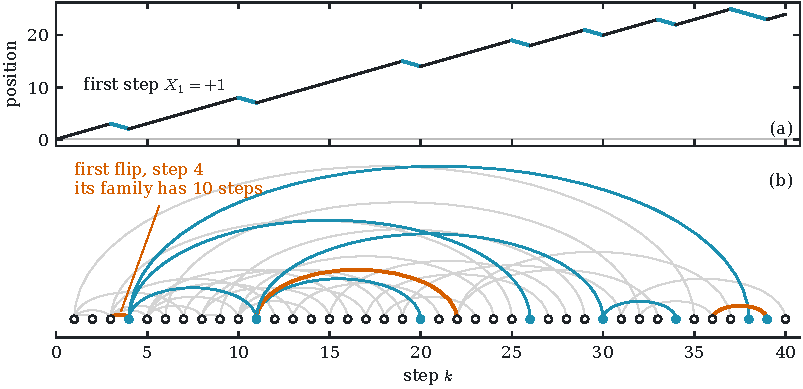
\includegraphics[width=\textwidth]{figures/family}
\caption{One elephant walk with $N=40$ steps and $\varepsilon=0.07$. (a) The position against
the step. The steps that disagree with the first step are drawn heavier and in blue. (b) The memory tree of
the same walk. Step $k+1$ copies the step at the left end of its arc, and the arcs drawn heavier
are flips. A step disagrees with the first step exactly when the path from it to step $1$
crosses an odd number of flips (Lemma~\ref{lem:tree}). The first flip, at step $4$, turns its
family of ten steps. The flip at step $22$, inside that family, turns its own family of three
steps back, and the flip at step $39$ turns only that step.}
\label{fig:family}
\end{figure}

For $k_0\ge1$ let $(M^{[k_0]}_k)_{k\ge k_0}$ be the Markov chain with
$M^{[k_0]}_{k_0}=0$ and the transition probabilities $r_k(b)$ of $M$. It is
the count of disagreeing steps for a walk whose first $k_0$ steps are forced
to agree. So $M^{[1]}$ has the law of $M$. We write $Y_d=M^{[1]}_d$, and
$Z^{(j)}_t=M^{[j-1]}_t$ for $j\ge2$ and $t\ge j-1$. In a random recursive tree
on $[N]=\{1,\dots,N\}$, vertex $k+1$ is joined to a uniform vertex of $[k]$,
independently for $k=1,\dots,N-1$. We write $\mathcal T_v$ for the subtree of
$v$, that is, $v$ and its descendants, and we call it the family of $v$.

\begin{lemma}[tree and marks]\label{lem:tree}
Let $\mathcal T$ be the tree on $[N]$ in which the parent of $k+1$ is $U_k$.
For $2\le v\le N$ let $\mu_v=1$ if step $v$ flips the step it copies, and
$\mu_v=0$ otherwise. Then $\mathcal T$ is a random recursive tree, the marks
$\mu_v$ are i.i.d.\ Bernoulli$(\varepsilon)$ and independent of $\mathcal T$,
and $X_v=X_1(-1)^{\sigma(v)}$, where $\sigma(v)$ is the number of marks on the
path from $v$ to the root, the root excluded. So $M_N=\#\{v:\sigma(v)\text{
odd}\}$. If the marks on $2,\dots,k_0$ are set to $0$, then the number of odd
vertices in $[k]$, $k\ge k_0$, is a copy of the chain $M^{[k_0]}$.
\end{lemma}

\begin{proof}
The parent $U_k$ of $k+1$ is uniform on $[k]$ and independent of the earlier
choices, and the marks are the flip indicators. The path from $k+1$ to the
root is $k+1$ followed by the path from $U_k$, so
$\sigma(k+1)=\mu_{k+1}+\sigma(U_k)$ and, by induction on $k$,
$X_{k+1}=X_{U_k}(-1)^{\mu_{k+1}}=X_1(-1)^{\sigma(k+1)}$. Now set
$\mu_2=\dots=\mu_{k_0}=0$. If $b$ of the vertices in $[k]$ are odd, $k\ge k_0$,
then $k+1$ is odd with conditional probability $(1-\varepsilon)\frac
bk+\varepsilon(1-\frac bk)=r_k(b)$, whatever else is known about $[k]$.
\end{proof}

So a single flip at $v$ turns every step of its family
(Figure~\ref{fig:family}). For $\varepsilon\le\frac12$ K\"ursten's
coupling~\cite{kursten2016} uses bond percolation with retention probability
$1-2\varepsilon$ instead, which gives the same law of the walk. For $k\ge v$, if $\mathcal T_v$ contains $s$ of the
vertices in $[k]$, then $k+1$ joins $\mathcal T_v$ with probability $s/k$.
This is the urn of Lemma~\ref{lem:urn}, so $\lvert\mathcal T_v\rvert$ has the
law $\beta_v$ and mean $N/v$, and on average there are $N/(d(d+1))$ families
of size $d$. If $v$ is the only marked vertex, the odd vertices are those of
$\mathcal T_v$. Two or more marks have probability $O(\varepsilon^2)$ at fixed
$N$, and no mark gives $M_N=0$. So at fixed $N$ the part of $f_N(m)$ of first
order in $\varepsilon$ is exactly $\varepsilon\sum_v\beta_v(m)=x/(m(m+1))$, for
$1\le m\le N-1$ (at $m=h$ this is $c_1\varepsilon$ of
Proposition~\ref{prop:first-mutation}). This is the first-order formula
of~\cite[Eq.~(10)]{bhs2023} with one cell at the start. It is also proved in Lean
for the chain $M$ (Section~\ref{sec:verify}).

To go beyond first order we cut the tree at the first flip.

\begin{lemma}[splitting]\label{lem:split}
Let $\mathcal T$ be a random recursive tree on $[N]$, let $2\le v\le N$ and
let $S\subseteq[N]$ with $\min S=v$. Given that $\mathcal T_v$ has vertex set
$S$, the restrictions of $\mathcal T$ to $S$ and to $[N]\setminus S$,
relabeled in increasing order, are independent random recursive trees. They
are independent of the parent of $v$, which is uniform on $[v-1]$.
\end{lemma}

\begin{proof}
The tree $\mathcal T$ is uniform over the $(N-1)!$ increasing trees on $[N]$.
Its family $\mathcal T_v$ has vertex set $S$ exactly when every $u\in
S\setminus\{v\}$ has its parent in $S$ and every $u\notin S$ with $u\ge2$ has
its parent outside $S$. So, given this event, each element of $S$ other than
$v$ picks its parent freely among the smaller elements of $S$, $v$ picks any
element of $[v-1]$, and each element of $[N]\setminus S$ other than $1$ picks
freely among the smaller elements of $[N]\setminus S$. This is the claim.
\end{proof}

\begin{lemma}[the first flip]\label{lem:firstmark}
Let $V=\min\{v\ge2:\mu_v=1\}$, with $V=\infty$ and $\lvert\mathcal T_V\rvert=0$ if there is no mark. Then
$\Prob(V=j,\,\lvert\mathcal T_V\rvert=d)=\varepsilon(1-\varepsilon)^{j-2}\beta_j(d)$, and for $m\ge1$
\[
 f_N(m)=\sum_{j=2}^N\varepsilon(1-\varepsilon)^{j-2}\sum_{d=1}^{N-j+1}
 \beta_j(d)\,\Prob\bigl(d-Y_d+Z^{(j)}_{N-d}=m\bigr),
\]
where $Y_d$ and $Z^{(j)}_{N-d}$ are independent.
\end{lemma}

\begin{proof}
Marks and tree are independent, which gives the law of $(V,\lvert\mathcal T_V\rvert)$. Condition on
$V=j$ and on the vertex set $S$ of $\mathcal T_j$, with $\lvert S\rvert=d$.
The marks on $j+1,\dots,N$ are still i.i.d., and by Lemma~\ref{lem:split} the
trees on $S$ and on $[N]\setminus S$ are independent random recursive trees.
The vertices $1,\dots,j-1$ carry no mark, so $j$ is odd, and $u\in S$ is odd
exactly when the path from $u$ up to $j$, with $j$ excluded, has an even
number of marks. So by Lemma~\ref{lem:tree} for the tree on $S$ rooted at
$j$, the number of odd vertices in $S$ has the law of $d-Y_d$. Paths from
outside $S$ stay outside $S$, and the tree on $[N]\setminus S$ has the
unmarked vertices $1,\dots,j-1$ first. So by Lemma~\ref{lem:tree} its odd
count has the law of $Z^{(j)}_{N-d}$. The two counts are independent, and their
law depends on $S$ only through $d$. Sum over $j$ and $d$, and note that
$M_N=0$ if there is no mark.
\end{proof}

In words, the first flip turns its whole family except the steps of that
family that flip back, and the rest of the tree is a walk whose first $j-1$
steps agree with $X_1$. Only the law of each pair $(Y_d,Z^{(j)}_{N-d})$
enters the lemma. So from now on $(Y_d)_{d\ge1}$ is a copy of the chain
$M^{[1]}$, and $(Z^{(j)}_t)_{t\ge j-1}$ is a copy of $M^{[j-1]}$, independent
of $Y$ and of $(V,\lvert\mathcal T_V\rvert)$.

\begin{lemma}[unimodality given the first step~{\cite[Section~2, proof of Theorem~1.1]{glrs2025}}]\label{lem:unimodal}
The function $f_N$ is unimodal.
\end{lemma}

This is shown at the start of the proof of Theorem~1.1 of Gu\'erin, Laulin,
Raschel and Simon~\cite{glrs2025} (by induction on the recursion for
$Q(n,k)$ at the start of Section~2 there), for every $N$ and every memory parameter
$p=1-\varepsilon\in[0,1]$. They take the first step to be $+1$ and show that
the position after $N$ steps has a unimodal law. Given $X_1=+1$ the position
is $N-2M_N$, so this is the claim. The lemma is also proved in Lean
(Section~\ref{sec:verify}). So
$f_N$ is nondecreasing on $\{0,\dots,m_h\}$ and nonincreasing on
$\{m_h,\dots,N\}$. With a fair first step, $P_N$ mixes $f_N$ and its mirror
image. When the mode of $f_N$ is far from the center, the mixture can have
two humps, one near each end.

\subsection{The end and its neighbor}\label{sec:shape-end}

We first say heuristically why the end should fall below its neighbor once
$x>2$ (Figure~\ref{fig:shape}(a), inset). Given
$X_1=+1$, the end needs no flip at all. Its neighbor, bin $N-1$, needs one flip
that is never copied. A flip at step $j$ is never copied with probability
about $j/N$. Summing $\varepsilon j/N$ over $j$ gives a factor of about $x/2$
in favor of the neighbor.

\begin{figure}[t]
\centering
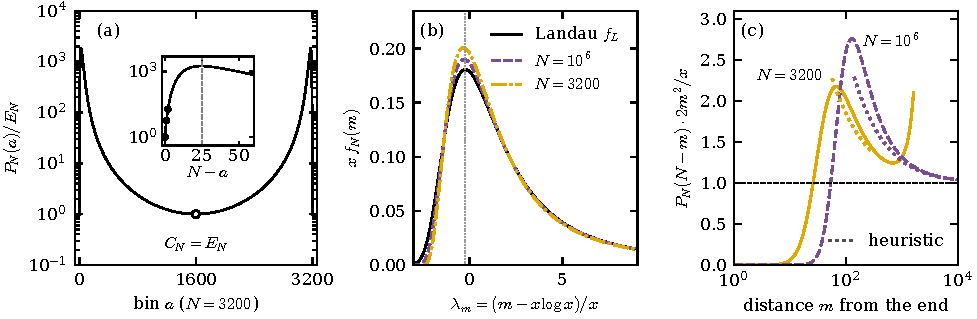
\includegraphics[width=\textwidth]{figures/shape}
\caption{The elephant walk at its crossing. (a) The law $P_N$ for $N=3200$
at its crossing $x=11.5468$, divided by the end $E_N$. The center equals the end,
and the law rises from each end to a mode and falls to the center. The inset
shows the last 60 bins, with dots at bins $N$, $N-1$ and $N-2$. The end is
below its neighbor, and the modes are 25 bins from each end (dashed). (b) The
law of $M_N$, scaled as $xf_N(m)$, against $\lambda_m=(m-x\log x)/x$, with the
Landau density $f_L$. The dotted line is its mode $\lambda_{\mathrm L}$. (c) The tail
$P_N(N-m)$ divided by $x/(2m^2)$. The dashed line is the limit 1 of
Theorem~S2.1 of Online Resource~1, and the dotted curves are the heuristic correction
$1+x(2\log m+2\gamma-3)/m$ for $2x\log x\le m\le N/x$. The rise of the
$N=3200$ curve near $m=N/2$ is the mirror term $f_N(N-m)$. At $N=10^6$ we use
$x=g_N=22.4407$.}
\label{fig:shape}
\end{figure}

\begin{theorem}[endpoint dip]\label{thm:dip}
Let $N\ge3$ and $0<\varepsilon\le\frac12$, and put $\rho_1=P_N(N-1)/E_N$.
Then
\[
 \frac{x}{2(1-\varepsilon)}<\rho_1\le\frac{x(1+1/N)^2}{2-3\varepsilon}+\frac{\varepsilon}{1-\varepsilon}.
\]
Hence the end is strictly below its neighbor if $x\ge2(1-\varepsilon)$, and
strictly above it if the right side is below $1$.
\end{theorem}

In words, when $\varepsilon$ is small the neighbor of the end is about $x/2$
times as likely as the end.

\begin{proof}
By Lemma~\ref{lem:erw-reduction}, $\rho_1=\bigl(f_N(1)+f_N(N-1)\bigr)/f_N(0)$
with $f_N(0)=(1-\varepsilon)^{N-1}$. We bound the two terms in turn.

\emph{The term $f_N(1)$.} On the event $M_N=1$ the chain moves up exactly
once, say from time $j-1$ to time $j$ with $2\le j\le N$. Before that it
stays at $0$ for $j-2$ steps, each with probability
$1-r_t(0)=1-\varepsilon$. The move up has probability $\varepsilon$. After it
the chain stays at $1$ at the times $k=j,\dots,N-1$, each with probability
$1-r_k(1)=(1-\varepsilon)(1-c'/k)$, where
$c'=(1-2\varepsilon)/(1-\varepsilon)\in[0,1]$. Multiplying and summing over
$j$ gives
\[
 f_N(1)=\varepsilon(1-\varepsilon)^{N-2}\sum_{j=2}^N\vartheta_j,\qquad
 \vartheta_j=\prod_{k=j}^{N-1}\Bigl(1-\frac{c'}k\Bigr).
\]
For the lower bound we use $c'\le1$. Then
$\vartheta_j\ge\prod_{k=j}^{N-1}(1-1/k)=(j-1)/(N-1)$, and these lower bounds sum to
$N/2$ over $2\le j\le N$. So $f_N(1)/f_N(0)\ge x/(2(1-\varepsilon))$. For
the upper bound, $1-c'/k\le e^{-c'/k}$ and $\sum_{k=j}^{N-1}1/k\ge\log(N/j)$
give $\vartheta_j\le(j/N)^{c'}$. As $(t/N)^{c'}$ is nondecreasing in $t$, we can compare
the sum with an integral, namely
\[
 \sum_{j=2}^N\vartheta_j\le\int_2^{N+1}\Bigl(\frac tN\Bigr)^{c'} dt
 \le\frac{N(1+1/N)^{c'+1}}{c'+1}\le\frac{N(1+1/N)^2(1-\varepsilon)}{2-3\varepsilon},
\]
using $c'\le1$ and $1/(c'+1)=(1-\varepsilon)/(2-3\varepsilon)$. So
$f_N(1)/f_N(0)\le x(1+1/N)^2/(2-3\varepsilon)$.

\emph{The term $f_N(N-1)$.} The event $M_N=N-1$ needs an up move at every
time. The first has probability $r_1(0)=\varepsilon$, and the one at time
$k\ge2$ has probability
$r_k(k-1)=1-\varepsilon-(1-2\varepsilon)/k\in[\frac12,1-\varepsilon]$. So
$0<f_N(N-1)\le\varepsilon(1-\varepsilon)^{N-2}$. This makes the lower bound
strict and gives the term $\varepsilon/(1-\varepsilon)$ in the upper bound.
\end{proof}

\begin{corollary}[the dip at the crossing]\label{cor:dip}
Let $N\ge4$ be even and suppose that $x_N\ge2(1-\varepsilon_N)$. Then at the
crossing $E_N=C_N<P_N(N-1)$, and $P_N$ is not unimodal.
\end{corollary}

\begin{proof}
By Proposition~\ref{prop:mlr}, $\varepsilon_N<\frac12$, so
Theorem~\ref{thm:dip} gives $P_N(N-1)>E_N=C_N$. Suppose that $P_N$ is
nondecreasing on $\{0,\dots,a_0\}$ and nonincreasing on $\{a_0,\dots,N\}$.
It is symmetric about $h$, so we may replace $a_0$ by $N-a_0$ and assume
$a_0\le h$. Then $P_N(a)\le C_N$ for every $a\ge h$, including $a=N-1$, which
is a contradiction.
\end{proof}

The hypothesis $x_N\ge2(1-\varepsilon_N)$ says that
$\varepsilon_N\ge2/(N+2)$. By Proposition~\ref{prop:mlr} it holds exactly
when $C_N\le E_N$ at $\varepsilon=2/(N+2)$. We now show that this is so for
every even $N\ge8$. For $N\ge1688$ we use Theorem~\ref{thm:erw-bounds}(b),
whose constant $5200$ uses an enclosure in ball arithmetic.
For smaller $N$ its hypothesis fails at $\varepsilon=2/N$. There we use a certified
enclosure of $\varepsilon_N$, computed as in the proof of
Proposition~\ref{prop:convex-certified}, and for $N=8$ an exact computation.

\begin{proposition}[the hypothesis holds from $N=8$ on, computer-assisted]\label{prop:dip-hyp}
For every even $N\ge8$ we have $C_N<E_N$ at $\varepsilon=2/(N+2)$, and hence
$x_N>2(1-\varepsilon_N)$. So for every even $N\ge8$, at the crossing
$E_N=C_N<P_N(N-1)$, and $P_N$ is not unimodal. For $N=2$, $4$ and $6$ the
hypothesis of Corollary~\ref{cor:dip} fails.
\end{proposition}

In words, for every even $N$ from $8$ on the end is below its neighbor at the crossing, so
the law has a hump on each side of the center.

\begin{proof}
\emph{The range $N\ge1688$.} Take $\varepsilon=2/N$. Then
$\varepsilon(1+\log N)\le\frac1{100}$, so Theorem~\ref{thm:erw-bounds}(b)
gives $C_N\le\frac8{N(N+2)}N^{4/N}e^{10400/N}$. The right side decreases in
$N$ and is below $1.4\cdot10^{-3}$ at $N=1688$. Since $\log(1-y)\ge-y-y^2$
for $0\le y\le\frac12$, we also have
$E_N=\frac12(1-\frac2N)^{N-1}\ge\frac12e^{-2-2/N}>0.06$. So $C_N<E_N$ at
$\varepsilon=2/N$, and Proposition~\ref{prop:mlr} gives $\varepsilon_N>2/N$.
Hence $C_N<E_N$ at $\varepsilon=2/(N+2)$ as well.

\emph{The range $8\le N<1688$.} For $N=8$ the ratio $C_N/E_N$ at
$\varepsilon=2/(N+2)$ is exactly $\frac{67903}{71680}<1$. For even
$10\le N\le2000$ the script \texttt{certify\_center.py} encloses
$\varepsilon_N$ in ball arithmetic as in the proof of
Proposition~\ref{prop:convex-certified}, and it checks by an exact rational
comparison that the lower end of the enclosure lies above $2/(N+2)$. So
$\varepsilon_N>2/(N+2)$, and Proposition~\ref{prop:mlr} gives $C_N<E_N$ at
$\varepsilon=2/(N+2)$. The ratio of the lower end to $2/(N+2)$ is at least
$1.107$, with its minimum at $N=10$.

\emph{The three smallest $N$.} At $\varepsilon=2/(N+2)$ the ratio $C_N/E_N$ is
exactly $2$, $\frac53$ and $\frac{508}{405}$ for $N=2$, $4$ and $6$, so
$\varepsilon_N<2/(N+2)$ there. These ratios and the one for $N=8$ are computed
in exact rational arithmetic by \texttt{certify\_elephant.py}. The last claim of the proposition about
$N\ge8$ is Corollary~\ref{cor:dip}.
\end{proof}

By Lemma~\ref{lem:unimodal}, $P_N$ is always a mixture
of two unimodal laws (namely $f_N$ and its mirror image), as is the limit
law in~\cite[eq.~(1)]{glrs2025}.

\subsection{The bulk}

The steps that disagree with $X_1$ lie in the flipped families. Recall the
compound Poisson law $\CP_N$ of Section~\ref{sec:results}. On average $x/(d(d+1))$ flipped vertices have a family of
size $d$. If no flipped step has a flipped descendant, which is likely when
$x^2\log N/N$ is small, then $M_N$ is the total size of the flipped families,
and this is close to the compound Poisson sum.

The law $\CP_N$ is known. Without the truncation at $d=N-1$ its
generating function is $(1-s)^{x(1-s)/s}$, which is the Lea--Coulson form of
the Luria--Delbr\"uck distribution with parameter
$x$~\cite[Eq.~(14)]{kesslerlevine2015}. Its limit after centering at $x\log x$
and dividing by $x$ is known as well~\cite[Eq.~(19)]{kesslerlevine2015}.
M\"ohle~\cite[Theorem~4.1 and Corollary~4.1]{mohle2005} proves this limit, with
the characteristic function $e^{B(t)}$ of Section~\ref{sec:results} and the
real integral for its
density that we use in Lemma~\ref{lem:landau-mode}. His Corollary~4.2 is a
local limit theorem for the untruncated law, uniform on the lattice, as the
parameter tends to infinity through the integers, and it has no rate. The
same stable law appears for the root cluster of a random recursive
tree~\cite{bertoin2014ejp}, and~\cite[Eqs.~(58)--(60)]{bhs2023} use it for
the reversible chain itself, without error bounds. So the limit law in the
two theorems below is not new. What they add is the truncation at $d=N-1$, a
rate (an explicit error in Theorem~\ref{thm:cp} and an absolute constant in
Theorem~\ref{thm:landau}), and the transfer to the elephant walk in sup norm. Numerical values of $f_L$ and
of its mode are standard (see K\"olbig and Schorr~\cite{ks1984}). What
Lemma~\ref{lem:landau-mode} adds is a certified enclosure.

\begin{theorem}[compound Poisson bulk]\label{thm:cp}
For $N\ge2$ and $0<\varepsilon\le\frac14$,
\[
 \sup_{m\ge0}\bigl\lvert f_N(m)-\CP_N(m)\bigr\rvert\le\delta_B
 :=\frac{x^2\log N}{N}+\frac{4x^2}{N}e^{4x^2/N}+\frac{4x^2(H_N^2+H_N)}{N}.
\]
\end{theorem}

In words, bin by bin the law of the number of disagreeing steps is within
$\delta_B$ of the compound Poisson law, and $\delta_B=O(x^2\log^2N/N)$ when
$x^2\le N$.

\paragraph{Idea of the proof.}
The proof is in Appendix~\ref{app:bulk}. Let $Z_+$ be the total size of the
flipped families. Then $M_N=Z_+$ unless some flipped step has a flipped
descendant, and this has probability at most $x^2\log N/N$. Given the tree,
$Z_+$ is a sum of independent terms, so its characteristic function is a
product, and the product is close to $e^{\varepsilon F}$ with
$F=\sum_v(e^{i\theta\lvert\mathcal T_v\rvert}-1)$. The mean of
$\varepsilon F$ is exactly the logarithm of the characteristic function of
$\CP_N$. So it remains to show that $F$ is close to its mean. For this we
use the Efron--Stein inequality~\cite{efronstein1981}. Changing the parent
of one vertex changes the family sizes only along two paths to the root, and
these paths have length of order $\log N$.

The families of size up to about $x$ add up to nearly $x\log x$, and the few
families of size of order $x$ give fluctuations of order $x$. So we center
$M_N$ at $x\log x$ and divide by $x$, which gives the coordinate $\lambda_m$
and the Landau density $f_L$ of Section~\ref{sec:results}. It is a stable
density with index one. We show in
Appendix~\ref{app:bulk} that $e^B$ is the characteristic function of a
probability law of class $L$, so that $f_L$ is a unimodal probability
density by~\cite{yamazato1978}.

\begin{theorem}[Landau limit]\label{thm:landau}
Assume~\eqref{eq:H}. There is an absolute constant $C$ such that the
following hold.
\begin{enumerate}[(a)]
\item For every integer $m\ge0$, $\bigl\lvert x\,\CP_N(m)-f_L(\lambda_m)\bigr\rvert
\le C\bigl(\frac{1+\log x}x+\frac xN\bigr)$.
\item For every integer $m\ge0$, $\bigl\lvert xf_N(m)-f_L(\lambda_m)\bigr\rvert
\le C\bigl(\frac{1+\log x}x+\frac xN\bigr)+x\delta_B$.
\item If $x\to\infty$ and $x^3\log^2N/N\to0$, then $(M_N-x\log x)/x$
converges in law to the law with density $f_L$.
\end{enumerate}
We do not compute $C$.
\end{theorem}

In words, near the crossing the number of disagreeing steps is about
$x\log x$, with fluctuations of order $x$ that follow the Landau law, bin by
bin (Figure~\ref{fig:shape}(b)). Both conditions of (c) hold at the crossing, by
Theorem~\ref{thm:erw-crossing}.

\paragraph{Idea of the proof.}
The proof is in Appendix~\ref{app:bulk}. If we allow every jump size
$d\ge1$, the characteristic function of the compound Poisson law is
$e^{x\chi(e^{i\theta})}$ with $\chi(s)=(1-s)\log(1-s)/s$, and the jumps
$d\ge N$ change it little. For small $\theta$ we have
$\chi(e^{i\theta})=-i\theta\log(-i\theta)+O(\theta^2\lvert\log\lvert\theta\rvert\rvert)$.
With $\theta=t/x$ the exponent becomes $B(t)+it\log x$ plus an error of
order $t^2\log x/x$. The term $it\log x$ is the centering at $x\log x$. Both
characteristic functions decay like $e^{-c\lvert t\rvert}$, so Fourier
inversion turns this into a bound for each bin. Part (b) then follows from
Theorem~\ref{thm:cp}.

To locate the modes we need to know that $f_L$ is curved at its maximum.

\begin{lemma}[the mode of the Landau density, computer-assisted]\label{lem:landau-mode}
\begin{enumerate}[(a)]
\item The density $f_L$ has exactly one mode $\lambda_{\mathrm L}$, and
$-0.22278299<\lambda_{\mathrm L}<-0.22278297$.
\item The derivative vanishes at the mode, $f_L'(\lambda_{\mathrm L})=0$, and
$-0.0792\le f_L''(\lambda)\le-0.0786$ for
$-0.2229\le\lambda\le-0.2227$.
\item For every real $\lambda$,
$f_L(\lambda_{\mathrm L})-f_L(\lambda)\ge\kappa_L\min\{1,(\lambda-\lambda_{\mathrm L})^2\}$ with
$\kappa_L=2.6\cdot10^{-10}$.
\end{enumerate}
\end{lemma}

The proof is in Appendix~\ref{app:bulk}. It is computer-assisted. We turn the
Fourier integral into the real integral
$f_L(\lambda)=\frac1\pi\int_0^\infty e^{-s\log s-\lambda s}\sin(\pi s)\,ds$.
Then we enclose $f_L'$ at four points (namely $-0.2229$, $-0.2227$,
$-0.22278299$ and $-0.22278297$) and $f_L''$ on the interval
$[-0.2229,-0.2227]$. We use ball arithmetic at 128 bits (python-flint 0.9.0,
which wraps Arb) and the rigorous integration algorithm
of~\cite{johansson2018} on $[2^{-20},30]$, with explicit bounds for the rest
(\texttt{certify\_elephant.py}). The run takes under a second. Part (c) follows from (b) and the
unimodality of $f_L$.

\begin{corollary}[where the modes are]\label{cor:mode-location}
\begin{enumerate}[(a)]
\item Assume~\eqref{eq:H}. Let $\kappa_L$ be as in
Lemma~\ref{lem:landau-mode}(c), let $E_1$ be the bound of
Theorem~\ref{thm:landau}(b), and put
\[
 E'=E_1+\frac{16x^2H_N}{N^2}+\frac{\lVert f_L''\rVert_\infty}{8x^2}.
\]
If $E'<\kappa_L/2$ and $m_h\le N/4$, then every mode $a^*\ge N/2$ of $P_N$
satisfies $\lvert m^*-x\log x-\lambda_{\mathrm L}x\rvert\le x\sqrt{2E'/\kappa_L}$,
and so does every mode of $f_N$.
\item Let $N\to\infty$ over even $N$. At the crossing, with $x=x_N$, every mode
$a^*\ge N/2$ of $P_N$ has
\[
 m^*=x\log x+\lambda_{\mathrm L}x+O\bigl(\sqrt{x\log x}\bigr),
\]
and so has the largest mode $m_h$ of $f_N$.
\end{enumerate}
In (a) the only constant that we do not compute is the constant $C$ of
Theorem~\ref{thm:landau}, which enters $E_1$. (Here
$\lVert f_L''\rVert_\infty\le16/\pi^4$, since $\lvert e^{B(t)}\rvert=e^{-\pi\lvert t\rvert/2}$.)
We do not compute the implied constant in (b).
\end{corollary}

In words, each hump of the law at the crossing sits about
$x\log x-0.2228\,x$ bins from its end. The proof is in
Appendix~\ref{app:bulk-cor}. It compares $f_N$ at a mode with $f_N$ at the
integer nearest to $x\log x+\lambda_{\mathrm L}x$, and uses
Theorem~\ref{thm:landau}(b) and Lemma~\ref{lem:landau-mode}(c).

\begin{remark}[how good the bulk approximation is]\label{rem:bulk}
The bounds of this subsection are far from sharp at the sizes we can
compute. At $N=10^6$ and $x=22.4407$ the bound $\delta_B$ is still about
$0.46$, but there the computed law has
$\lvert f_N(m)/\CP_N(m)-1\rvert\le3.6\cdot10^{-4}$ for $1\le m\le10^4$. At
every tested crossing $m^*$ equals the mode of $\CP_N$. We do not compute the
error term in Corollary~\ref{cor:mode-location}(b). Its proof needs the
bound of Theorem~\ref{thm:landau}(b) to be below $\kappa_L/2$, where
$\kappa_L$ is the constant of Lemma~\ref{lem:landau-mode}(c), and
numerically the best $\kappa_L$ is about $0.026$. These numbers are computed
in double precision and are not used in any proof.
\end{remark}

\subsection{The tail}

Beyond the humps the law falls like $x/(2m^2)$. Theorem~S2.1 of Online
Resource~1 proves that
$P_N(N-m)=\frac{x}{2m^2}(1+o(1))$ for even $N$ with $x\ge1$ and
$x\log^2N/N\to0$, uniformly for $\omega_Nx\log^2(x+1)\le m\le\delta'_NN$, for
every $\omega_N\to\infty$ with $\omega_Nx\log^2(x+1)=o(N)$ and every
$\delta'_N\to0$.

At $N=10^6$, $x=22.4407$ and $m=10^4$ the computed ratio
$P_N(N-m)/(x/(2m^2))$ is $1.03777$. Heuristically, at moderate $m$ the law
$\CP_N$ suggests $f_N(m)\,m(m+1)/x\approx1+x(2\log m+2\gamma-3)/m$, which we
do not prove. This factor is still about $2$ near $m=70$ when $N=3200$
(Figure~\ref{fig:shape}(c)).

\subsection{Convexity between the humps}\label{sec:convex}

\begin{definition}[convex between the humps]\label{def:convex}
Let $N\ge10$. The law at the crossing is \emph{convex between the humps} if,
for $x=x_N$ and every mode $a^*\ge N/2$ of $P_N$ with $m^*=N-a^*$, the second
difference $P_N(a-1)-2P_N(a)+P_N(a+1)$ is positive for
$2m^*+1\le a\le N-2m^*-1$.
\end{definition}

With the symmetry of the law, this makes $P_N$ strictly convex on
$[2m^*,N-2m^*]$, so $h$ is its unique minimizer there (the two central bins
for odd $N$). At the crossing $m^*=o(N)$ by
Corollary~\ref{cor:mode-location}(b), so for large even $N$ the property
makes the center the unique interior minimum (Corollary~\ref{cor:unique-min}).
This subsection proves the property for all large $N$, even
(Theorem~\ref{thm:convex-large}) or odd (Proposition~\ref{prop:odd}), and,
with a certified computation, for $10\le N\le2000$
(Proposition~\ref{prop:convex-certified}). For every even $N\ge8$ and every
odd $N\ge1689$ it reduces the property to one inequality
(Corollary~\ref{cor:one-point} and Proposition~\ref{prop:odd}(c)). The
constants of the large-$N$ results are not computed, so the following is
open.

\begin{conjecture}[convexity between the humps]\label{conj:convex}
For every $N>2000$ the law at the crossing is convex between the humps.
\end{conjecture}

In double precision the law at the crossing is also convex between the humps
for $N=3200$, $6400$, $12800$ and $25600$. The definition leaves out the two
endpoints $a=2m^*$ and
$a=N-2m^*$, because there the second difference is not positive for some
$N\le51$. Heuristically, between the humps $P_N(a)$ is close to
$\frac x2\bigl[\frac1{a(a+1)}+\frac1{(N-a)(N-a+1)}\bigr]$, which is strictly
convex in $a$. We also leave open
the tail between $x\log x$ and $x\log^2x$ (Remark~\ref{rem:convex-open} discusses $N_1$ and $N_1'$).

Throughout this subsection $0<\varepsilon<\frac12$ and $c=1-2\varepsilon$, so
that $r_t(b)=\varepsilon+cb/t$. For $t\ge1$ and every integer $a$ we write
$P_t(a)=\Prob(A_t=a)$, which is $0$ unless $0\le a\le t$, and
\[
 D_t(a)=P_t(a+1)-2P_t(a)+P_t(a-1).
\]
We also put $s_t=D_t(1)=P_t(0)-2P_t(1)+P_t(2)$ for $t\ge2$.

\begin{lemma}[recurrence for the second difference]\label{lem:D-rec}
For every $t\ge1$ and every integer $a$,
\begin{align}
 P_{t+1}(a)&=\bigl(1-r_t(a)\bigr)P_t(a)+r_t(a-1)\,P_t(a-1),\label{eq:P-rec}\\
 D_{t+1}(a)&=\bigl(1-r_t(a+1)\bigr)D_t(a)+r_t(a-2)\,D_t(a-1).\label{eq:D-rec}
\end{align}
Also $P_t(a)=P_t(t-a)$ and $D_t(a)=D_t(t-a)$. The same two recurrences hold
with $f_t(m)$ in place of $P_t(a)$.
\end{lemma}

\begin{proof}
Given $A_t=a$, the copied step is $+1$ with probability $a/t$, so step $t+1$
is $+1$ with probability $(1-\varepsilon)\frac at+\varepsilon(1-\frac
at)=r_t(a)$. This gives \eqref{eq:P-rec} for $0\le a\le t+1$, where at $a=0$ and at
$a=t+1$ the formula has one extra term, namely $r_t(-1)P_t(-1)$ or
$(1-r_t(t+1))P_t(t+1)$, and this term is $0$ because $P_t(-1)=P_t(t+1)=0$. For
other $a$ every term vanishes. The
symmetry of $P_t$ is Lemma~\ref{lem:erw-reduction}, and it gives the symmetry
of $D_t$. The chain $M$ of Lemma~\ref{lem:erw-reduction} has the same
transition probabilities, so \eqref{eq:P-rec} holds for $f_t$ as well.

For \eqref{eq:D-rec} put $\varsigma=c/t$, so that $r_t(b+1)=r_t(b)+\varsigma$.
We insert \eqref{eq:P-rec} at $a+1$, $a$ and $a-1$ into the definition of
$D_{t+1}(a)$ and collect the coefficients of $P_t(a+1)$, $P_t(a)$, $P_t(a-1)$
and $P_t(a-2)$. They are
\[
 1-r_t(a+1),\qquad 3r_t(a)-2,\qquad 1-3r_t(a-1),\qquad r_t(a-2).
\]
The right side of \eqref{eq:D-rec} has the coefficients $1-r_t(a+1)$,
$-2+2r_t(a+1)+r_t(a-2)$, $1-r_t(a+1)-2r_t(a-2)$ and $r_t(a-2)$. The second
ones agree because $2r_t(a+1)+r_t(a-2)=3r_t(a)$, and the third ones agree
because $r_t(a+1)+2r_t(a-2)=3r_t(a-1)$.
\end{proof}

Trinas and Valle~\cite[(2.2)]{tv2026} write \eqref{eq:P-rec} for the mass
function of the position, which is the forward equation of the counting
chain of Lemma~\ref{lem:erw-reduction}, and they use it for a local limit
theorem in the superdiffusive regime. In~\cite[(4.10)]{tv2026} they write
the analogue of~\eqref{eq:D-rec} for differences of higher order, and they
use it at a fixed memory parameter in a certified study of log-concavity. We use
\eqref{eq:D-rec} for signs.
The coefficients in \eqref{eq:D-rec} are positive when $2\le a\le t-1$. So the
second difference moves like a mass that is partly killed, and its sign can
change only through what enters at the two edges. The next lemma is the
elementary form of the variation diminishing property that we need.

For a finite list $z$ of real numbers let $\operatorname{sp}(z)$ be its sign
pattern. We delete the zeros of $z$, replace each entry by its sign, and merge
equal neighbors. So $\operatorname{sp}(z)$ is a list of alternating signs. For
two such lists we write $p\preceq q$ if $p$ is a subsequence of $q$. We put
$\Pi_5=(+,-,+,-,+)$ and $\Pi_3=(+,-,+)$.

\begin{lemma}[one step]\label{lem:interleave}
Let $\zeta=(\zeta_1,\dots,\zeta_n)$ be real, and let
$\eta_i=A_i\zeta_i+B_i\zeta_{i+1}$ for $1\le i\le n-1$ with $A_i\ge0$ and
$B_i\ge0$. Let $w=(\zeta_1,\eta_1,\zeta_2,\eta_2,\dots,\eta_{n-1},\zeta_n)$.
Then $\operatorname{sp}(w)=\operatorname{sp}(\zeta)$ and
$\operatorname{sp}(\eta)\preceq\operatorname{sp}(\zeta)$.
\end{lemma}

We prove this in Appendix~\ref{app:signs-step}.

\begin{lemma}[the sequence next to the end]\label{lem:level-one}
For every $t_1\ge2$ we have $\operatorname{sp}(s_2,s_3,\dots,s_{t_1})\preceq\Pi_3$.
Also, for every $0\le\varepsilon\le1$, the numbers $s_3$ and $s_4$ do not both vanish.
\end{lemma}

We prove this in Appendix~\ref{app:signs-level}.

\begin{theorem}[at most five blocks]\label{thm:five-blocks}
Let $N\ge3$ and $0<\varepsilon<\frac12$. Then
\[
 \operatorname{sp}\bigl(D_N(1),D_N(2),\dots,D_N(N-1)\bigr)\preceq(+,-,+,-,+).
\]
So the second difference of $P_N$ changes sign at most four times on
$\{1,\dots,N-1\}$. The same holds for the second difference of $f_N$.
\end{theorem}

In words, for every $N\ge3$ and every $0<\varepsilon<\frac12$ the law has at most two
concave stretches. When it has two, the stretch between them is convex.

We prove this in Appendix~\ref{app:signs-five}.

The next theorem is the step that turns one sign into a whole convex
stretch. Its idea is short. A sign change from negative to positive at
$a_0<a_1$, together with its mirror image, gives the signs $-,+,+,-$ at
$a_0<a_1<N-a_1<N-a_0$. A negative second difference in between would add a
fifth alternating sign, which Theorem~\ref{thm:five-blocks} forbids. A zero
in between is subtler. We follow it back in time through \eqref{eq:D-rec},
whose coefficients are positive, so a zero has two zero parents unless its
parents have opposite signs, and opposite signs would again give five
alternating signs. Going back to $t=5$ forces $s_3=s_4=0$, which
Lemma~\ref{lem:level-one} rules out.

\begin{theorem}[no holes]\label{thm:no-holes}
Let $N\ge5$ and $0<\varepsilon<\frac12$. Let $1\le a_0<a_1\le N/2$ be integers
with $D_N(a_0)<0<D_N(a_1)$. Then $D_N(a)>0$ for every $a_1\le a\le N-a_1$.
\end{theorem}

In words, once the law has turned convex to the right of its left hump, it
stays strictly convex up to the mirror image of that point.

We prove this in Appendix~\ref{app:signs-holes}.

\begin{corollary}[one inequality is enough]\label{cor:one-point}
Let $N\ge8$ be even and $x=x_N$, or let $N\ge5$ and $0<\varepsilon<\frac12$
be such that $P_N(0)<P_N(1)$. Let $a^*$ be any mode of $P_N$ and
$m^*=N-a^*$. If $D_N(a_1)>0$ for some integer $a_1$ with $m^*<a_1\le2m^*+1$
and $a_1\le N/2$, then $D_N(a)>0$ for every $2m^*+1\le a\le N-2m^*-1$. In
particular $P_N$ is strictly convex on $[2m^*,N-2m^*]$ as soon as
$D_N(2m^*+1)>0$.
\end{corollary}

\begin{proof}
At the crossing with $N\ge8$ even, $P_N(0)=E_N<P_N(N-1)=P_N(1)$ by
Proposition~\ref{prop:dip-hyp}. Let $a_0$ be the smallest maximizer of $P_N$.
Then $1\le a_0\le m^*$, because $P_N(0)<P_N(1)$ and $P_N(m^*)=P_N(a^*)$ is the
maximum. Also $P_N(a_0-1)<P_N(a_0)\ge P_N(a_0+1)$, so $D_N(a_0)<0$. Now
Theorem~\ref{thm:no-holes} applies to $a_0<a_1$.
\end{proof}

The condition $a_1\le N/2$ costs nothing at $a_1=2m^*+1$, because
$2m^*+1\le N/2$ whenever the range $2m^*+1\le a\le N-2m^*-1$ is not empty.
If $a^*<N/2$, then $m^*>N/2$, and no $a_1$ meets the conditions.

\begin{theorem}[convexity between the humps for large $N$]\label{thm:convex-large}
There is $N_1$ such that the law at the crossing is convex between the humps
for every even $N\ge N_1$. That is, for even $N\ge N_1$, $x=x_N$ and every mode $a^*\ge N/2$
of $P_N$ with $m^*=N-a^*$,
\[
 P_N(a-1)-2P_N(a)+P_N(a+1)>0\qquad\text{for }2m^*+1\le a\le N-2m^*-1 .
\]
We do not compute the threshold $N_1$ (Remark~\ref{rem:convex-open}).
\end{theorem}

\paragraph{Idea of the proof.}
By Corollary~\ref{cor:one-point} it is enough to find one point of strict
convexity between $m^*$ and $2m^*+1$. If there were none, $P_N$ would be
concave on $[m^*,2m^*+2]$, and then its value halfway would be at least half of
its maximum. The Landau limit shows that the value halfway is much smaller.

\begin{proof}
Let $N$ be even and large, and let $x=x_N$ and $\varepsilon=\varepsilon_N$. By
Theorem~\ref{thm:erw-crossing}, $x\to\infty$ and $x=O(\log N)$. So \eqref{eq:H}
holds, and $(1+\log x)/x$, $x/N$ and
$x\delta_B=O(x^3\log^2N/N)$ tend to $0$. So by Theorem~\ref{thm:landau}(b)
there are numbers $\Theta_N\to0$ with
\begin{equation}\label{eq:llt-used}
 \bigl\lvert xf_N(m)-f_L(\lambda_m)\bigr\rvert\le\Theta_N\qquad\text{for every integer }m\ge0 .
\end{equation}
The density $f_L$ is continuous, because it is the Fourier transform of an
integrable function. It is unimodal with mode $\lambda_{\mathrm L}$
(Lemma~\ref{lem:landau-mode}), so it is nonincreasing on
$[\lambda_{\mathrm L},\infty)$, and it is integrable. So
$f_L(\lambda)\to0$ as $\lambda\to\infty$. We write $o(1)$ for a quantity that
is bounded in absolute value by a function of $N$ alone that tends to $0$.

\emph{Step 1: the mirror term.} Let $0\le m\le N/2$. Then
$\lambda_{N-m}\ge\frac N{2x}-\log x\to\infty$. So \eqref{eq:llt-used} gives
$xf_N(N-m)\le f_L(\lambda_{N-m})+\Theta_N=o(1)$. Since
$P_N(m)=P_N(N-m)=\frac12[f_N(m)+f_N(N-m)]$, we get
\[
 2xP_N(m)=f_L(\lambda_m)+o(1)\qquad\text{uniformly for }0\le m\le N/2 .
\]

\emph{Step 2: the mode.} Let $m_0$ be the integer part of
$x\log x+\lambda_{\mathrm L}x$. Then $0\le m_0\le N/2$ and
$\lvert\lambda_{m_0}-\lambda_{\mathrm L}\rvert\le1/x$, so Step~1 and the continuity of
$f_L$ give $2xP_N(m_0)=f_L(\lambda_{\mathrm L})+o(1)$. Now $P_N(m^*)\ge P_N(m_0)$ and
$m^*\le N/2$, so Step~1 at $m^*$ gives
$f_L(\lambda_{m^*})\ge f_L(\lambda_{\mathrm L})-o(1)$. By
Lemma~\ref{lem:landau-mode}(c) this forces
$\lvert\lambda_{m^*}-\lambda_{\mathrm L}\rvert\le1$ for large $N$. Hence
\[
 x\log x+(\lambda_{\mathrm L}-1)x\le m^*\le x\log x+(\lambda_{\mathrm L}+1)x,\qquad
 2xP_N(m^*)\ge f_L(\lambda_{\mathrm L})-o(1).
\]
In particular $m^*\to\infty$ and $2m^*+2\le N/2$ for large $N$.

\emph{Step 3: halfway.} Let $v=m^*+\lfloor m^*/2\rfloor$. Then
$v\ge\frac32m^*-1$, so by Step~2
\[
 \lambda_v\ge\tfrac12\log x+\tfrac32(\lambda_{\mathrm L}-1)-\tfrac1x\to\infty .
\]
Also $v\le N/2$. So Step~1 gives $2xP_N(v)=f_L(\lambda_v)+o(1)=o(1)$. Since
$f_L(\lambda_{\mathrm L})>0$, Step~2 shows that $P_N(v)<\frac12P_N(m^*)$ for large $N$.

\emph{Step 4: a point of convexity.} Suppose that $D_N(a)\le0$ for every
$m^*<a\le2m^*+1$. Then $P_N$ is concave on the integers of $[m^*,2m^*+2]$.
With $u=m^*$ and $w=2m^*+2$ this gives
\[
 P_N(v)\ge\frac{w-v}{w-u}P_N(u)+\frac{v-u}{w-u}P_N(w)\ge\frac{w-v}{w-u}P_N(m^*)
 \ge\tfrac12P_N(m^*),
\]
because $w-v\ge\frac12(m^*+2)=\frac12(w-u)$. This contradicts Step~3. So
$D_N(a_1)>0$ for some $m^*<a_1\le2m^*+1$, and $a_1\le N/2$ by Step~2.
Corollary~\ref{cor:one-point} gives the claim.
\end{proof}

\begin{lemma}[the center from convexity]\label{lem:center-convex}
Let $N\ge8$ be even and $x=x_N$. Let $a^*\ge N/2$ be a mode of $P_N$ and $m^*=N-a^*$.
Suppose that $2m^*+1\le N/2$ and that $D_N(a)>0$ for every $2m^*+1\le a\le N-2m^*-1$. Then
$P_N(a)>C_N$ for every $1\le a\le N-1$ with $a\ne h$.
\end{lemma}

In words, if the law is strictly convex between the humps and the stretch between the humps
contains the center, then the center is the unique lowest interior bin.

\paragraph{Idea of the proof.}
Between the humps the law is strictly convex and symmetric, so the center is its only minimum
there. Outside, a bin as low as the center would be a second valley. A valley needs a point of
convexity with points of concavity on both sides, and with the mirror image this gives more
changes of sign of the second difference than Theorem~\ref{thm:five-blocks} allows.

\begin{proof}
Write $b=2m^*$, so that $b+1\le h$, and put $\delta(a)=P_N(a+1)-P_N(a)$.

\emph{Between the humps.} Since $D_N(a)=\delta(a)-\delta(a-1)>0$ for $b+1\le a\le N-b-1$, the
differences $\delta(a)$ are strictly increasing for $b\le a\le N-b-1$. By symmetry
$\delta(h-1)=-\delta(h)$, and $\delta(h-1)<\delta(h)$ because $b\le h-1$. So
$\delta(h-1)<0<\delta(h)$. Hence $P_N$ is strictly decreasing on $\{b,\dots,h\}$ and strictly
increasing on $\{h,\dots,N-b\}$, and $P_N(a)>C_N$ for every $b\le a\le N-b$ with $a\ne h$. In
particular $P_N(b)>C_N$.

\emph{Near the ends.} By symmetry it is enough to treat $1\le a\le b-1$. Suppose that
$P_N(a)\le C_N$ for some such $a$, and let $k$ be the smallest index in $\{1,\dots,b\}$ at which
$P_N$ takes its least value on this set. By Proposition~\ref{prop:dip-hyp},
$P_N(1)>P_N(0)=E_N=C_N$, and $P_N(b)>C_N$. So $2\le k\le b-1$, and
$P_N(k-1)>P_N(k)\le P_N(k+1)$, which gives $D_N(k)>0$.
Next let $a'$ be the smallest index at which $P_N$ takes its largest value on $\{0,\dots,k\}$.
This value is at least $P_N(1)$, which exceeds both $P_N(0)$ and $P_N(k)$. So $1\le a'\le k-1$
and $P_N(a'-1)<P_N(a')\ge P_N(a'+1)$, which gives $D_N(a')<0$. In the same way let $a''$ be the
largest index at which $P_N$ takes its largest value on $\{k,\dots,h\}$. This value is at least
$P_N(b)$, which exceeds both $P_N(k)$ and $P_N(h)=C_N$. So $k+1\le a''\le h-1$ and
$P_N(a''-1)\le P_N(a'')>P_N(a''+1)$, which gives $D_N(a'')<0$. Finally $D_N(h)>0$ by hypothesis.

So $D_N$ has the signs $-,+,-,+$ at $a'<k<a''<h$. By the symmetry $D_N(a)=D_N(N-a)$ it has the
signs $-,+,-$ at $N-a''<N-k<N-a'$. Hence the sign pattern of $(D_N(1),\dots,D_N(N-1))$ has a
subsequence of seven alternating signs. This contradicts Theorem~\ref{thm:five-blocks}, which
allows at most five.
\end{proof}

\begin{corollary}[the center is the unique interior minimum]\label{cor:unique-min}
For every large even $N$, at the crossing, $P_N(a)>C_N$ for every
$1\le a\le N-1$ with $a\ne h$. We do not compute the threshold for $N$.
\end{corollary}

\begin{proof}
Let $N$ be large and even, and let $a^*\ge N/2$ be a mode of $P_N$ with $m^*=N-a^*$. By
Corollary~\ref{cor:mode-location}(b), $m^*=O(\log N\log\log N)$, so $2m^*+1\le N/2$ for large
$N$. By Theorem~\ref{thm:convex-large}, $D_N(a)>0$ for $2m^*+1\le a\le N-2m^*-1$. So
Lemma~\ref{lem:center-convex} applies.
\end{proof}

\begin{proposition}[small $N$, computer-assisted]\label{prop:convex-certified}
For every $10\le N\le N_{\rm c}=2000$, even or odd, the law at the crossing is
convex between the humps.
\end{proposition}

\begin{proof}
The script \texttt{certify\_convex.py} uses ball arithmetic with 160 bits
(the library Arb). For each $N$ it encloses $\varepsilon_N$ in an interval of
relative width at most $2\cdot10^{-8}$. It does so by evaluating the center
and the end at the two ends of the interval, and Proposition~\ref{prop:mlr}
then places the crossing between them. It then runs \eqref{eq:P-rec} with
$\varepsilon$ equal to this interval. Each step only multiplies and adds
enclosures of numbers in $[0,1]$, so the radii stay small. From the resulting enclosure of $P_N$ it lists every index that
can be a mode, and for each of them it checks that the enclosure of $D_N(a)$
is positive for every $2m^*+1\le a\le N-2m^*-1$. When this range is not
empty, so that $2m^*+1\le N/2$, it also checks that $D_N(a_0)<0$ for some
$1\le a_0\le2m^*$ and that $D_N(2m^*+1)>0$. By
Theorem~\ref{thm:no-holes} these two inequalities already imply the claim, so the test of
every $a$ is a second check.
\end{proof}

\begin{proposition}[odd $N$]\label{prop:odd}
Let $N\ge3$ be odd, and write $\widetilde C_N=P_N(\frac{N-1}2)=P_N(\frac{N+1}2)$ for the two
central bins. The ratio $\widetilde C_N/E_N$ is strictly increasing in $\varepsilon$, and it
equals $1$ at exactly one $\varepsilon_N\in(0,\frac12)$. Put $x_N=N\varepsilon_N$.
\begin{enumerate}[(a)]
\item For every $0<\varepsilon<\frac12$,
\[
 \widetilde C_N=\Bigl(1-\frac cN\Bigr)^{-1}C_{N+1},
\]
where $C_{N+1}$ is the center of the walk with $N+1$ steps and the same $\varepsilon$.
\item As $N\to\infty$ over odd $N$, $x_N+\log x_N=\Lambda_N+O(L^2/N)$. So both parts of
Theorem~\ref{thm:erw-crossing} hold for odd $N$ as well.
\item For every odd $N\ge1689$ we have $x_N>2$, and at the crossing $P_N(0)<P_N(1)$. So
Corollary~\ref{cor:one-point} applies to these $N$ with $x=x_N$.
\item There is $N_1'$ such that the law at the crossing is convex between the humps for
every odd $N\ge N_1'$. We do not compute the threshold $N_1'$.
\end{enumerate}
\end{proposition}

In words, the center of a walk with an even number of steps is reached from the two central bins
one step earlier, and from each of them with the same probability. So the two central bins of
an odd $N$ are the center of $N+1$ up to the factor $1-c/N$, and what we know about the crossing
for even $N$ carries over.

\begin{proof}
\emph{The crossing.} By Proposition~\ref{prop:mlr}, $P_N(k)/E_N$ is strictly increasing in
$\varepsilon$ for $k=\frac{N+1}2$. It tends to $0$ as $\varepsilon\to0$. At
$\varepsilon=\frac12$ the steps are independent and fair, so
$\widetilde C_N=\binom Nk2^{-N}>2^{-N}=E_N$. So the ratio equals $1$ at exactly one
$\varepsilon_N$, and $\varepsilon_N<\frac12$.

(a) Put $k=\frac{N+1}2$. Since $\varepsilon+\frac c2=\frac12$, we have
$r_N(k)=\frac12+\frac c{2N}$ and $r_N(k-1)=\frac12-\frac c{2N}$. So \eqref{eq:P-rec} with $t=N$
and $a=k$ gives
\[
 C_{N+1}=P_{N+1}(k)=\Bigl(\frac12-\frac c{2N}\Bigr)\bigl(P_N(k)+P_N(k-1)\bigr)
 =\Bigl(1-\frac cN\Bigr)\widetilde C_N .
\]

We prove (b), (c) and (d) in Section~S3 of Online Resource~1.
\end{proof}

\begin{proposition}[the center for $10\le N\le2000$, computer-assisted]\label{prop:center-small}
For every even $10\le N\le2000$, at the crossing, $P_N(a)>C_N$ for every $1\le a\le N-1$
with $a\ne h$.
\end{proposition}

So Corollary~\ref{cor:unique-min} holds for every even $N$ from $10$ to $2000$, and not only for
large $N$.

\begin{proof}
Let $10\le N\le2000$ be even. By Proposition~\ref{prop:convex-certified}, $D_N(a)>0$ for
$2m^*+1\le a\le N-2m^*-1$ and every mode. The script \texttt{certify\_center.py} encloses
$\varepsilon_N$ and the law $P_N$ in the same way as \texttt{certify\_convex.py}, lists every
index $a^*\ge N/2$ that can be a mode, and checks that $2(N-a^*)+1\le N/2$ for each of them. This
holds for every even $N$ in the range. So Lemma~\ref{lem:center-convex} applies.
\end{proof}

As a second check, for each even $N$
in the range the script also tests directly that the enclosure of $P_N(a)-P_N(h)$ is positive for
every $1\le a\le N-1$ with $a\ne h$, and this succeeds for all $996$ values of $N$. The smallest value of
$N/2-(2m^*+1)$ is $1$, at $N=12$.

\begin{remark}[what is still open]\label{rem:convex-open}
We do not compute the constant $N_1$ of Theorem~\ref{thm:convex-large},
because we do not compute the constant $C$ in Theorem~\ref{thm:landau}. Even with explicit constants, Step~3 needs $f_L(\frac32\lambda_{\mathrm L}+\frac12\log x)<\frac12f_L(\lambda_{\mathrm L})$ up
to the error $\Theta_N$, and at the sizes we can compute the ratio
$P_N(v)/P_N(m^*)$ is still about $0.8$. Numerically $f_L$ falls to half of its maximum at
$\lambda=2.432$. So even without the error $\Theta_N$, Step~3 needs
$\frac32\lambda_{\mathrm L}+\frac12\log x>2.432$, that is, $x>252.8$. Since
$x_N+\log x_N$ is close to $2\log N-\log8$ (Theorem~\ref{thm:erw-crossing}), this means that $N$
is above about $3.5\cdot10^{56}$. So the $N$ between $N_{\rm c}$ and $N_1$ or $N_1'$ are open, and no
computation can reach these constants as the proof stands. By Corollary~\ref{cor:one-point} and Proposition~\ref{prop:odd}(c) the whole range would
be closed by an effective proof of the single inequality $D_N(a_1)>0$ at one point
$m^*<a_1\le2m^*+1$. Numerically the convex stretch starts near $1.5\,m^*$. This agrees with
the Landau limit, because the inflection point of $f_L$ to the right of its mode is at
$\lambda=1.104$ numerically, and $x\log x+1.104\,x$ is below twice the mode
$x\log x+\lambda_{\mathrm L}x$ as soon as $x\ge4.8$. A proof along these lines would need the second
differences of $P_N$ near $2m^*$ with an error below their size. At a fixed Landau coordinate
$\lambda$ this size is of order $x^{-3}$. Near $2m^*$, however, $\lambda$ is close to $\log x$, and
$f_L''(\lambda)\sim6/\lambda^4$ as $\lambda\to\infty$, so there the Landau density suggests the
much smaller size $3/[x^3(\log x)^4]$. This is a heuristic, not a local limit theorem for second
differences. The main error in Theorem~\ref{thm:landau} is $C(1+\log x)/x$ for each value of
$xf_N$, with a constant $C$ that we do not compute, and this is far too large for the $N$ in
question.
\end{remark}

\section{Verification}\label{sec:verify}

{\sloppy
The Python computations use two independent methods for the main checks
(for example, forward and backward recursions for the elephant center
agree to about $10^{-14}$ at $N=12800$). Apart from short exact computations
that can be checked by hand, such as the ratios $C_N/E_N$ for $N=2$, $4$, $6$
and $8$ in Proposition~\ref{prop:dip-hyp}, the proofs use computation in three
places. First, some constants are values of
explicit sums and integrals, such as the 60-term sum in the proof of
Theorem~\ref{thm:erw-bounds}(b), which we enclosed in ball arithmetic. It lies
in $[102.586396,102.586398]$, so the series is below the bound $102.59$ used
in the proof even with the tail added. Any finite bound suffices for the
asymptotic statements. The value $5200$ matters for the thresholds $1688$ and
$1689$ in Proposition~\ref{prop:dip-hyp} and in Proposition~S3.1(b) of Online Resource~1, and for
the second-order bound there. Second,
Lemma~\ref{lem:landau-mode} rests on enclosures of $f_L'$ at four points and
of $f_L''$ on an interval, computed in ball arithmetic with
rigorous error bounds. These two computations are in
\texttt{certify\_elephant.py}. Lean repeats the second one with enclosures of its own, as
we describe below. Third, for every $10\le N\le2000$ the script
\texttt{certify\_convex.py} encloses the crossing $\varepsilon_N$ in ball
arithmetic and then encloses the whole law $P_N$ at the crossing.
Proposition~\ref{prop:convex-certified} rests on this computation (with its output in
\nolinkurl{data/certify_convex_output_2026-10-17.txt}). The script
\texttt{certify\_center.py} repeats it for every even $N$ in the range and
proves Proposition~\ref{prop:center-small}, and Proposition~\ref{prop:dip-hyp} for
$10\le N<1688$ (with its
output in \nolinkurl{data/certify_center_output_2026-10-17.txt}). For $5\le N\le9$,
Propositions~\ref{prop:convex-certified} and~\ref{prop:center-small} rest instead on the
checks in Lean described below. With the option
\texttt{-{}-witness} the two scripts also write a record for each $N$, with the
rational ends of the enclosure of $\varepsilon_N$, the indices that can be a
mode and the certified margins, under a header with the SHA-256 hashes of the
scripts and the versions of Python and python-flint. The records of these runs
are in \nolinkurl{data/witnesses_convex_2026-10-17.jsonl} and
\nolinkurl{data/witnesses_center_2026-10-17.jsonl}. Each of the three
\texttt{certify} scripts exits with nonzero status if any required
certification fails, and the two scripts that take a range of $N$ also refuse
an empty range.
Earlier outputs remain in \nolinkurl{data}, with their old statement
numbers listed in \nolinkurl{paperD/README.md}. The tables, figures and
numbers outside the proofs are numerical illustrations. So is the evidence
for Conjecture~\ref{conj:convex} beyond the ranges proved in
Section~\ref{sec:convex}. The script \texttt{verify\_elephant\_odd.py} also
checks Proposition~\ref{prop:odd}(a) in exact rational arithmetic for six
values of $N$ and computes the Landau-density values of
Remark~\ref{rem:convex-open} in floating point.

The Lean~4.33.1 library in
\nolinkurl{kagey-problems/problem131/lean/PaperD} proves the finite
identities, crossing bounds, sign arguments and certificate checks, together
with the bulk and eventual-shape results under named classical hypotheses.
These are Fourier inversion, the characteristic function of a compound
Poisson law, the Efron--Stein inequality, Scheff\'e's lemma, unimodality of
class-$L$ laws and Hoeffding's hypergeometric bound. Their sources and the
status of each statement are listed in \nolinkurl{MAP.md}, together with
the detailed coverage tables in \nolinkurl{coverage_tables.tex}. Some Lean
statements have a different form or a wider range than the printed ones,
as the map specifies. The certificate checkers enclose the actual law and
crossing in exact integer arithmetic with outward rounding. Generated
intermediate rows are checked by the kernel, not trusted as output of the
generating script, and no proof uses \texttt{native\_decide}. The recorded
build checks the library with Mathlib at revision \texttt{0df444a360ea}
and reports only \texttt{propext}, \texttt{Classical.choice} and
\texttt{Quot.sound}. This does not formalize the six classical inputs,
the illustrative numerics or Conjecture~\ref{conj:convex}.

The separate Python checks used Python~3.14.3, python-flint~0.9.0
(FLINT~3.6.0, including Arb), mpmath~1.3.0, numpy~2.4.2 and scipy~1.17.1.

The scripts and the Lean files are in the repository named under ``Code
availability'' in the Statements and Declarations, which also says how to rerun the
checks.
\par}


\paragraph{Acknowledgments.} I thank Peter Kagey for posing the problem and
Aidan Deshong for insightful conversations.

\section*{A note on the use of AI}
% AI NOTE: to be written by the author.
All mathematical claims, proofs and computations in this paper are my
responsibility.

\section*{Statements and Declarations}

\paragraph{Funding.} No funding was received for this work.

\paragraph{Competing interests.} The author has no competing interests to
declare.

\paragraph{Ethics approval and consent to participate.} Not applicable.

\paragraph{Consent for publication.} Not applicable.

\paragraph{Data availability.} The outputs of the computations described in
Section~\ref{sec:verify} are in the folder
\nolinkurl{kagey-problems/problem131/paperD/data} of the repository named
under Code availability. Online Resource~1 is the file
\nolinkurl{online_resource.pdf} in the folder
\nolinkurl{kagey-problems/problem131/paperD}, built from
\nolinkurl{online_resource.tex}.

\paragraph{Code availability.} All code, data and Lean files supporting this
paper are in the folder \nolinkurl{kagey-problems/problem131} of
\url{https://github.com/apemm/Kagey-Problems}. The supporting code and
certificate records are those at commit
\href{https://github.com/apemm/Kagey-Problems/tree/b83d9b469edc4ded17f4557bdd74078d01aa2393/kagey-problems/problem131}{\texttt{b83d9b469edc4ded17f4557bdd74078d01aa2393}}
of that repository. To rerun the checks, run
\texttt{python -B verify\_all.py -{}-paper d} in that folder, which takes
several minutes. The certified computations behind
Propositions~\ref{prop:convex-certified} and~\ref{prop:center-small} take
about an hour and half an hour, and run separately in \nolinkurl{paperD} as
\texttt{python -B certify\_convex.py 10 2000} and
\texttt{python -B certify\_center.py 10 2000}. The scripts need
\texttt{numpy}, \texttt{scipy}, \texttt{mpmath} and \texttt{python-flint}, and
the file \nolinkurl{SUPPLEMENT.md} says what each script checks.

\paragraph{Use of AI tools.} See the note on the use of AI tools just before
these declarations.
% If the AI note moves (for example into Section 4), update this pointer.

\paragraph{Author contributions.} I am the sole author and am responsible for
the whole paper.

\appendix
\section{Proofs for Section~\ref{sec:erw}}\label{app:erw}

We prove Theorem~\ref{thm:erw-bounds}. Throughout, $N\ge2$
is even and we condition on $X_1=+1$. By
Proposition~\ref{prop:first-mutation}(a) we need to bound $V_{t+1}(1)$, and we
compare $V$ with explicit hitting probabilities of P\'olya urns. Let
$\mathcal L_sF(b)=(1-r_s(b))F(b)+r_s(b)F(b+1)$, so that $V_s=\mathcal L_sV_{s+1}$ and $V_N(b)=\mathbf 1\{b=h\}$. Both $M_t$
and $t-M_t\ge1$ are nondecreasing. So from $b\ge1$ the chain stays at states
$\ge1$, and for $1\le b\le s-1$ we have $V_s(b)=0$ unless $b$ is feasible, that is,
$b\in\mathcal S_s=\{b\in\Z:1\le b\le h,\ 1\le s-b\le h\}$. Note that
$\mathcal S_N=\{h\}$.

For $c\ge0$ the P\'olya$(c)$ chain moves at time $s$ from $b$ to $b+1$ with
probability $r^c_s(b)=\frac{b+c}{s+2c}$. It is P\'olya's urn with weights
$b+c$ and $s-b+c$ for the two colors, that is, with $c$ extra balls of each
color. For $b+c>0$ and $s-b+c>0$ let
$\Phi^c_s(b)=\binom{N-s}{h-b}\mathrm B(h+c,h+c)/\mathrm B(b+c,s-b+c)$, where
$\mathrm B$ is the beta function and the binomial coefficient is $0$ unless
$0\le h-b\le N-s$. Theorem~\ref{thm:erw-bounds}(a) will follow from
Lemma~\ref{lem:A-polya}(d), and (b) from Proposition~\ref{prop:A-super}.

\begin{lemma}\label{lem:A-polya}
Let $c\ge0$, $1\le s\le N$, $b+c>0$ and $s-b+c>0$.
\begin{enumerate}[(a)]
\item The number $\Phi^c_s(b)$ is the probability that the P\'olya$(c)$
chain at $b$ at time $s$ is at $h$ at time $N$. So $\Phi^c_N(b)=\mathbf 1\{b=h\}$, and
$\Phi^c_s(b)=r^c_s(b)\Phi^c_{s+1}(b+1)+(1-r^c_s(b))\Phi^c_{s+1}(b)$ for
$s<N$.
\item If $s<N$ and $\Phi^c_s(b)>0$, then
$r^c_s(b)\Phi^c_{s+1}(b+1)/\Phi^c_s(b)=\bar r_s(b):=\frac{h-b}{N-s}$.
\item If $0<\varepsilon<\frac12$ and $\alpha=\frac{\varepsilon}{1-2\varepsilon}$,
then $r_s(b)=r^{\alpha s}_s(b)$ for $0\le b\le s$.
\item If $0<\varepsilon<\frac12$ and $0\le c\le\alpha s$, then
$V_s(b)\ge\Phi^c_s(b)$ for $1\le b\le s-1$. In particular
$V_{t+1}(1)\ge\Phi^0_{t+1}(1)=\pi_t$ for $1\le t\le h$.
\end{enumerate}
\end{lemma}

\begin{proof}
(a) Let $x=b+c$, $y=s-b+c$ and $(x)_k=x(x+1)\cdots(x+k-1)$. As in the proof
of Lemma~\ref{lem:urn}, each order of the $N-s$ draws with $h-b$ draws of
the first color has probability
$(x)_{h-b}(y)_{N-s-h+b}/(x+y)_{N-s}=\mathrm B(h+c,h+c)/\mathrm B(x,y)$, and
there are $\binom{N-s}{h-b}$ such orders. The recursion is the Markov
property.

(b) Use $\binom{N-s-1}{h-b-1}/\binom{N-s}{h-b}=\frac{h-b}{N-s}$ and
$\mathrm B(x,y)/\mathrm B(x+1,y)=\frac{x+y}x=1/r^c_s(b)$.

(c) Since $1+2\alpha=1/(1-2\varepsilon)$, we have
$\frac{b+\alpha s}{s+2\alpha s}=(1-2\varepsilon)(\frac bs+\alpha)=r_s(b)$.

(d) We check the hypotheses of Lemma~\ref{lem:A-compare}(b) below for
$F_u=\Phi^c_u$ on $\{1,\dots,u-1\}$, where $s\le u\le N$. The reason is that
$M$ has $\alpha u\ge c$ extra balls at time $u$, so it is pulled toward
$\frac u2$ at least as strongly as the P\'olya$(c)$ chain, and from a state
closer to $\frac u2$ it is easier to end at $h$.

By (a), $F_N(b)=\mathbf 1\{b=h\}$, and $F_u$ vanishes off $\mathcal S_u$
because the binomial coefficient does. Let $s\le u<N$ and
$b\in\mathcal S_u$. Subtracting the recursion in (a) from the definition of
$\mathcal L_u$ gives
\[
 \mathcal L_uF_{u+1}(b)-F_u(b)
 =\bigl(r_u(b)-r^c_u(b)\bigr)\bigl(F_{u+1}(b+1)-F_{u+1}(b)\bigr).
\]
We show that the two factors on the right never have opposite signs. For the
first factor, $r^c_u(b)=\frac12-(\frac u2-b)/(u+2c)$, and by (c) the same
formula with $\alpha u$ in place of $c$ gives $r_u(b)$. So the first factor
is $\frac u2-b$ times $\frac1{u+2c}-\frac1{u+2\alpha u}$. The second of these
is nonnegative because $c\le\alpha s\le\alpha u$. Hence the first factor has
the sign of $\frac u2-b$ or vanishes. For the second factor there are
three cases. If $b=h$ then $b\ge\frac u2$ and $F_{u+1}(b+1)=0$, so the factor
is $\le0$. If $u-b=h$ then $b\le\frac u2$ and $F_{u+1}(b)=0$, so the factor
is $\ge0$. Otherwise both values are positive, and the formula for $\Phi$
gives
$F_{u+1}(b+1)/F_{u+1}(b)=\frac{(h-b)(u-b+c)}{(h-u+b)(b+c)}$. With
$b=\frac u2-d$ the numerator minus the denominator is $2d(h+c)$, so the
ratio is $\ge1$ if $b\le\frac u2$ and $\le1$ if $b\ge\frac u2$. In all three
cases the second factor has the sign of $\frac u2-b$ or vanishes. Hence $\mathcal L_uF_{u+1}\ge F_u$ on $\mathcal S_u$, and
Lemma~\ref{lem:A-compare}(b) with $s_0=s$ gives $V_s\ge F_s$. Finally
$\Phi^0_{t+1}(1)=\beta_{t+1}(h)=\pi_t$ by (a) and Lemma~\ref{lem:urn}.
\end{proof}

\begin{lemma}\label{lem:A-compare}
Let $1\le s_0\le N$, and for $s_0\le s\le N$ let $F_s\ge0$ be a function on
$\{1,\dots,s-1\}$.
\begin{enumerate}[(a)]
\item If $F_N(h)\ge1$ and $\mathcal L_sF_{s+1}\le K_sF_s$ on $\mathcal S_s$
for $s_0\le s<N$, with constants $K_s\ge0$, then
$V_s\le\bigl(\prod_{u=s}^{N-1}K_u\bigr)F_s$ on $\mathcal S_s$.
\item If $F_N(b)\le\mathbf 1\{b=h\}$, each $F_s$ vanishes off $\mathcal S_s$,
and $\mathcal L_sF_{s+1}\ge F_s$ on $\mathcal S_s$ for $s_0\le s<N$, then
$V_s\ge F_s$.
\end{enumerate}
\end{lemma}

\begin{proof}
We use backward induction on $s$, from $V_N(b)=\mathbf 1\{b=h\}$ and
$V_s=\mathcal L_sV_{s+1}$. Note that $\mathcal L_s$ is an average of two
values, so it keeps inequalities between functions. In (a), suppose that
$V_{s+1}\le\prod_{u>s}K_u\,F_{s+1}$ on $\mathcal S_{s+1}$. This also holds
off $\mathcal S_{s+1}$, because there $V_{s+1}=0$ and $F_{s+1}\ge0$. So on
$\mathcal S_s$ we get
$V_s=\mathcal L_sV_{s+1}\le\prod_{u>s}K_u\,\mathcal L_sF_{s+1}
\le\prod_{u\ge s}K_u\,F_s$. In (b), suppose that $V_{s+1}\ge F_{s+1}$ on
$\{1,\dots,s\}$. Then
$V_s=\mathcal L_sV_{s+1}\ge\mathcal L_sF_{s+1}\ge F_s$ on $\mathcal S_s$, and
$F_s=0\le V_s$ off $\mathcal S_s$.
\end{proof}

\paragraph{Idea of the proof of the upper bound.}
We compare $M$ with an urn whose number of extra balls, $\kappa(s+10)$ of
each color at time $s$, grows more than twice as fast as the $\alpha s$ of $M$.
Its hitting probability $\Phi^{\kappa_s}_s$ is explicit. One step of $M$
applied to it gives it back times a factor $\Delta_s$, and
Proposition~\ref{prop:A-super} shows that $\log\Delta_s\le\kappa/s$ up to a
smaller term. Two effects enter $\Delta_s$. Raising the extra balls from
$\kappa_s$ to $\kappa_{s+1}$ changes $\Phi$, and we bound this through the
derivative of $\Phi^\tau_s$ in $\tau$ (Lemma~\ref{lem:A-cderiv}). Also $M$
pulls toward the middle less than the comparison urn, which helps. The
product of the factors is about $e^{\kappa H_N}$. Let $\psi$ be the digamma
function.

\begin{lemma}\label{lem:A-cderiv}
Let $2\le s\le N$, $b\in\mathcal S_s$ and $\tau\ge0$. Put $X=b+\tau$,
$Y=s-b+\tau$, $\Sigma=X+Y$ and $z=(s-2b)^2/\Sigma^2$. Then
\[
 \partial_\tau\log\Phi^\tau_s(b)
 <-\log(1-z)+\frac{1+z}{(1-z)\Sigma}+\frac{2(1+z)}{3\Sigma^2(1-z)^2}.
\]
\end{lemma}

\begin{proof}
We differentiate the beta functions and bound the digamma function by the
first terms of its expansion. Only the two beta functions in $\Phi^\tau_s(b)$
depend on $\tau$, and
$\log\mathrm B(x,y)=\log\Gamma(x)+\log\Gamma(y)-\log\Gamma(x+y)$. So the
derivative is $2\psi(\Sigma)-\psi(X)-\psi(Y)$ minus the difference
$2\psi(N+2\tau)-2\psi(h+\tau)$. The duplication formula
\cite[5.5.5]{dlmf} gives $2\psi(2y)=\psi(y)+\psi(y+\frac12)+2\log2$, and
$\psi$ is increasing. With $y=h+\tau$ this shows that the difference we
subtract is more than $2\log2$. For $x>0$, \cite[5.9.15]{dlmf} writes
$\log x-\frac1{2x}-\psi(x)$ as
$2\int_0^\infty\frac{t\,dt}{(t^2+x^2)(e^{2\pi t}-1)}$, which lies in
$(0,\frac1{12x^2})$ since
$\int_0^\infty\frac{t\,dt}{e^{2\pi t}-1}=\frac1{24}$. So
$\psi(\Sigma)<\log\Sigma-\frac1{2\Sigma}$, and
$\psi(x)>\log x-\frac1{2x}-\frac1{12x^2}$ for $x=X$ and $x=Y$. Hence the
derivative is less than
$\log\frac{\Sigma^2}{4XY}+(\frac1{2X}+\frac1{2Y}-\frac1\Sigma)
+\frac1{12}(\frac1{X^2}+\frac1{Y^2})$. Now $X-Y=2b-s$, so $4XY=\Sigma^2-(X-Y)^2=\Sigma^2(1-z)$ and
$X^2+Y^2=\Sigma^2(1+z)/2$. So the three terms are $-\log(1-z)$,
$\frac{X^2+Y^2}{2XY\Sigma}=\frac{1+z}{(1-z)\Sigma}$ and
$\frac{X^2+Y^2}{12X^2Y^2}=\frac{2(1+z)}{3\Sigma^2(1-z)^2}$.
\end{proof}

\begin{proposition}\label{prop:A-super}
Let $0<\varepsilon<\frac14$, $\kappa=\frac{2\varepsilon}{1-4\varepsilon}$,
$\kappa_s=\kappa(s+10)$ and $\Sigma_s=s+2\kappa_s$. For $1\le s\le N-1$ and
$b\in\mathcal S_s$ let
$\Delta_s(b)=\mathcal L_s\Phi^{\kappa_{s+1}}_{s+1}(b)\big/\Phi^{\kappa_s}_s(b)$.
\begin{enumerate}[(a)]
\item Let $c=\kappa_s$, $c'=\kappa_{s+1}$, $d=\frac s2-b$, $u=\frac{d}{s+2c'}$,
$v=\frac d{N-s}$ and $\rho=\frac{s+2c'}{s(1+2\alpha)}$. Then $|u|<\frac12$
and
\[
 \Delta_s(b)=\mathcal J\,\frac{\Phi^{c'}_s(b)}{\Phi^{c}_s(b)},\qquad
 \mathcal J=1-(\rho-1)\frac{u(u+v)}{\frac14-u^2}.
\]
\item The factor satisfies
$\log \Delta_s(b)\le\frac{\kappa}{\Sigma_s}+\frac{2\kappa}{3\Sigma_s^2}$.
\item For $1\le t\le h$,
$V_{t+1}(1)\le\pi_t\exp\bigl(\kappa\bigl[H_{N-1}-H_t+\frac2{3t}\bigr]
+\kappa_{t+1}\bigl[\log\frac{(t+1)^2}{4t}+\frac23\bigr]\bigr)$.
\item The center satisfies
$C_N\le U_N:=\varepsilon c_1e^{\kappa H_{N-1}}\sum_{t=1}^hw_t
(1-\varepsilon)^{t-1}e^{\kappa\mathcal G(t)}$, where
$\mathcal G(t)=(t+11)\bigl(\log\frac{(t+1)^2}{4t}+\frac23\bigr)-H_t+\frac2{3t}$.
\end{enumerate}
\end{proposition}

The slope $\kappa$ solves $2(\kappa-\alpha)/(1+2\alpha)=\kappa$, so that in (b)
the gain in $\mathcal J$ cancels the main loss from raising the extra balls
from $c$ to $c'$.

\begin{proof}
(a) Write $r'=r^{c'}_s(b)$, $\bar r=\bar r_s(b)$ and $r=r_s(b)$. By
Lemma~\ref{lem:A-polya}(b) with $c'$, and the recursion in
Lemma~\ref{lem:A-polya}(a), we have
$r'\Phi^{c'}_{s+1}(b+1)=\bar r\,\Phi^{c'}_s(b)$ and
$(1-r')\Phi^{c'}_{s+1}(b)=(1-\bar r)\Phi^{c'}_s(b)$. So the numerator of
$\Delta_s(b)$ divided by $\Phi^{c'}_s(b)$ is
$\frac{(1-r)(1-\bar r)}{1-r'}+\frac{r\bar r}{r'}$. Here $r'=\frac12-u$,
$\bar r=\frac12+v$ and $r=\frac12-\rho u$, since
$\frac12-r=(1-2\varepsilon)\frac ds=\rho u$. Over the denominator
$r'(1-r')=\frac14-u^2$ the numerator is $f(u,v)+f(-u,-v)$ with
$f(u,v)=(\frac12+\rho u)(\frac12-v)(\frac12-u)$, and this equals
$\frac14-\rho u^2-(\rho-1)uv$. Also $|d|\le\frac s2-1$, so $|u|<\frac12$.

(b) \emph{Step 1. The factor $\mathcal J$.} Write $c=\kappa_s$,
$c'=c+\kappa$ and $\Sigma=\Sigma_s$. Since
$c'-\alpha s=(\kappa-\alpha)s+11\kappa$, the choice of $\kappa$ gives
$\rho-1=\kappa+\nu_s$ with $\nu_s=\frac{22\kappa}{s(1+2\alpha)}$. As $u$ and
$v$ have the sign of $d$, $u(u+v)\ge u^2$. So
$\mathcal J\le1-(\kappa+\nu_s)W'$ with $z'=4u^2$ and $W'=\frac{z'}{1-z'}$.
Also $\mathcal J>0$ by (a), since $0<r<1$ and $\bar r$, $1-\bar r$ are not
both $0$. So $\log\mathcal J\le-(\kappa+\nu_s)W'$.

\emph{Step 2. The ratio $\Phi^{c'}_s/\Phi^c_s$.} The logarithm
$\log(\Phi^{c'}_s(b)/\Phi^c_s(b))$ is the integral over $\tau\in[c,c']$ of
the derivative in Lemma~\ref{lem:A-cderiv}. Its bound increases in $z$ and
decreases in $\Sigma$, while $z$ decreases and $\Sigma$ increases in $\tau$.
So we may take the bound at $\tau=c$, where $X+Y=\Sigma$, and multiply it by
the length $\kappa$ of the interval. Put
$W=\frac z{1-z}$. Then $\frac1{1-z}=1+W$, $\frac{1+z}{1-z}=1+2W$ and
$-\log(1-z)\le W$, so
\begin{equation}\label{eq:A-logD}
 \log \Delta_s(b)\le\kappa\Bigl[W+\frac{1+2W}\Sigma+\frac{2(1+2W)(1+W)}{3\Sigma^2}\Bigr]
 -(\kappa+\nu_s)W'.
\end{equation}
\emph{Step 3. What is left to show.} The terms of \eqref{eq:A-logD} without
$W$ and $W'$ are $\frac\kappa\Sigma+\frac{2\kappa}{3\Sigma^2}$, which is the
bound we want. Since $(1+2W)(1+W)=1+3W+2W^2$, the other terms are
\[
 \kappa(W-W')+\frac{2\kappa W}\Sigma+\frac{2\kappa W}{\Sigma^2}
 +\frac{4\kappa W^2}{3\Sigma^2}-\nu_sW',
\]
and we must show that they add up to at most $0$. If $W=0$ then $d=0$, so
$W'=0$ and there is nothing to do. So let $W>0$. The first four terms are
positive, and we show that each is a small multiple of $\frac\kappa sW$. The
last term is negative (it comes from the shift $10$ in $\kappa_s$), and it is
a larger multiple of $\frac\kappa sW$. We need three facts, with $X=b+c$ and
$Y=s-b+c$ as in Step~2.


(i) We have $1+W\le\frac\Sigma{2(1+c)}$. Indeed $X,Y\ge1+c$, since $b\ge1$ and
$s-b\ge1$, and the larger of $X$ and $Y$ is at least $\frac\Sigma2$. So
$XY\ge(1+c)\Sigma/2$, and $1+W=\frac1{1-z}=\frac{\Sigma^2}{4XY}$.

(ii) We have $W-W'\le\frac{2\kappa}{1+c}W$, and so $W'\ge\frac9{11}W$. Indeed $z$
and $z'$ have the same numerator $(s-2b)^2$, and their denominators are
$\Sigma^2$ and $(s+2c')^2=(\Sigma+2\kappa)^2$. So $z'=\lambda z$ with
$\lambda=(\frac\Sigma{\Sigma+2\kappa})^2\ge1-\frac{4\kappa}\Sigma$. Then
\[
 W-W'=\frac{(1-\lambda)z}{(1-z)(1-\lambda z)}\le(1-\lambda)W(1+W)
 \le\frac{4\kappa}\Sigma\,W\,\frac\Sigma{2(1+c)}=\frac{2\kappa}{1+c}W,
\]
where we used $1-\lambda z\ge1-z$ and then (i). Since
$c=\kappa(s+10)\ge11\kappa$, we have $\frac{2\kappa}{1+c}\le\frac2{11}$.

(iii) We have $\Sigma\ge s$, $1+c>\kappa s$ and $\Sigma^2\ge3s$. The first two are
clear. For the third, $W>0$ means $s\ne2b$, and with $b\ge1$ and $s-b\ge1$
this forces $s\ge3$.

\emph{Step 4. The terms with $W$.} We bound the four positive terms one by
one.
\begin{align*}
 \kappa(W-W')&\le\frac{2\kappa^2}{1+c}W\le\frac{2\kappa}sW
 &&\text{by (ii) and $1+c>\kappa s$,}\\
 \frac{2\kappa W}\Sigma&\le\frac{2\kappa}sW
 &&\text{by $\Sigma\ge s$,}\\
 \frac{2\kappa W}{\Sigma^2}&\le\frac{2\kappa}{3s}W
 &&\text{by $\Sigma^2\ge3s$,}\\
 \frac{4\kappa W^2}{3\Sigma^2}&\le\frac{4\kappa W(1+W)}{3\Sigma^2}
 \le\frac{2\kappa W}{3\Sigma(1+c)}\le\frac{2\kappa}{3s}W
 &&\text{by (i) and $\Sigma\ge s$.}
\end{align*}
The four bounds add up to $\frac{16\kappa}{3s}W$. For the negative term, (ii)
gives $-\nu_sW'\le-\frac9{11}\nu_sW=-\frac{18\kappa}{s(1+2\alpha)}W$. So
\[
 \log \Delta_s(b)\le\frac\kappa\Sigma+\frac{2\kappa}{3\Sigma^2}
 +W\Bigl[\frac{16\kappa}{3s}-\frac{18\kappa}{s(1+2\alpha)}\Bigr],
\]
and the bracket is negative because $1+2\alpha<2$ for $\varepsilon<\frac14$,
so $18/(1+2\alpha)>9>16/3$.

(c) We first compare $V_{t+1}(1)$ with $\Phi^{\kappa_{t+1}}_{t+1}(1)$, and
then this with $\pi_t=\Phi^0_{t+1}(1)$. For the first step apply
Lemma~\ref{lem:A-compare}(a) with $s_0=t+1$,
$F_s=\Phi^{\kappa_s}_s$ and $K_s=\exp(\frac\kappa s+\frac{2\kappa}{3s^2})$.
This is allowed, since $F_N(h)=1$, $F_s>0$ on $\mathcal S_s$, and
$\mathcal L_sF_{s+1}=\Delta_sF_s\le K_sF_s$ on $\mathcal S_s$ by (b) and
$\Sigma_s\ge s$. The product of the $K_s$ over $t<s<N$ is the exponential of
$\kappa(H_{N-1}-H_t)+\frac{2\kappa}3\sum_{s>t}s^{-2}$, and
$\sum_{s>t}s^{-2}\le\frac1t$. Since $1\in\mathcal S_{t+1}$, we get
$V_{t+1}(1)\le e^{\kappa[H_{N-1}-H_t+2/(3t)]}\,\Phi^{\kappa_{t+1}}_{t+1}(1)$.

For the second step, $\log(\Phi^{\kappa_{t+1}}_{t+1}(1)/\pi_t)$ is the
integral over $\tau\in[0,\kappa_{t+1}]$ of the derivative in
Lemma~\ref{lem:A-cderiv} with $s=t+1$ and $b=1$. As in Step~2 of (b), the
bound of that lemma is largest at $\tau=0$. There $X=1$, $Y=t$ and
$\frac1{1-z}=\frac{(t+1)^2}{4t}$, and the bound is
$\log\frac{(t+1)^2}{4t}+\frac{t^2+1}{2t(t+1)}+\frac{t^2+1}{12t^2}
\le\log\frac{(t+1)^2}{4t}+\frac23$, because the two fractions are at most
$\frac12$ and $\frac16$ for $t\ge1$. Multiplying by the length
$\kappa_{t+1}$ of the interval gives (c).

(d) Insert (c) into Proposition~\ref{prop:first-mutation}(a), and use
$\kappa_{t+1}=\kappa(t+11)$ and $\pi_t=c_1w_t$.
\end{proof}

\begin{proof}[Proof of Theorem~\ref{thm:erw-bounds}]
(a) By Proposition~\ref{prop:first-mutation}(a) and
Lemma~\ref{lem:A-polya}(d),
$C_N\ge\varepsilon c_1\sum_tw_t(1-\varepsilon)^{t-1}$. Now
$(1-\varepsilon)^{t-1}\ge1-(t-1)\varepsilon$ and
$\sum_tw_t(t-1)=2-\frac6{h+2}$ by Proposition~\ref{prop:first-mutation}(c).
So $C_N\ge\varepsilon c_1(1-2\varepsilon)$, and $c_1=\frac4{N+2}$.

(b) \emph{Step 1. The constants.} Let $0<\varepsilon(1+\log N)\le\frac1{100}$.
Since $\log N\ge0$, we have $\varepsilon\le\frac1{100}$. So
$1-4\varepsilon\ge0.96$ and $\kappa\le2\varepsilon/0.96\le2.1\varepsilon$. Also
$\kappa\le2\varepsilon(1+8\varepsilon)$, because
$(1+8\varepsilon)(1-4\varepsilon)=1+4\varepsilon(1-8\varepsilon)\ge1$.
Since $\log\frac{(t+1)^2}{4t}\ge0$ and $\frac23(t+11)>1+\log t\ge H_t$, we
have $\mathcal G(t)>0$. Since $\frac{(t+1)^2}{4t}\le\frac{t+1}2$,
$\frac23<\log2$ and $H_t\ge\frac2{3t}$, also
$\mathcal G(t)\le(t+11)\log(t+1)\le12t\log(t+1)$. So
$\kappa\mathcal G(t)\le25.2\,\varepsilon t\log(t+1)$, and this is at most
$\frac t2\log2$ for $t\le h$, since then
$25.2\,\varepsilon\log(t+1)\le25.2\,\varepsilon\log N\le0.252<\frac12\log2$.

\emph{Step 2. The sum over $t$.} Since $e^y-1\le ye^y$ for $y\ge0$, Step~1
gives $e^{\kappa\mathcal G(t)}-1\le\kappa\mathcal G(t)2^{t/2}$. By
Proposition~\ref{prop:A-super}(d), $(1-\varepsilon)^{t-1}\le1$,
$\sum_tw_t=1$ and $w_t\le2t2^{-t}$ (Proposition~\ref{prop:first-mutation}(c)),
\[
 C_N\le\varepsilon c_1e^{\kappa H_{N-1}}\Bigl(1+50.4\,\varepsilon
 \sum_{t\ge1}t^2\log(t+1)2^{-t/2}\Bigr),
\]
and we bound the series as follows. The ratio of its consecutive terms is
$(1+\frac1t)^2\frac{\log(t+2)}{\log(t+1)}2^{-1/2}$, which decreases in $t$ and
is below $\frac34$ at $t=60$. So the terms with $t>60$ add up to less than
four times the term at $t=61$, and this is below $10^{-4}$. The first 60 terms add up
to $102.5864$ to four decimals (enclosed in ball arithmetic by
\texttt{certify\_elephant.py}), so the series is below $102.59$.

\emph{Step 3. The factor $e^{\kappa H_{N-1}}$.} Finally
$H_{N-1}\le1+\log N$, so
$\kappa H_{N-1}\le2\varepsilon\log N+2\varepsilon+16\varepsilon^2(1+\log N)
\le2\varepsilon\log N+3\varepsilon$. With $1+y\le e^y$ this proves (b),
since $3+50.4\cdot102.59<5200$. Any upper bound for the series below
$(5200-3)/50.4$, which exceeds $103.1$, would give the same constant.
\end{proof}

\section{The families and the mode}\label{app:shape}

This appendix proves the bound on the mode in Lemma~\ref{lem:B-mode}, which
Corollary~\ref{cor:mode-location} uses. Online Resource~1 uses the same lemmas
for the tail. We keep the conventions of
Section~\ref{sec:shape}. All constants in this appendix are explicit. Online
Resource~1 writes $C$ for an absolute constant whose value may change from line to
line. Since $M$ is independent of $X_1$,
$f_N(m)=\Prob(M_N=m)$. Every path of a chain $M^{[k_0]}$ is nondecreasing in
time, and we use the paths of $Y$ and $Z^{(j)}$ fixed after
Lemma~\ref{lem:firstmark}. The size $\lvert\mathcal T_v\rvert$ of the family has the law $\beta_v$ of
Lemma~\ref{lem:urn}. Let $\bar\beta_v(s)=\Prob(\lvert\mathcal T_v\rvert\ge s)$,
with $\bar\beta_v(s)=1$ for $s\le1$. By Pascal's rule
$\binom{N-s}{v-1}-\binom{N-s-1}{v-1}=\binom{N-s-1}{v-2}$ the tail of $\beta_v$
telescopes. So, for $1\le s\le N-1$,
\begin{equation}\label{eq:B-subtail}
 \bar\beta_v(s)=\binom{N-s}{v-1}\bigg/\binom{N-1}{v-1}
 =\prod_{i=1}^{v-1}\Bigl(1-\frac{s-1}{N-i}\Bigr)\le e^{-(v-1)(s-1)/(N-1)},
 \qquad\beta_v(s)=\frac{v-1}{N-s}\,\bar\beta_v(s),
\end{equation}
where the product vanishes as soon as one factor does. Where they are defined,
the ratios are
\begin{equation}\label{eq:B-ratio}
 \frac{\beta_v(d)}{\beta_v(d-1)}=1-\frac{v-2}{N-d},\qquad
 \frac{\bar\beta_v(s-1)}{\bar\beta_v(s)}=1+\frac{v-1}{N-s-v+2}.
\end{equation}

\begin{lemma}[monotone sandwich]\label{lem:B-sandwich}
Let $0\le a\le b\le N$. If $m_h\le a$, then $(b-a+1)f_N(b)\le\Prob(a\le M_N\le
b)$. If $b\le m_h$, then $(b-a+1)f_N(a)\le\Prob(a\le M_N\le b)$.
\end{lemma}

\begin{proof}
By Lemma~\ref{lem:unimodal}, $f_N(\ell)\ge f_N(b)$ for $a\le\ell\le b$ in the
first case, and $f_N(\ell)\ge f_N(a)$ in the second. Sum over $\ell$.
\end{proof}

\begin{lemma}[tail]\label{lem:B-tail}
Let $0<\varepsilon<1$, $k_0\ge1$ and $t\ge k_0$. For every integer $z\ge1$,
\[
 \Prob\bigl(M^{[k_0]}_t\ge z\bigr)\le\frac{\varepsilon tH_z}{z},\qquad
 \E M^{[k_0]}_t\le\varepsilon t\log\frac t{k_0}.
\]
In particular $\Prob(M_N\ge z)\le xH_z/z$, and $\Prob(Z^{(j)}_s\ge z)\le
xH_z/z$ for $j-1\le s\le N$.
\end{lemma}

\begin{proof}
We use the tree of Lemma~\ref{lem:tree} on $[t]$, with marks only on $v>k_0$.
Every odd vertex lies in the family of a marked vertex, so
$M^{[k_0]}_t\le\sum_{v\text{ marked}}\lvert\mathcal T_v\rvert$. We call a
family large if its size is at least $z$, and small otherwise. If
$M^{[k_0]}_t\ge z$, then some marked family is large, or the small marked
families have total size at least $z$. We use the union bound for the first
event and Markov's inequality for the second. Marks and tree are
independent, so
\[
 \Prob\bigl(M^{[k_0]}_t\ge z\bigr)\le\varepsilon\sum_v\Prob(\lvert\mathcal T_v\rvert\ge z)
 +\frac\varepsilon z\sum_v\E\bigl[\lvert\mathcal T_v\rvert;\lvert\mathcal T_v\rvert<z\bigr].
\]
By the first sum in Lemma~\ref{lem:urn}, with $t$ in place of $N$, on
average $\frac t{d(d+1)}$ vertices have a family of size $d$. So the first
sum over $v$ is $\sum_{d\ge z}\frac t{d(d+1)}\le\frac tz$, and the second is
$\sum_{d=1}^{z-1}\frac t{d+1}=t(H_z-1)$. Together they give
$\frac{\varepsilon tH_z}z$. For the mean, only the vertices $v>k_0$ can be
marked and $\E\lvert\mathcal T_v\rvert=t/v$, so $\E
M^{[k_0]}_t\le\varepsilon\sum_{v=k_0+1}^t\frac tv\le\varepsilon t\log\frac
t{k_0}$.
\end{proof}

\begin{lemma}[the first flipped family]\label{lem:B-D}
For $1\le d\le N-1$,
\[
 \frac{x}{d(d+1)}\Bigl(1-\frac{2x(N-d-1)}{N(d+2)}\Bigr)\le\Prob\bigl(\lvert\mathcal T_V\rvert=d\bigr)\le\frac{x}{d(d+1)},
 \qquad\Prob\bigl(\lvert\mathcal T_V\rvert\ge d\bigr)\le x\Bigl(\frac1d-\frac1N\Bigr).
\]
\end{lemma}

\begin{proof}
By Lemma~\ref{lem:firstmark},
$\Prob(\lvert\mathcal T_V\rvert=d)=\sum_j\varepsilon(1-\varepsilon)^{j-2}\beta_j(d)$, and
$1-(j-2)\varepsilon\le(1-\varepsilon)^{j-2}\le1$. Apply the two sums of
Lemma~\ref{lem:urn}, and sum the upper bound over $d'\ge d$.
\end{proof}

\begin{proposition}[local lower bound]\label{thm:B-local-lower}
Let $N\ge64$, $0<\varepsilon<1$ and $2\le m\le N/4$. Then
$f_N(m)\ge\frac{x}{m(m+1)}(1-e_1'(m))\ge\frac{x}{m(m+1)}(1-e_1(m))$, where
\[
 e_1'(m)=2\varepsilon H_{m+1}+\frac{xH_m}m+\frac{2x}{m+2}+8\varepsilon\log N+20me^{-m/9}
\]
and
\[
 e_1(m)=20\Bigl(\frac{x\log(m+1)}m+\varepsilon\log N+me^{-m/9}\Bigr).
\]
\end{proposition}

\paragraph{Idea of the proof.}
We use the formula of Lemma~\ref{lem:firstmark}. Given the time $j$ of the
first flip, the count $M_N$ is $d-Y_d+Z^{(j)}_{N-d}$, where $d$ is the size
of the first flipped family. As $d$ grows by one this quantity moves by at
most one, so it hits $m$ at some $d$ close to $m$ unless $Y$ or $Z$ is
large. (If no step of the family flips back and the rest of the tree has no
flip, then $Y=Z=0$ and the quantity is $d$ itself, which hits $m$ at
$d=m$.) The law $\beta_j$ of $d$ is nearly flat near $m$, and this gives
almost the full weight $\beta_j(m)$. Then we sum over $j$. The error
$e_1$ collects the chance that $Y$ or $Z$ is large, the small
slope of $\beta_j$, and the first flips that come too late to be treated
this way.

\begin{proof}
We bound the inner sum of Lemma~\ref{lem:firstmark} from below for each
early first flip, namely for $2\le j\le J:=\lfloor N/8\rfloor$. The terms
with $j>J$ are nonnegative and we drop them.

\emph{Step 1: one value of $j$.} Fix $2\le j\le J$ and put
$\Gamma_d=d-Y_d+Z^{(j)}_{N-d}$ for $1\le d\le N-j+1$. The inner sum in
Lemma~\ref{lem:firstmark} is $Q_j(m)=\E S_j$ with
$S_j=\sum_d\beta_j(d)\mathbf 1\{\Gamma_d=m\}$. Let $\mathcal E$ be the event
$\{Z^{(j)}_{N-1}\le m-1,\ Y_{2m}\le m\}$. We claim that
\[
 S_j\ge\beta_j(m)\Bigl(\mathbf 1_{\mathcal E}-\frac{2(j-2)}N\,Y_{2m}\Bigr).
\]
Off $\mathcal E$ the right side is at most $0$ and $S_j\ge0$. So let
$\mathcal E$ hold. As $d$ grows by one, $Y_d$ grows by $0$ or $1$ and
$Z^{(j)}_{N-d}$ falls by $0$ or $1$. So every step of $\Gamma$ lies in
$\{-1,0,1\}$, and $\Gamma$ cannot jump over $m$. It starts at
$\Gamma_1=1+Z^{(j)}_{N-1}\le m$ (note that $Y_1=0$). At
$d^\circ=m+Y_{2m}\le2m$ we have
$\Gamma_{d^\circ}\ge d^\circ-Y_{d^\circ}\ge d^\circ-Y_{2m}=m$, since
$Z^{(j)}\ge0$ and $Y$ is nondecreasing. (The index $d^\circ$ is allowed,
because $2m+j\le N$.) So $\Gamma_d=m$ for some $d\le d^\circ$, and as
$\beta_j$ is nonincreasing, $S_j\ge\beta_j(d^\circ)=\beta_j(m+Y_{2m})$. It
remains to compare $\beta_j(m+y)$ with $\beta_j(m)$ for $0\le y\le m$. By
\eqref{eq:B-ratio},
\[
 \frac{\beta_j(m+y)}{\beta_j(m)}=\prod_{i=1}^y\Bigl(1-\frac{j-2}{N-m-i}\Bigr)
 \ge1-\frac{2y(j-2)}N .
\]
Here $N-m-i\ge N/2$, so each fraction is at most
$\frac{2(j-2)}N\le\frac14$, and a product of factors $1-q_i$ with
$0\le q_i\le1$ is at least $1-\sum_iq_i$. This proves the claim. Now
$\mathbf 1_{\mathcal E}\ge1-\mathbf 1\{Y_{2m}>m\}-\mathbf 1\{Z^{(j)}_{N-1}\ge m\}$.
Taking means in the claim gives
\[
 Q_j(m)\ge\beta_j(m)\bigl[1-\Prob(Y_{2m}>m)-\Prob(Z^{(j)}_{N-1}\ge m)\bigr]
 -\frac{2(j-2)}N\,\E Y_{2m}\,\beta_j(m).
\]

\emph{Step 2: the chance that $Y$ or $Z$ is large.} Lemma~\ref{lem:B-tail}
gives
\[
 \Prob(Y_{2m}>m)\le2\varepsilon H_{m+1},\qquad
 \Prob(Z^{(j)}_{N-1}\ge m)\le\frac{xH_m}m,\qquad
 \E Y_{2m}\le2\varepsilon m\log N .
\]
None of these bounds depends on $j$. Put $p=2\varepsilon H_{m+1}+xH_m/m$.
If $p>1$, then $e_1'(m)>1$ and there is nothing to prove. So let
$p\le1$.

\emph{Step 3: sum over $j$.} By Lemma~\ref{lem:firstmark},
$f_N(m)\ge\sum_{j=2}^J\Prob(V=j)\,Q_j(m)$. With Steps 1 and 2 this gives
\[
 f_N(m)\ge(1-p)\sum_{j=2}^J\Prob(V=j)\,\beta_j(m)
 -\frac{4\varepsilon m\log N}N\sum_{j=2}^J\Prob(V=j)\,(j-2)\,\beta_j(m).
\]
In the second sum we use $\Prob(V=j)\le\varepsilon$ and the second sum in
Lemma~\ref{lem:urn}. So the second term is at most
\[
 \frac{4\varepsilon m\log N}N\cdot\frac{2x(N-m-1)}{m(m+1)(m+2)}
 \le\frac{x}{m(m+1)}\,8\varepsilon\log N .
\]
The first sum is $\Prob(\lvert\mathcal T_V\rvert=m)$ without the terms $j>J$. So by
Lemma~\ref{lem:B-D} it is at least
$\frac{x}{m(m+1)}(1-\frac{2x}{m+2})-\varepsilon\sum_{j>J}\beta_j(m)$.

\emph{Step 4: the late first flips $j>J$.} A family that starts after time
$N/8$ rarely reaches size $m$. By \eqref{eq:B-subtail},
$\beta_j(m)\le\frac{j-1}{N-m}r^{j-1}$ with $r=e^{-a}$ and
$a=\frac{m-1}{N-1}\le\frac14$. We sum this over $j-1\ge J$. With
$\sum_{i\ge J}ir^i\le r^J\bigl(\frac J{1-r}+\frac1{(1-r)^2}\bigr)$, $1-e^{-a}\ge a/2$ and
$N-m\ge\frac34N$ we get
$\varepsilon\sum_{j>J}\beta_j(m)\le\frac{4\varepsilon}{3N}\bigl(\frac{2J}a+\frac4{a^2}\bigr)e^{-aJ}$.
Since $\lfloor N/8\rfloor\ge\frac{N-1}9$ for $N\ge64$, we have $aJ\ge\frac{m-1}9$. Also
$J\le N/8$ and $a\ge\frac{m-1}N$. So
\[
 \varepsilon\sum_{j>J}\beta_j(m)\le x\Bigl(\frac1{3(m-1)}+\frac{16}{3(m-1)^2}\Bigr)e^{-(m-1)/9}
 \le\frac{x}{m(m+1)}\,20me^{-m/9}.
\]
The last step uses $m+1\le3(m-1)$ and $m+1\le3(m-1)^2$, which hold for $m\ge2$, and
$e^{1/9}\le\frac98$, since $17\cdot\frac98\le20$.

\emph{Step 5: collect.} For $0\le p\le1$ and $q\ge0$ we have
$(1-p)(1-q)\ge1-p-q$. So Steps 3 and 4 give
\[
 f_N(m)\ge\frac{x}{m(m+1)}\Bigl(1-p-\frac{2x}{m+2}-20me^{-m/9}-8\varepsilon\log N\Bigr),
\]
which is the bound with $e_1'(m)$. For $e_1'\le e_1$ we use $\log(m+1)\ge\log3>1$ and
$\log N\ge\log64>4$. So $H_m\le1+\log m\le2\log(m+1)$, $H_{m+1}\le1+\log N\le\frac54\log N$ and
$\frac{2x}{m+2}\le\frac{2x\log(m+1)}m$. Hence
$e_1'(m)\le\frac{4x\log(m+1)}m+\frac{21}2\varepsilon\log N+20me^{-m/9}\le e_1(m)$.
\end{proof}

\begin{lemma}[mode bound]\label{lem:B-mode}
Let $N\ge64$ and $x\ge1$, and put $\bar c=\frac1{40}$ and $A_0=15400$. If $\varepsilon\log
N\le\bar c$ and $804x\log(x+2)\le N$, then $m_h\le A_0x\log^2(x+1)$. In particular this holds if
$\varepsilon\log N\le\bar c$ and $A_0x\log(x+2)\le N/4$.
\end{lemma}

\begin{proof}
We pick a point $\ell$ of order $x\log x$ at which $f_N(\ell)$ is at least
half of $\frac x{\ell(\ell+1)}$. Up to its mode $f_N$ is nondecreasing. So
if the mode were far to the right of $\ell$, the bins from $\ell$ to the
mode would carry more mass than the tail $\Prob(M_N\ge\ell)$ has.

Put $L_2=\log(x+2)\ge\log3>1$ and $\ell=\lceil200xL_2\rceil$, so that $200\le\ell\le201xL_2$
and $4\ell\le804xL_2\le N$. Since $\log N\ge4$, we have $\varepsilon\le\frac1{160}$. We bound
the five terms of $e_1'(\ell)$ in Proposition~\ref{thm:B-local-lower}. As $(1+\log s)/s$
decreases for $s\ge1$, and $\log200\le6$, $\log x\le L_2$ and $\log L_2\le L_2$, we get
$\frac{xH_\ell}\ell\le\frac{x(1+\log(200xL_2))}{200xL_2}\le\frac{7+2L_2}{200L_2}\le\frac9{200}$.
Next $\frac{2x}{\ell+2}\le\frac1{100}$,
$2\varepsilon H_{\ell+1}\le2\varepsilon(1+\log N)\le\frac1{80}+\frac1{20}$ and
$8\varepsilon\log N\le\frac15$. Finally $se^{-s/9}$ decreases for $s\ge9$, so
$20\ell e^{-\ell/9}\le4000e^{-200/9}<10^{-5}$. The five terms add up to less than $\frac12$, so
$f_N(\ell)\ge\frac x{2\ell(\ell+1)}$. If $m_h\ge\ell$,
Lemmas~\ref{lem:B-sandwich} (with $a=\ell$, $b=m_h$) and~\ref{lem:B-tail} give
$(m_h-\ell+1)f_N(\ell)\le\Prob(M_N\ge\ell)\le xH_\ell/\ell$. So
$m_h\le(\ell+1)(1+2H_\ell)$ in every case. Here $\ell+1\le202xL_2$, because $xL_2\ge1$. Also
$H_\ell\le1+\log(201xL_2)\le7+2L_2\le9L_2$, so $1+2H_\ell\le19L_2$. Hence
$m_h\le3838\,xL_2^2$. Since $(x+1)^2\ge x+2$, we have $L_2\le2\log(x+1)$, and so
$m_h\le15352\,x\log^2(x+1)\le A_0x\log^2(x+1)$. The last claim holds because
$804x\log(x+2)\le4A_0x\log(x+2)$.
\end{proof}

\section{Proofs for the bulk}\label{app:bulk}

We prove Theorems~\ref{thm:cp} and~\ref{thm:landau},
Lemma~\ref{lem:landau-mode} and Corollary~\ref{cor:mode-location}. We keep
the notation of Section~\ref{sec:shape} and of Appendix~\ref{app:shape}. So
$\mathcal T$ is the tree of Lemma~\ref{lem:tree}, $\mathcal T_v$ is the family
of $v$, and $\mu_v$ is the mark of $v$. By Lemma~\ref{lem:urn} and the
discussion after Lemma~\ref{lem:tree}, $\lvert\mathcal T_v\rvert$ has the law
$\beta_v$, with mean $N/v$, and $\sum_{v=2}^N\beta_v(d)=N/(d(d+1))$ for
$1\le d\le N-1$. Let
\[
 \Psi_N(\theta)=\sum_{d=1}^{N-1}\frac{e^{i\theta d}-1}{d(d+1)},\qquad
 \Psi_\infty(\theta)=\sum_{d\ge1}\frac{e^{i\theta d}-1}{d(d+1)} .
\]
The law $\CP_N$ has the characteristic function
$\widehat{\CP}_N(\theta)=e^{x\Psi_N(\theta)}$.

\subsection{Proof of Theorem~\ref{thm:cp}}\label{app:bulk-cp}

Here we assume only $N\ge2$ and $0<\varepsilon\le\frac14$. Let
$Z_+=\sum_{v=2}^N\mu_v\lvert\mathcal T_v\rvert$ be the total size of the
flipped families.

\emph{Step 1: $M_N=Z_+$ with high probability.} Two families are nested or
disjoint. Suppose that no marked vertex has a marked strict descendant. Then
the marked families are disjoint, each of their vertices has exactly one
mark on its path to the root, and the other vertices have none. So
$M_N=Z_+$ by Lemma~\ref{lem:tree}. The number of pairs of a marked vertex and
a marked strict descendant has mean
$\varepsilon^2\,\E\sum_v(\lvert\mathcal T_v\rvert-1)$, since marks and tree are
independent. Hence
\[
 \Prob(M_N\ne Z_+)\le\varepsilon^2\sum_{v=2}^N\Bigl(\frac Nv-1\Bigr)
 \le\varepsilon^2N(H_N-1)\le\frac{x^2\log N}{N}.
\]

\emph{Step 2: given the tree, a product.} Fix $\theta\in[-\pi,\pi]$. Given
$\mathcal T$ the marks are independent, so
$\E[e^{i\theta Z_+}\mid\mathcal T]=\prod_{v=2}^N(1+a_v)$ with
$a_v=\varepsilon(e^{i\theta\lvert\mathcal T_v\rvert}-1)$. Here
$\lvert a_v\rvert\le2\varepsilon\le\frac12$ and $\operatorname{Re}a_v\le0$.
Put $W=\sum_va_v$, so that $\operatorname{Re}W\le0$. For complex $a$ with
$\lvert a\rvert\le\frac12$ the series of the logarithm gives
$\lvert\log(1+a)-a\rvert\le\lvert a\rvert^2$. So $\prod_v(1+a_v)=e^{W+\varrho}$
with $\lvert\varrho\rvert\le\sum_v\lvert a_v\rvert^2\le4\varepsilon^2(N-1)$.
Since $\lvert e^w-1\rvert\le\lvert w\rvert e^{\lvert w\rvert}$,
\[
 \Bigl\lvert\prod_v(1+a_v)-e^W\Bigr\rvert\le e^{\operatorname{Re}W}\,
 4\varepsilon^2(N-1)\,e^{4\varepsilon^2(N-1)}\le\frac{4x^2}Ne^{4x^2/N}.
\]

\emph{Step 3: replace $W$ by its mean.} Write $W=\varepsilon F$ with
$F=\sum_{v=2}^N(e^{i\theta\lvert\mathcal T_v\rvert}-1)$. Then
$\E W=\varepsilon\sum_d(e^{i\theta d}-1)\sum_v\beta_v(d)=x\Psi_N(\theta)$,
which is $\log\widehat{\CP}_N(\theta)$. Put $\delta=W-\E W$. Taylor's formula
for $s\mapsto e^{\E W+s\delta}$ on $[0,1]$ gives
\[
 e^W-e^{\E W}-e^{\E W}\delta=\delta^2\int_0^1(1-s)\,e^{\E W+s\delta}\,ds .
\]
The exponent $\E W+s\delta=(1-s)\E W+sW$ has real part at most $0$, so the
right side has modulus at most $\frac12\lvert\delta\rvert^2$. As $\E\delta=0$,
we get $\lvert\E e^W-e^{\E W}\rvert\le\frac12\varepsilon^2\Var F$, where
$\Var F=\E\lvert F-\E F\rvert^2$.

\emph{Step 4: the variance of $F$.} The variable $F$ is a function of the
independent parents $U_1,\dots,U_{N-1}$. Let $F^{(k)}$ be $F$ with $U_k$
replaced by an independent copy $U_k'$. The Efron--Stein
inequality~\cite{efronstein1981} says that
$\Var F\le\frac12\sum_k\E\lvert F-F^{(k)}\rvert^2$. We use it for a complex
function of independent variables that are not identically distributed, so we
recall the proof. Let $\E_k$ be the average over $U_k$ alone, and let
$\zeta_k=\E[F-\E_kF\mid U_1,\dots,U_k]$. Then
$\zeta_k=\E[F\mid U_1,\dots,U_k]-\E[F\mid U_1,\dots,U_{k-1}]$, so
$F-\E F=\sum_k\zeta_k$ and the $\zeta_k$ are orthogonal. Hence
$\Var F=\sum_k\E\lvert\zeta_k\rvert^2\le\sum_k\E\lvert F-\E_kF\rvert^2$, and
$\E\lvert F-\E_kF\rvert^2=\frac12\E\lvert F-F^{(k)}\rvert^2$, because given
the other parents $F$ and $F^{(k)}$ are independent with the same law.

Replacing $U_k$ by $U_k'$ moves the family of $k+1$ from $U_k$ to $U_k'$. So
$\lvert\mathcal T_v\rvert$ changes only for vertices $v\ge2$ on the path from
$U_k$ to the root or on the path from $U_k'$ to the root. These paths do not
depend on the choice at step $k$, since $U_k,U_k'\le k$. Let $\mathrm{dp}(u)$
be the depth of $u$, namely the number of edges between $u$ and the root.
There are at most $\mathrm{dp}(U_k)+\mathrm{dp}(U_k')$ such vertices, and each
term of $F$ moves by at most $2$. Hence
$\E\lvert F-F^{(k)}\rvert^2\le8\,\E[\mathrm{dp}(U_k)^2+\mathrm{dp}(U_k')^2]
=16\,\E\,\mathrm{dp}(U_k)^2$.

Since $\mathrm{dp}(u+1)=1+\mathrm{dp}(U_u)$, the generating function
$g_u(s)=\E s^{\mathrm{dp}(u)}$ satisfies $g_1=1$ and
$u\,g_{u+1}(s)=s\sum_{j\le u}g_j(s)$. Subtracting the same identity for $u-1$
gives $u\,g_{u+1}(s)=(u-1+s)\,g_u(s)$ for $u\ge2$, and $g_2(s)=s$. So
$g_u(s)=\prod_{i=1}^{u-1}\frac{i-1+s}{i}$. Thus $\mathrm{dp}(u)$ is a sum of
independent Bernoulli$(1/i)$ variables with $1\le i<u$, and
$\E\,\mathrm{dp}(u)^2\le H_{u-1}^2+H_{u-1}$. The parent $U_k$ is independent
of the depths of $1,\dots,k$, so $\E\,\mathrm{dp}(U_k)^2\le H_N^2+H_N$. We
get $\Var F\le\frac12(N-1)\cdot16(H_N^2+H_N)\le8N(H_N^2+H_N)$, and the bound
of Step 3 is at most $4x^2(H_N^2+H_N)/N$.

\emph{Step 5: Fourier inversion.} For every integer $m$,
\[
 \Prob(Z_+=m)-\CP_N(m)=\frac1{2\pi}\int_{-\pi}^{\pi}e^{-im\theta}
 \bigl(\E e^{i\theta Z_+}-\widehat{\CP}_N(\theta)\bigr)\,d\theta,
\]
so the left side is at most
$\sup_\theta\lvert\E e^{i\theta Z_+}-\widehat{\CP}_N(\theta)\rvert$ in absolute
value. By Steps 2 to 4 this is at most
$\frac{4x^2}Ne^{4x^2/N}+\frac{4x^2(H_N^2+H_N)}N$. Finally
$\lvert f_N(m)-\Prob(Z_+=m)\rvert\le\Prob(M_N\ne Z_+)$, and Step 1 bounds it.
This proves Theorem~\ref{thm:cp}. \qed

\subsection{Proof of Theorem~\ref{thm:landau}}\label{app:bulk-landau}

We write $B(t)=-it\log\lvert t\rvert-\frac\pi2\lvert t\rvert$ for real
$t\ne0$, and $B(0)=0$. For $t>0$ this is the value of $u\log u$ at $u=-it$,
with the principal logarithm, and $B(-t)=\overline{B(t)}$. We need three
facts about $\Psi_N$ and $\Psi_\infty$.

\emph{Fact 1.} For real $\theta$,
$\lvert\Psi_N(\theta)-\Psi_\infty(\theta)\rvert\le\sum_{d\ge N}\frac2{d(d+1)}=\frac2N$.

\emph{Fact 2.} For $0<\lvert\theta\rvert\le\pi$ we have
$\Psi_\infty(\theta)=-i\theta\log(-i\theta)+R(\theta)$ with
$\lvert R(\theta)\rvert\le\theta^2\bigl(0.631\,\lvert\log\lvert\theta\rvert\rvert+1.53\bigr)$.
The reason is that $\Psi_\infty$ has a closed form in which $\theta$
enters only through $1-e^{i\theta}$, and $1-e^{i\theta}$ is close to
$-i\theta$ for small $\theta$. The term $R$ is what this replacement
changes. We prove it in the next four paragraphs.

We start with the closed form. For $0<\lvert s\rvert\le1$, $s\ne1$,
\[
 \sum_{d\ge1}\frac{s^d-1}{d(d+1)}=\chi(s):=\frac{(1-s)\log(1-s)}s,
\]
because $\frac1{d(d+1)}=\frac1d-\frac1{d+1}$, $\sum_ds^d/d=-\log(1-s)$,
$\sum_ds^d/(d+1)=(-\log(1-s)-s)/s$ and $\sum_d\frac1{d(d+1)}=1$. So
$\Psi_\infty(\theta)=\chi(e^{i\theta})$.

Next we compare $1-e^{i\theta}$ with $-i\theta$. Write
$1-e^{i\theta}=(-i\theta)\,\mathsf u$ with
$\mathsf u=\operatorname{sinc}(\theta/2)\,e^{i\theta/2}$, where
$\operatorname{sinc}y=\sin y/y$ is positive for $\lvert y\rvert\le\frac\pi2$.
So $\mathsf u$ is close to $1$ when $\theta$ is small. The argument of
$-i\theta$ is $\mp\frac\pi2$ for $\pm\theta>0$ and that of $\mathsf u$ is
$\theta/2$. They add up to a number in $(-\frac\pi2,\frac\pi2)$, so
$\log(1-e^{i\theta})=\log(-i\theta)+\log\mathsf u$ for principal logarithms.

Now we get a formula for $R$. By the two steps above,
$\chi(e^{i\theta})=(-i\theta)\,\mathsf ue^{-i\theta}\bigl(\log(-i\theta)+\log\mathsf u\bigr)$.
Subtracting $-i\theta\log(-i\theta)$ gives
\[
 R(\theta)=-i\theta\log(-i\theta)\bigl(\mathsf ue^{-i\theta}-1\bigr)
 -i\theta\,\mathsf ue^{-i\theta}\log\mathsf u .
\]

It remains to bound the three quantities in this formula. We show that
\[
 \lvert\mathsf ue^{-i\theta}-1\rvert\le0.631\,\lvert\theta\rvert,\qquad
 \lvert\log\mathsf u\rvert\le0.53\,\lvert\theta\rvert,\qquad
 \lvert\log(-i\theta)\rvert\le\lvert\log\lvert\theta\rvert\rvert+\frac\pi2 .
\]
For the first, put $y=\theta/2$. Then
$\lvert\mathsf ue^{-i\theta}-1\rvert=\lvert\operatorname{sinc}y-e^{iy}\rvert
\le(1-\operatorname{sinc}y)+\lvert1-e^{iy}\rvert\le\frac{y^2}6+\lvert y\rvert
\le(\frac12+\frac\pi{24})\lvert\theta\rvert$, where the last step uses
$\lvert\theta\rvert\le\pi$, and $\frac12+\frac\pi{24}\le0.631$. For the
second,
$\lvert\log\mathsf u\rvert^2=\log^2\operatorname{sinc}(\theta/2)+\theta^2/4$,
and $-\log\operatorname{sinc}y=\sum_{k\ge1}\frac{\zeta(2k)}{k\pi^{2k}}y^{2k}$
has positive coefficients. So
$\lvert\log\operatorname{sinc}(\theta/2)\rvert/\lvert\theta\rvert$ increases in
$\lvert\theta\rvert$, and its value at $\lvert\theta\rvert=\pi$ gives
$\lvert\log\mathsf u\rvert\le\bigl(\frac14+\frac{\log^2(\pi/2)}{\pi^2}\bigr)^{1/2}\lvert\theta\rvert
\le0.53\,\lvert\theta\rvert$. The third holds because $-i\theta$ has
modulus $\lvert\theta\rvert$ and argument $\pm\frac\pi2$. Since
$\lvert\mathsf ue^{-i\theta}\rvert\le1$, the formula for $R$ now gives
\[
 \lvert R(\theta)\rvert\le\lvert\theta\rvert\Bigl(\lvert\log\lvert\theta\rvert\rvert+\frac\pi2\Bigr)\cdot0.631\,\lvert\theta\rvert
 +\lvert\theta\rvert\cdot0.53\,\lvert\theta\rvert
 \le\theta^2\bigl(0.631\,\lvert\log\lvert\theta\rvert\rvert+1.53\bigr),
\]
as $0.631\cdot\frac\pi2+0.53\le1.53$.

\emph{Fact 3.} For $\lvert\theta\rvert\le\pi$,
$-\operatorname{Re}\Psi_\infty(\theta)=\sum_d\frac{1-\cos\theta d}{d(d+1)}
\ge\frac{\lvert\theta\rvert}{2\pi}$. We may take $\theta\ne0$. Keep only the
terms with $d\le D:=\lfloor\pi/\lvert\theta\rvert\rfloor$ and use
$1-\cos v\ge2v^2/\pi^2$ for $\lvert v\rvert\le\pi$. This gives at least
$\frac{2\theta^2}{\pi^2}\sum_{d\le D}\frac d{d+1}\ge\frac{\theta^2D}{\pi^2}
\ge\frac{\lvert\theta\rvert}{2\pi}$, since $D\ge\frac\pi{2\lvert\theta\rvert}$.

\emph{The function $e^B$ is a characteristic function of class $L$.} Let
$S_x$ have the law $\CP_\infty$ with parameter $x$, namely the law of
$\sum_{d\ge1}d\,\mathcal N_d$. Its characteristic function is
$e^{x\Psi_\infty(\theta)}$. By Fact 2, for $t\ne0$ and
$x\ge\max(1,\lvert t\rvert/\pi)$,
\begin{equation}\label{eq:bulk-AB}
 x\Psi_\infty(t/x)-it\log x=B(t)+xR(t/x),\qquad
 \lvert xR(t/x)\rvert\le\frac{t^2}x\bigl(0.631(\lvert\log\lvert t\rvert\rvert+\log x)+1.53\bigr).
\end{equation}
So the characteristic function of $(S_x-x\log x)/x$ tends to $e^{B(t)}$ as
$x\to\infty$, for every real $t$. The limit is continuous at $0$, so by
L\'evy's continuity theorem it is the characteristic function of a
probability law. It is integrable, so this law has the bounded continuous
density $f_L$ of Theorem~\ref{thm:landau}. For $0<c<1$ and real $t$ we have
$B(ct)=cB(t)-ict\log c$, and hence
\[
 e^{B(t)}=e^{B(ct)}\cdot e^{B((1-c)t)}\,e^{it[(1-c)\log(1-c)+c\log c]} .
\]
The last two factors form the characteristic function of a scaled and shifted
copy of the law. So the law is of class $L$ (self-decomposable), and $f_L$ is
unimodal by~\cite{yamazato1978}.

\emph{Proof of (a).} By Fourier inversion on $\Z$ and the substitution
$\theta=t/x$,
\[
 x\,\CP_N(m)=\frac1{2\pi}\int_{-\pi x}^{\pi x}e^{-i\lambda_mt}e^{A(t)}\,dt,\qquad
 A(t)=x\Psi_N(t/x)-it\log x .
\]
Let $\lvert t\rvert\le\pi x$. By \eqref{eq:bulk-AB} and Fact 1,
\[
 \lvert A(t)-B(t)\rvert\le\frac{t^2}x\bigl(0.631(\lvert\log\lvert t\rvert\rvert+\log x)+1.53\bigr)+\frac{2x}N,
\]
and by Facts 1 and 3,
$\max(\operatorname{Re}A(t),\operatorname{Re}B(t))\le-\frac{\lvert t\rvert}{2\pi}+\frac{2x}N$.
Now $\lvert e^A-e^B\rvert\le\lvert A-B\rvert\,e^{\max(\operatorname{Re}A,\operatorname{Re}B)}$,
and $\frac{2x}N\le\frac12$. The integrals of $t^2e^{-\lvert t\rvert/2\pi}$,
of $t^2\lvert\log\lvert t\rvert\rvert e^{-\lvert t\rvert/2\pi}$ and of
$e^{-\lvert t\rvert/2\pi}$ over the real line are finite. So
\[
 \frac1{2\pi}\int_{-\pi x}^{\pi x}\lvert e^{A(t)}-e^{B(t)}\rvert\,dt
 \le C\Bigl(\frac{1+\log x}x+\frac xN\Bigr).
\]
Beyond $\pi x$ we use $\lvert e^{B(t)}\rvert=e^{-\pi\lvert t\rvert/2}$, which
gives $\frac1{2\pi}\int_{\lvert t\rvert>\pi x}\lvert e^{B(t)}\rvert\,dt
=\frac2{\pi^2}e^{-\pi^2x/2}\le\frac Cx$. Since
$f_L(\lambda_m)=\frac1{2\pi}\int_{\mathbb R}e^{-i\lambda_mt}e^{B(t)}\,dt$,
this proves (a).

\emph{Proof of (b).} By Theorem~\ref{thm:cp},
$\lvert xf_N(m)-x\,\CP_N(m)\rvert\le x\delta_B$. Add (a).

\emph{Proof of (c).} Let $x\to\infty$ and $x^3\log^2N/N\to0$. Then
$x\delta_B\to0$ and $x/N\to0$, so the bound of (b) tends to $0$. Let $U$ be
uniform on $[0,1)$ and independent of $M_N$. Then $(M_N+U-x\log x)/x$ has
the density $g_N$ with $g_N(\lambda)=xf_N(m)$ for
$\lambda_m\le\lambda<\lambda_m+\frac1x$. On a compact set of $\lambda$ the
relevant $m$ are nonnegative once $x$ is large, and
$\lvert\lambda-\lambda_m\rvert<\frac1x$. As $f_L$ is uniformly continuous,
$g_N\to f_L$ uniformly on compact sets. By Scheff\'e's lemma $g_N\to f_L$ in
$L^1$, and since $U/x\to0$ this gives the convergence in law. At the
crossing $x_N\sim2\log N$ by Theorem~\ref{thm:erw-crossing}, so both
conditions hold. \qed

\subsection{Proof of Lemma~\ref{lem:landau-mode}}\label{app:bulk-mode}

\emph{Step 1: a real integral.} We claim that for every real $\lambda$ and
$k\ge0$,
\begin{equation}\label{eq:landau-real}
 f_L^{(k)}(\lambda)=\frac1\pi\int_0^\infty(-s)^k\,e^{-s\log s-\lambda s}\sin(\pi s)\,ds .
\end{equation}
Since $B(-t)=\overline{B(t)}$, the definition of $f_L$ gives
$f_L(\lambda)=\frac1\pi\operatorname{Re}\int_0^\infty\Phi(-it)\,dt$ with
$\Phi(u)=\exp(u\log u+\lambda u)$. The function $\Phi$ is holomorphic off the
negative real axis. Put $u=\rho e^{i\varphi}$ with
$-\pi<\varphi\le-\frac\pi2$. Then
$\operatorname{Re}(u\log u)=\rho(\log\rho\cos\varphi-\varphi\sin\varphi)$,
where $\cos\varphi\le0$ and $\varphi\sin\varphi\ge0$. For
$\log\rho\ge\lvert\lambda\rvert+1$ this gives
$\operatorname{Re}(u\log u+\lambda u)\le-\rho(\lvert\cos\varphi\rvert+\varphi\sin\varphi)\le-\rho$,
because $\lvert\cos\varphi\rvert+\varphi\sin\varphi\ge1$ on
$[-\pi,-\frac\pi2]$ (for $\psi=\varphi+\pi\in[0,\frac\pi2]$ it equals
$\cos\psi+(\pi-\psi)\sin\psi\ge\cos\psi+\sin\psi\ge1$). Also $\Phi$ is bounded
near $0$. So by Cauchy's theorem we may turn the ray $u=-it$ to the lower
side of the negative real axis, where $u=-s$ and $\log u=\log s-i\pi$. There
$u\log u=-s\log s+i\pi s$, and $dt=i\,du=-i\,ds$. Hence
\[
 f_L(\lambda)=\frac1\pi\operatorname{Re}\Bigl[-i\int_0^\infty
 e^{-s\log s-\lambda s}\,e^{i\pi s}\,ds\Bigr]
 =\frac1\pi\int_0^\infty e^{-s\log s-\lambda s}\sin(\pi s)\,ds .
\]
The integrand decays faster than every exponential, so we may differentiate
under the integral sign. This proves \eqref{eq:landau-real}. Also $f_L''$
is bounded on the real line, because $t^2e^{B(t)}$ is integrable and we may
differentiate the Fourier formula for $f_L$ twice.

\emph{Step 2: certified enclosures.} Let $-0.223\le\lambda\le0$ and
$k\in\{1,2\}$, and split the integral in \eqref{eq:landau-real} at
$\delta=2^{-20}$ and at $30$. On $[0,\delta]$ we have $-s\log s\le1/e$,
$-\lambda s\le0.223\,s$ and $\lvert\sin\pi s\rvert\le\pi s$, so this part is
at most $\pi e^{1/e+0.223\delta}\delta^{k+2}/(k+2)$ in absolute value. On
$[30,\infty)$ we have $s\log s+\lambda s\ge cs$ with $c=\log30-0.223>3$, so
this part is at most
$\int_{30}^\infty s^2e^{-cs}\,ds\le30^2e^{-30c}$. Both are below $10^{-17}$. On
$[\delta,30]$ the integrand is holomorphic in a neighborhood of the path, and
we enclose the integral with the rigorous integration algorithm
of~\cite{johansson2018}, in ball arithmetic with 128 bits. The
parameter $\lambda$ enters as a ball, so one run encloses the integral for
every $\lambda$ in an interval. The script \texttt{certify\_elephant.py} does
this and reports
\[
 f_L'(-0.2229)\in[9.232\cdot10^{-6},9.234\cdot10^{-6}],\qquad
 f_L'(-0.2227)\in[-6.548\cdot10^{-6},-6.546\cdot10^{-6}],
\]
and $f_L''(\lambda)\in[-0.0792,-0.0786]$ for every
$\lambda\in[-0.2229,-0.2227]$. In the same way it finds that $f_L'$ is
positive at $-0.22278299$ and negative at $-0.22278297$. The two enclosures are
$6.8984026\cdot10^{-10}$ and $-8.8809315\cdot10^{-10}$ with radii below $10^{-17}$, and
these are the smallest margins in the proof.

\emph{Step 3: the mode.} Write $[a,b]=[-0.2229,-0.2227]$. By Step 2, $f_L'$
is strictly decreasing on $[a,b]$ with $f_L'(a)>0>f_L'(b)$. So $f_L'$ has
exactly one zero $\lambda_{\mathrm L}$ in $[a,b]$, and $f_L$ is strictly increasing on
$[a,\lambda_{\mathrm L}]$ and strictly decreasing on $[\lambda_{\mathrm L},b]$. Since $f_L$ is
unimodal, there is a point $\lambda_*$ such that $f_L$ is nondecreasing on
$(-\infty,\lambda_*]$ and nonincreasing on $[\lambda_*,\infty)$. If
$\lambda_*>\lambda_{\mathrm L}$, then $f_L$ would be nondecreasing just to the right of
$\lambda_{\mathrm L}$, which is false. In the same way $\lambda_*<\lambda_{\mathrm L}$ is
impossible. So $\lambda_*=\lambda_{\mathrm L}$. By Step 2 again,
$\lambda_{\mathrm L}\in(-0.22278299,-0.22278297)$. This proves (a) and (b).

\emph{Step 4: the constant $\kappa_L$.} Let
$\delta_0=\min(\lambda_{\mathrm L}-a,b-\lambda_{\mathrm L})>0$. For
$\lvert\lambda-\lambda_{\mathrm L}\rvert\le\delta_0$, Taylor's formula with
$f_L'(\lambda_{\mathrm L})=0$ and $f_L''\le-0.078$ on $[a,b]$ gives
$f_L(\lambda_{\mathrm L})-f_L(\lambda)\ge0.039(\lambda-\lambda_{\mathrm L})^2$. For
$\lvert\lambda-\lambda_{\mathrm L}\rvert>\delta_0$ the monotonicity of Step 3 gives
$f_L(\lambda)\le f_L(\lambda_{\mathrm L}\pm\delta_0)\le f_L(\lambda_{\mathrm L})-0.039\,\delta_0^2$.
Since $\delta_0<1$, the bound in (c) holds with $0.039\,\delta_0^2$ in place of
$\kappa_L$. By (a), $\lambda_{\mathrm L}-a>0.2229-0.22278299>1.17\cdot10^{-4}$ and
$b-\lambda_{\mathrm L}>0.22278297-0.2227=8.297\cdot10^{-5}$, so
$0.039\,\delta_0^2>0.039\cdot(8.297\cdot10^{-5})^2>2.68\cdot10^{-10}$. So (c)
holds with $\kappa_L=2.6\cdot10^{-10}$. \qed

\subsection{Proof of Corollary~\ref{cor:mode-location}}\label{app:bulk-cor}

The method is to compare $f_N$ at a mode with $f_N$ at the integer $m'$
nearest to the predicted place $x\log x+\lambda_{\mathrm L}x$. By
Theorem~\ref{thm:landau}(b) both values are close to values of $f_L$, and
$f_L$ falls off quadratically away from $\lambda_{\mathrm L}$. So a mode cannot be far
from $m'$.

We first prove a statement at finite $N$. Assume the standing assumptions of
Section~\ref{sec:shape}, let $\kappa_L$ be as in
Lemma~\ref{lem:landau-mode}(c), and let $E_1$ be the bound of
Theorem~\ref{thm:landau}(b). Put
\[
 E'=E_1+\frac{16x^2H_N}{N^2}+\frac{\lVert f_L''\rVert_\infty}{8x^2}.
\]
We claim that if $E'<\kappa_L/2$ and $m_h\le N/4$, then every mode $m$ of
$f_N$ satisfies
$\lvert m-x\log x-\lambda_{\mathrm L}x\rvert\le x\sqrt{2E'/\kappa_L}$, and so does
$m^*$ for every mode $a^*\ge N/2$ of $P_N$.

Let $m'$ be the integer nearest to $x\log x+\lambda_{\mathrm L}x$. This number
increases in $x\ge1$ and is at least $\lambda_{\mathrm L}>-\frac12$, so $m'\ge0$. Also
$\lvert\lambda_{m'}-\lambda_{\mathrm L}\rvert\le\frac1{2x}$, and since
$f_L'(\lambda_{\mathrm L})=0$,
$f_L(\lambda_{m'})\ge f_L(\lambda_{\mathrm L})-\lVert f_L''\rVert_\infty/(8x^2)$. Let
$\tilde m$ be a mode of $f_N$ or $\tilde m=m^*$. We claim that
$f_N(\tilde m)\ge f_N(m')-16xH_N/N^2$. For a mode of $f_N$ this is clear.
For $m^*$ we have
$f_N(m^*)+f_N(N-m^*)=2P_N(N-m^*)\ge2P_N(N-m')\ge f_N(m')$. Here
$N-m^*\ge\lceil N/2\rceil\ge\lceil N/4\rceil\ge m_h$. So
$f_N$ is nonincreasing on $\{\lceil N/4\rceil,\dots,N\}$ by
Lemma~\ref{lem:unimodal}. There are at least $N/4$ integers from
$\lceil N/4\rceil$ to $\lceil N/2\rceil$. So Lemma~\ref{lem:B-sandwich}
(with $a=\lceil N/4\rceil\ge m_h$ and $b=\lceil N/2\rceil$) gives the second
inequality below, and Lemma~\ref{lem:B-tail} gives the third,
\[
 f_N(N-m^*)\le f_N(\lceil N/2\rceil)\le\frac{\Prob(M_N\ge\lceil N/4\rceil)}{N/4}
 \le\frac{16xH_N}{N^2}.
\]
Now Theorem~\ref{thm:landau}(b), used at $\tilde m$ and at $m'$, gives
\[
 f_L(\lambda_{\tilde m})\ge xf_N(\tilde m)-E_1\ge xf_N(m')-\frac{16x^2H_N}{N^2}-E_1
 \ge f_L(\lambda_{m'})-2E_1-\frac{16x^2H_N}{N^2}\ge f_L(\lambda_{\mathrm L})-2E'.
\]
Since $2E'<\kappa_L$, Lemma~\ref{lem:landau-mode}(c) gives
$(\lambda_{\tilde m}-\lambda_{\mathrm L})^2\le2E'/\kappa_L$, which is the claim.

Now take $x=x_N$ at the crossing. By Theorem~\ref{thm:erw-crossing},
$x\sim2\log N$. So $x\delta_B$, $x/N$, $16x^2H_N/N^2$ and
$\lVert f_L''\rVert_\infty/(8x^2)$ are all $O(\log x/x)$, and
$E'=O(\log x/x)$. For large $N$ the standing assumptions hold, $E'<\kappa_L/2$,
and Lemma~\ref{lem:B-mode} gives $m_h\le A_0x\log^2(x+1)\le N/4$. Hence
$\lvert m^*-x\log x-\lambda_{\mathrm L}x\rvert\le x\sqrt{2E'/\kappa_L}=O(\sqrt{x\log x})$,
and the same holds for $m_h$. \qed

\section{Proofs for the second difference and the rounding error}\label{app:signs}
We keep the notation of Section~\ref{sec:shape}. This appendix proves
Lemma~\ref{lem:rounding} of Section~\ref{sec:shape-end} and the results of
Section~\ref{sec:convex} on the signs of the second difference.

\begin{proof}[Proof of Lemma~\ref{lem:rounding}]
We use the standard model of floating-point
arithmetic~\cite[Section~2.2]{higham2002}. If $a$ and $b$ are floating-point
numbers and $\circ$ is addition, multiplication or division, then the
computed value of $a\circ b$ is $(a\circ b)(1+\delta)$ with
$\lvert\delta\rvert\le u$, as long as the result does not overflow or
underflow. Underflow means that the exact result is nonzero and below the
smallest normal number $2^{-1022}$, and then the rounded result is at most
$2^{-1022}$. So a computed result that is at least $2^{-1000}$ did not
underflow, and by hypothesis this covers every operation in the recursion.
The integers in \eqref{eq:weights} are positive and at most $N(N+2)<2^{53}$,
so they are floating-point numbers, and each computed weight is the true
weight times some $1+\delta$.

We claim that $\hat f_t(b)=f_t(b)(1+\vartheta)$ with
$(1-u)^{3(t-1)}\le1+\vartheta\le(1+u)^{3(t-1)}$. We use induction on $t$,
and the case $t=1$ is clear. In the step from $t$ to $t+1$, each term on the
right of \eqref{eq:forward} is computed as $\hat f_t(b')$ times the true
weight times $(1+\delta_1)(1+\delta_2)$, and the sum of two terms gets one more
factor $1+\delta_3$. All numbers are positive. So $\hat f_{t+1}(b)$ lies
between $(1-u)^3$ and $(1+u)^3$ times the right side of \eqref{eq:forward}
with $\hat f_t$ in place of $f_t$, and the claim follows. Nothing overflows
on the way, because the true weights and the $f_t(b)$ are at most $1$ and
$(1+u)^{3N}<2$.

In the last division both numbers lie between $2^{-1000}$ and $2$. So the
quotient lies between $2^{-1001}$ and $2^{1001}$, it neither underflows nor
overflows, and the division adds one more factor $1+\delta$. Doubling is
exact. Hence $(C_N/E_N)/\hat R$ lies between
$(1-u)^{3(N-1)}(1+u)^{-3(N-1)-1}$ and $(1+u)^{3(N-1)}(1-u)^{-3(N-1)-1}$.
Since $1+u\le(1-u)^{-1}$, this gives both bounds with the exponent
$6(N-1)+1=6N-5$. For $N\le1686$ put $k=6N-5\le10111$. Then
$(1-u)^{-k}\le(1-ku)^{-1}\le1+2ku\le1+3\cdot10^{-12}$.
\end{proof}

\begin{proof}[Proof of Lemma~\ref{lem:interleave}]
We insert the numbers $\eta_i$ into $\zeta$ one at a time. If $\eta_i=0$, the
sign pattern does not change. If $\eta_i>0$, then $\zeta_i>0$ or
$\zeta_{i+1}>0$, so $\eta_i$ is placed next to an entry of its own sign, and
the pattern does not change. The case $\eta_i<0$ is the same. This proves the
first claim. Deleting entries from a list replaces its sign pattern by a
subsequence, and $\eta$ is obtained from $w$ by deleting the entries
$\zeta_i$. This proves the second claim.
\end{proof}

\begin{proof}[Proof of Lemma~\ref{lem:level-one}]
Put $\xi_t=P_t(1)/P_t(0)$. By \eqref{eq:P-rec}, $P_{t+1}(0)=(1-\varepsilon)P_t(0)$
and $P_{t+1}(1)=(1-\varepsilon-\frac ct)P_t(1)+\varepsilon P_t(0)$. So
\[
 \xi_{t+1}-\xi_t=\frac1{1-\varepsilon}\Bigl(\varepsilon-\frac{c\xi_t}t\Bigr),
 \qquad\xi_2=\frac{2\varepsilon}{1-\varepsilon}.
\]
We claim that $\xi_t<\varepsilon t/c$ for $t\ge2$. For $t=2$ this holds
because $c<1-\varepsilon$. If it holds for $t$, then
$0<\xi_{t+1}-\xi_t\le\frac\varepsilon{1-\varepsilon}<\frac\varepsilon c$,
and it holds for $t+1$. So $\xi_t$ is strictly increasing for $t\ge2$, and
$\xi_t<1$ whenever $t\le c/\varepsilon$.

Now \eqref{eq:D-rec} with $a=1$, and $D_t(0)=P_t(1)-2P_t(0)$, give for $t\ge2$
\[
 s_{t+1}=\bigl(1-r_t(2)\bigr)s_t+\sigma_t,\qquad
 \sigma_t=\Bigl(\varepsilon-\frac ct\Bigr)(\xi_t-2)\,P_t(0).
\]
Here $1-r_t(2)\ge1-\varepsilon-c=\varepsilon>0$. If $t<c/\varepsilon$, both
factors of $\sigma_t$ are negative and $\sigma_t>0$. If $t>c/\varepsilon$, the
first factor is positive, and the second is first negative and then positive,
because $\xi_t$ increases. So
$\operatorname{sp}(\sigma_2,\sigma_3,\dots)\preceq\Pi_3$. Let
$\Phi_t=\prod_{u=2}^{t-1}(1-r_u(2))>0$. Then
\[
 \frac{s_t}{\Phi_t}=s_2+\sum_{u=2}^{t-1}\frac{\sigma_u}{\Phi_{u+1}},\qquad
 s_2=1-3\varepsilon .
\]
If $\varepsilon<\frac13$, the terms $s_2,\sigma_2,\sigma_3,\dots$ are first
nonnegative, then nonpositive, then nonnegative. Their partial sums are
nonnegative and nondecreasing in the first stretch, nonincreasing in the
second, and nondecreasing in the third. So the sign pattern of the partial
sums is a subsequence of $\Pi_3$. If $\varepsilon\ge\frac13$, then
$c/\varepsilon\le1$, so the terms are first nonpositive and then nonnegative,
and the sign pattern of the partial sums is a subsequence of $(-,+)$. This
proves the first claim.

For the second claim we compute $P_3(0)=\frac12(1-\varepsilon)^2$ and
$P_3(1)=P_3(2)=\frac12-P_3(0)$, so $s_3=P_3(0)-P_3(1)=(1-\varepsilon)^2-\frac12$.
Suppose that $s_3=0$. Then $\varepsilon=1-2^{-1/2}$, $P_3(0)=P_3(1)=\frac14$
and $s_4=\sigma_3=(\varepsilon-\frac c3)(P_3(1)-2P_3(0))=-\frac{5\varepsilon-1}{12}$.
This is not $0$, because $\varepsilon\ne\frac15$.
\end{proof}

\begin{proof}[Proof of Theorem~\ref{thm:five-blocks}]
For $3\le t\le N$ let $Z_t$ be the list
\[
 Z_t=\bigl(s_N,s_{N-1},\dots,s_{t+1},\ s_t,D_t(2),D_t(3),\dots,D_t(t-2),s_t,\
 s_{t+1},\dots,s_{N-1},s_N\bigr).
\]
It has $2N-t-1$ entries. Its middle part is
$(D_t(1),D_t(2),\dots,D_t(t-1))$, because $D_t(t-1)=D_t(1)=s_t$ by symmetry.
The list $Z_3$ is $(s_N,\dots,s_4,s_3,s_3,s_4,\dots,s_N)$, and $Z_N$ is the
list in the statement.

We check that $Z_{t+1}$ is obtained from $Z_t$ as in
Lemma~\ref{lem:interleave}, for $3\le t\le N-1$. The first $N-t$ entries of
$Z_{t+1}$ are $s_N,\dots,s_{t+1}$, and they are copies of the first $N-t$
entries of $Z_t$. So $A_i=1$ and $B_i=0$ there. The next $t-2$ entries are
$D_{t+1}(b)$ for $2\le b\le t-1$. By \eqref{eq:D-rec},
\[
 D_{t+1}(b)=r_t(b-2)\,D_t(b-1)+\bigl(1-r_t(b+1)\bigr)D_t(b),
\]
and $D_t(b-1)$ and $D_t(b)$ are neighbors in the middle part of $Z_t$, at the
right places. The coefficients satisfy $r_t(b-2)\ge\varepsilon$ and
$1-r_t(b+1)\ge1-\varepsilon-c=\varepsilon$, since $2\le b\le t-1$. The last
$N-t$ entries of $Z_{t+1}$ are $s_{t+1},\dots,s_N$, and each is a copy of the
entry of $Z_t$ one place to its right. So $A_i=0$ and $B_i=1$ there.

By Lemma~\ref{lem:interleave},
$\operatorname{sp}(Z_N)\preceq\operatorname{sp}(Z_{N-1})\preceq\dots\preceq\operatorname{sp}(Z_3)$.
By Lemma~\ref{lem:level-one} the sign pattern $p$ of $(s_3,\dots,s_N)$ is a
subsequence of $\Pi_3$, so it is one of the lists $()$, $(+)$, $(-)$, $(+,-)$,
$(-,+)$ and $(+,-,+)$. The sign pattern of $Z_3$ is $p$ reversed, followed by
$p$, with equal neighbors merged. In the six cases this is $()$, $(+)$, $(-)$,
$(-,+,-)$, $(+,-,+)$ and $(+,-,+,-,+)$, and each is a subsequence of $\Pi_5$.

For $f_N$ we argue in the same way with $D^f_t(m)=f_t(m+1)-2f_t(m)+f_t(m-1)$
and the lists
\[
 Z^f_t=\bigl(s^f_N,\dots,s^f_{t+1},\ s^f_t,D^f_t(2),\dots,D^f_t(t-1),\ d_t,d_{t+1},\dots,d_{N-1}\bigr),
 \qquad2\le t\le N,
\]
where $s^f_t=D^f_t(1)$ and $d_u=(1-r_u(u+1))D^f_u(u)=(\varepsilon-\frac
cu)f_u(u-1)$. The entry $D^f_{t+1}(t)$ of $Z^f_{t+1}$ equals
$r_t(t-2)D^f_t(t-1)+d_t$ by \eqref{eq:D-rec}, and the other entries are as
before. The proof of Lemma~\ref{lem:level-one} applies to $s^f_t$ without
change, with $\xi_t=f_t(1)/f_t(0)$, $\xi_2=\frac\varepsilon{1-\varepsilon}$
and $s^f_2=1-3\varepsilon$. The numbers $d_u$ are negative for
$u<c/\varepsilon$ and positive for $u>c/\varepsilon$. So
$\operatorname{sp}(Z^f_2)$ is a subsequence of $(+,-,+)$ followed by $(-,+)$,
and $Z^f_N=(D^f_N(1),\dots,D^f_N(N-1))$. As before
$\operatorname{sp}(Z^f_N)\preceq\operatorname{sp}(Z^f_2)$, and a subsequence of $(+,-,+)$
followed by $(-,+)$ is a subsequence of $\Pi_5$ once equal neighbors are merged.
\end{proof}

\begin{proof}[Proof of Theorem~\ref{thm:no-holes}]
By symmetry $D_N(N-a_1)>0>D_N(N-a_0)$. Suppose that $D_N(a)\le0$ for some $a$
with $a_1<a<N-a_1$.

\emph{The case $D_N(a)<0$.} Then the entries of $Z_N$ at $a_0<a_1<a<N-a_1<N-a_0$
have the signs $-,+,-,+,-$. So $(-,+,-,+,-)\preceq\operatorname{sp}(Z_N)\preceq\Pi_5$
by Theorem~\ref{thm:five-blocks}. This is impossible, because a subsequence of
$\Pi_5$ with five terms is $\Pi_5$ itself.

\emph{The case $D_N(a)=0$.} We use the lists $Z_t$ of the proof of
Theorem~\ref{thm:five-blocks} and number the entries of $Z_t$ from $1$ to
$2N-t-1$. So $D_t(b)$ stands at place $N-t+b$ for $1\le b\le t-1$. For
$3\le t\le N-1$ let $W_t$ be the list $w$ of Lemma~\ref{lem:interleave} for
$\zeta=Z_t$ and $\eta=Z_{t+1}$. Then
$\operatorname{sp}(W_t)=\operatorname{sp}(Z_t)\preceq\Pi_5$. The entry of
$Z_{t+1}$ at place $k$ is a combination of the entries of $Z_t$ at the places
$k$ and $k+1$, with nonnegative coefficients. We call these two entries its
parents. For $2\le b\le t-1$ the parents of $D_{t+1}(b)$ are $D_t(b-1)$ and
$D_t(b)$, and both coefficients are positive.

For $4\le t\le N$ let $B_t$ be the set of integers $b$ with
$\max(2,a-N+t)\le b\le\min(a,t-2)$. It is not empty, because $2\le a\le N-2$.
We prove by downward induction on $t$ that there are places $p_1<p_2<p_4<p_5$
in $Z_t$ such that the entries there have the signs $-,+,+,-$, that
$D_t(b)=0$ for every $b\in B_t$, and that all the places $N-t+b$ with
$b\in B_t$ lie strictly between $p_2$ and $p_4$. For $t=N$ we have
$B_N=\{a\}$, and we take the places $a_0$, $a_1$, $N-a_1$ and $N-a_0$.

Let the claim hold for $t+1$, where $4\le t\le N-1$, with the places
$p_1'<p_2'<p_4'<p_5'$. Let $b\in B_{t+1}$. Then $D_{t+1}(b)=0$ is a
combination of its two parents with positive coefficients. So the parents
both vanish, or they have strictly opposite signs. In the second case one
parent is negative. In $W_t$ it stands next to $D_{t+1}(b)$, hence between the
positive entries of $Z_{t+1}$ at the places $p_2'$ and $p_4'$, and these stand
between the negative entries at $p_1'$ and $p_5'$. So
$(-,+,-,+,-)\preceq\operatorname{sp}(W_t)\preceq\Pi_5$, which is impossible.
Hence $D_t(b-1)=D_t(b)=0$ for every $b\in B_{t+1}$. Every element of $B_t$ is
of the form $b$ or $b-1$ with $b\in B_{t+1}$, so $D_t$ vanishes on $B_t$.

The entry of $Z_{t+1}$ at $p_1'$ is negative, so one of its parents is
negative. Let $p_1\in\{p_1',p_1'+1\}$ be its place in $Z_t$, and choose $p_2$,
$p_4$ and $p_5$ in the same way. Then $p_1\le p_1'+1\le p_2'\le p_2$, and
$p_1\ne p_2$ because the signs differ. In the same way $p_4<p_5$. Let $q^-$ and
$q^+$ be the smallest and the largest place $N-t-1+b$ with $b\in B_{t+1}$. The
places $N-t+b$ with $b\in B_t$ lie between $q^-$ and $q^++1$. Since
$p_2\le p_2'+1\le q^-$ and $p_4\ge p_4'\ge q^++1$, and the entries at $p_2$
and $p_4$ are not zero, these places lie strictly between $p_2$ and $p_4$.
This proves the claim for $t$.

The induction step with $t=4$ shows that both parents of $D_5(b)$ vanish for every
$b\in B_5\subseteq\{2,3\}$. The parents of $D_5(2)$ are $s_4$ and $D_4(2)$,
and those of $D_5(3)$ are $D_4(2)$ and $s_4$. So $s_4=D_4(2)=0$. By
\eqref{eq:D-rec} with $t=3$ and $a=2$, and since $D_3(1)=D_3(2)=s_3$, we have
$D_4(2)=r_3(0)s_3+\bigl(1-r_3(3)\bigr)s_3=2\varepsilon s_3$. So $s_3=0$ as
well, which contradicts Lemma~\ref{lem:level-one}.
\end{proof}


\begin{thebibliography}{99}\small\setlength{\baselineskip}{11pt}\setlength{\itemsep}{0pt}\setlength{\parsep}{0pt}

\bibitem{schutz2004}
G.~M.~Sch\"utz and S.~Trimper, \emph{Elephants can always remember: exact
long-range memory effects in a non-Markovian random walk}, Phys.\ Rev.\ E
\textbf{70} (2004), 045101(R).
\href{https://doi.org/10.1103/PhysRevE.70.045101}{doi:10.1103/PhysRevE.70.045101}.

\bibitem{adlv2022}
L.~Addario-Berry, L.~Devroye, G.~Lugosi and V.~Velona, \emph{Broadcasting on
random recursive trees}, Ann.\ Appl.\ Probab.\ \textbf{32} (2022), 497--528.
\href{https://doi.org/10.1214/21-AAP1686}{doi:10.1214/21-AAP1686}.

\bibitem{ahs2026}
E.~Althaus, L.~Hartung and R.~Steiner, \emph{A random walk approach to
broadcasting on random recursive trees}, J.\ Theor.\ Probab.\ \textbf{39}
(2026), article no.~65.
\href{https://doi.org/10.1007/s10959-026-01519-z}{doi:10.1007/s10959-026-01519-z}.

\bibitem{coletti2017}
C.~F.~Coletti, R.~Gava and G.~M.~Sch\"utz, \emph{Central limit theorem and
related results for the elephant random walk}, J.~Math.~Phys. \textbf{58}
(2017), 053303.
\href{https://doi.org/10.1063/1.4983566}{doi:10.1063/1.4983566}.

\bibitem{bercu2018}
B.~Bercu, \emph{A martingale approach for the elephant random walk},
J.\ Phys.\ A: Math.\ Theor.\ \textbf{51} (2018), 015201.
\href{https://doi.org/10.1088/1751-8121/aa95a6}{doi:10.1088/1751-8121/aa95a6}.

\bibitem{kubotatakei2019}
N.~Kubota and M.~Takei, \emph{Gaussian fluctuation for superdiffusive
elephant random walks}, J.~Stat.~Phys. \textbf{177} (2019), 1157--1171.
\href{https://doi.org/10.1007/s10955-019-02414-0}{doi:10.1007/s10955-019-02414-0}.

\bibitem{glrs2025}
H.~Gu\'erin, L.~Laulin, K.~Raschel and T.~Simon, \emph{On the limit law of
the superdiffusive elephant random walk}, Electron.\ J.\ Probab.\
\textbf{30} (2025), paper no.~102, 1--25. \href{https://doi.org/10.1214/25-EJP1362}{doi:10.1214/25-EJP1362}.

\bibitem{tv2026}
H.~Trinas and G.~Valle, \emph{A superdiffusive local limit theorem for the
elephant random walk and the breakdown of log-concavity}, preprint, 2026.
\href{https://arxiv.org/abs/2609.14753}{arXiv:2609.14753}.

\bibitem{kagey131}
P.~Kagey, \emph{Problem 131}, Open Problem Collection,
\url{https://peterkagey.com/problems/131/} (accessed October 2026).

\bibitem{paperA}
A.~Pemmasani, \emph{Uniform Bessel bounds for magnetization crossings in
finite Ising chains}, preprint, 2026.
\href{https://arxiv.org/abs/2610.06935}{arXiv:2610.06935}.

\bibitem{kursten2016}
R.~K\"ursten, \emph{Random recursive trees and the elephant random walk},
Phys.\ Rev.\ E \textbf{93} (2016), 032111.
\href{https://doi.org/10.1103/PhysRevE.93.032111}{doi:10.1103/PhysRevE.93.032111}.

\bibitem{baur2016}
E.~Baur, \emph{Percolation on random recursive trees}, Random Struct.\
Algorithms \textbf{48} (2016), 655--680.
\href{https://doi.org/10.1002/rsa.20603}{doi:10.1002/rsa.20603}.

\bibitem{bertoin2022zeros}
J.~Bertoin, \emph{Counting the zeros of an elephant random walk}, Trans.\
Am.\ Math.\ Soc.\ \textbf{375} (2022), 5539--5560.
\href{https://doi.org/10.1090/tran/8622}{doi:10.1090/tran/8622}.

\bibitem{fang2024}
Z.~Fang, \emph{How often does a critical elephant random walk return to
origin}, Electron.\ Commun.\ Probab.\ \textbf{29} (2024), paper no.~64, 1--12.
\href{https://doi.org/10.1214/24-ECP636}{doi:10.1214/24-ECP636}.

\bibitem{ev2018}
J.~Engl\"ander and S.~Volkov, \emph{Turning a coin over instead of tossing
it}, J.\ Theor.\ Probab.\ \textbf{31} (2018), 1097--1118.
\href{https://doi.org/10.1007/s10959-016-0725-1}{doi:10.1007/s10959-016-0725-1}.

\bibitem{evw2020}
J.~Engl\"ander, S.~Volkov and Z.~Wang, \emph{The coin-turning walk and its
scaling limit}, Electron.\ J.\ Probab.\ \textbf{25} (2020), paper no.~3, 1--38.
\href{https://doi.org/10.1214/19-EJP406}{doi:10.1214/19-EJP406}.

\bibitem{clnlo2018}
P.~C\'enac, A.~Le~Ny, B.~de~Loynes and Y.~Offret, \emph{Persistent random
walks.~I. Recurrence versus transience}, J.\ Theor.\ Probab.\ \textbf{31}
(2018), 232--243.
\href{https://doi.org/10.1007/s10959-016-0714-4}{doi:10.1007/s10959-016-0714-4}.

\bibitem{clnlo2019}
P.~C\'enac, A.~Le~Ny, B.~de~Loynes and Y.~Offret, \emph{Persistent random
walks.~II. Functional scaling limits}, J.\ Theor.\ Probab.\ \textbf{32}
(2019), 633--658.
\href{https://doi.org/10.1007/s10959-018-0852-y}{doi:10.1007/s10959-018-0852-y}.

\bibitem{baurbertoin2016}
E.~Baur and J.~Bertoin, \emph{Elephant random walks and their connection to
P\'olya-type urns}, Phys.\ Rev.\ E \textbf{94} (2016), 052134.
\href{https://doi.org/10.1103/PhysRevE.94.052134}{doi:10.1103/PhysRevE.94.052134}.

\bibitem{bertoin2014}
J.~Bertoin, \emph{Sizes of the largest clusters for supercritical percolation
on random recursive trees}, Random Struct.\ Algorithms \textbf{44} (2014),
29--44. \href{https://doi.org/10.1002/rsa.20448}{doi:10.1002/rsa.20448}.

\bibitem{miyazakitakei2020}
T.~Miyazaki and M.~Takei, \emph{Limit theorems for the `laziest' minimal
random walk model of elephant type}, J.~Stat.~Phys. \textbf{181} (2020),
587--602.
\href{https://doi.org/10.1007/s10955-020-02590-4}{doi:10.1007/s10955-020-02590-4}.

\bibitem{kesslerlevine2015}
D.~A.~Kessler and H.~Levine, \emph{Scaling solution in the large population
limit of the general asymmetric stochastic Luria--Delbr\"uck evolution
process}, J.~Stat.~Phys. \textbf{158} (2015), 783--805.
\href{https://doi.org/10.1007/s10955-014-1143-3}{doi:10.1007/s10955-014-1143-3}.

\bibitem{kesslerlevine2013}
D.~A.~Kessler and H.~Levine, \emph{Large population solution of the
stochastic Luria--Delbr\"uck evolution model}, Proc.\ Natl.\ Acad.\ Sci.\ USA
\textbf{110} (2013), 11682--11687.
\href{https://doi.org/10.1073/pnas.1309667110}{doi:10.1073/pnas.1309667110}.

\bibitem{bhs2023}
P.~Bokes, A.~Hlubinov\'a and A.~Singh, \emph{Reversible transitions in a
fluctuation assay modify the tail of Luria--Delbr\"uck distribution}, Axioms
\textbf{12} (2023), 249.
\href{https://doi.org/10.3390/axioms12030249}{doi:10.3390/axioms12030249}.

\bibitem{mohle2005}
M.~M\"ohle, \emph{Convergence results for compound Poisson distributions
and applications to the standard Luria--Delbr\"uck distribution},
J.~Appl.~Probab. \textbf{42} (2005), 620--631.
\href{https://doi.org/10.1239/jap/1127322016}{doi:10.1239/jap/1127322016}.

\bibitem{schweinsberg2012}
J.~Schweinsberg, \emph{Dynamics of the evolving Bolthausen--Sznitman
coalescent}, Electron.\ J.\ Probab.\ \textbf{17} (2012), paper no.~91, 1--50.
\href{https://doi.org/10.1214/EJP.v17-2378}{doi:10.1214/EJP.v17-2378}.

\bibitem{bertoin2014ejp}
J.~Bertoin, \emph{On the non-Gaussian fluctuations of the giant cluster for
percolation on random recursive trees}, Electron.\ J.\ Probab.\ \textbf{19}
(2014), paper no.~24, 1--15.
\href{https://doi.org/10.1214/EJP.v19-2822}{doi:10.1214/EJP.v19-2822}.

\bibitem{dhw2023}
C.~Desmarais, C.~Holmgren and S.~Wagner, \emph{Broadcasting-induced colorings
of preferential attachment trees}, Random Struct.\ Algorithms \textbf{63}
(2023), 364--405.
\href{https://doi.org/10.1002/rsa.21142}{doi:10.1002/rsa.21142}.

\bibitem{ksw2026}
T.~Kardas, V.~Shneer and V.~Wachtel, \emph{Broadcasting on random trees:
martingale methods and error bounds}, preprint, 2026.
\href{https://arxiv.org/abs/2606.22960}{arXiv:2606.22960}.

\bibitem{glr2026}
H.~Gu\'erin, L.~Laulin and K.~Raschel, \emph{A fixed-point equation approach
for the superdiffusive elephant random walk}, Ann.\ Inst.\ Henri Poincar\'e
Probab.\ Stat.\ \textbf{62} (2026), 973--1005.
\href{https://doi.org/10.1214/24-AIHP1534}{doi:10.1214/24-AIHP1534}.

\bibitem{bcr2019}
B.~Bercu, M.-L.~Chabanol and J.-J.~Ruch, \emph{Hypergeometric identities
arising from the elephant random walk}, J.\ Math.\ Anal.\ Appl.\ \textbf{480}
(2019), 123360.
\href{https://doi.org/10.1016/j.jmaa.2019.07.050}{doi:10.1016/j.jmaa.2019.07.050}.

\bibitem{kissveto2022}
J.~Kiss and B.~Vet\H{o}, \emph{Moments of the superdiffusive elephant random
walk with general step distribution}, Electron.\ Commun.\ Probab.\ \textbf{27}
(2022), paper no.~44, 1--12.
\href{https://doi.org/10.1214/22-ECP485}{doi:10.1214/22-ECP485}.

\bibitem{dasilva2013}
M.~A.~A.~da Silva, J.~C.~Cressoni, G.~M.~Sch\"utz, G.~M.~Viswanathan and
S.~Trimper, \emph{Non-Gaussian propagator for elephant random walks}, Phys.\
Rev.\ E \textbf{88} (2013), 022115.
\href{https://doi.org/10.1103/PhysRevE.88.022115}{doi:10.1103/PhysRevE.88.022115}.

\bibitem{rtt2025}
R.~Roy, M.~Takei and H.~Tanemura, \emph{The elephant random walk in the
triangular array setting}, J.\ Appl.\ Probab.\ \textbf{62} (2025), 997--1009.
\href{https://doi.org/10.1017/jpr.2024.106}{doi:10.1017/jpr.2024.106}.

\bibitem{gs2026}
A.~Gut and U.~Stadtm\"uller, \emph{Bernoulli elephant random walks}, J.\
Theor.\ Probab.\ \textbf{39} (2026), article no.~60.
\href{https://doi.org/10.1007/s10959-026-01517-1}{doi:10.1007/s10959-026-01517-1}.

\bibitem{ks1984}
K.~S.~K\"olbig and B.~Schorr, \emph{A program package for the Landau
distribution}, Comput.~Phys.~Commun. \textbf{31} (1984), 97--111.
\href{https://doi.org/10.1016/0010-4655(84)90085-7}{doi:10.1016/0010-4655(84)90085-7}.

\bibitem{efronstein1981}
B.~Efron and C.~Stein, \emph{The jackknife estimate of variance}, Ann.\
Stat.\ \textbf{9} (1981), 586--596.
\href{https://doi.org/10.1214/aos/1176345462}{doi:10.1214/aos/1176345462}.

\bibitem{yamazato1978}
M.~Yamazato, \emph{Unimodality of infinitely divisible distribution
functions of class $L$}, Ann.\ Probab.\ \textbf{6} (1978), 523--531.
\href{https://doi.org/10.1214/aop/1176995474}{doi:10.1214/aop/1176995474}.

\bibitem{johansson2018}
F.~Johansson, \emph{Numerical integration in arbitrary-precision ball
arithmetic}, in: Mathematical Software -- ICMS 2018, Lect.\ Notes
Comput.\ Sci.\ \textbf{10931}, Springer, 2018, 255--263.
\href{https://doi.org/10.1007/978-3-319-96418-8_30}{doi:10.1007/978-3-319-96418-8\_30}.

\bibitem{dlmf}
F.~W.~J.~Olver et al.\ (eds.), \emph{NIST Digital Library of Mathematical
Functions}, Release 1.2.8 of 2026-09-15, \url{https://dlmf.nist.gov}.

\end{thebibliography}

\end{document}

